\documentclass{book}
\usepackage{physics}
\usepackage{graphicx}
\usepackage{caption}
\usepackage{amsmath}
\usepackage{bm}
\usepackage{authblk}
\usepackage{empheq}
\usepackage[shortlabels]{enumitem}
\usepackage{amsfonts}
\usepackage{esint}
\usepackage[makeroom]{cancel}
\usepackage{dsfont}
\usepackage{mathtools}
\usepackage{blkarray, bigstrut}
\usepackage{centernot}
\usepackage{bigints}
\usepackage{amsthm}
\theoremstyle{definition}
\newtheorem{defn}{Definition}[section]
\newtheorem{prop}{Proposition}[section]
\newtheorem{rmk}{Remark}[section]
\newtheorem{thm}{Theorem}[section]
\newtheorem{exmp}{Example}[section]
\newtheorem{prob}{Problem}[section]
\newtheorem{sln}{Solution}[section]
\newtheorem*{prob*}{Problem}
\newtheorem{exer}{Exercise}[section]
\newtheorem*{exer*}{Exercise}
\newtheorem*{sln*}{Solution}
\usepackage{empheq}
\usepackage{hyperref}
\usepackage{tensor}
\usepackage{xcolor}
\hypersetup{
	colorlinks,
	linkcolor={black!50!black},
	citecolor={blue!50!black},
	urlcolor={blue!80!black}
}


\usepackage{qcircuit}




\newcommand*\widefbox[1]{\fbox{\hspace{2em}#1\hspace{2em}}}

\newcommand{\p}{\partial}
\newcommand{\R}{\mathbb{R}}
\newcommand{\C}{\mathbb{C}}
\newcommand{\lag}{\mathcal{L}}
\newcommand{\nn}{\nonumber}
\newcommand{\ham}{\mathcal{H}}
\newcommand{\M}{\mathcal{M}}
\newcommand{\I}{\mathcal{I}}
\newcommand{\K}{\mathcal{K}}
\newcommand{\F}{\mathcal{F}}
\newcommand{\w}{\omega}
\newcommand{\lam}{\lambda}
\newcommand{\al}{\alpha}
\newcommand{\be}{\beta}
\newcommand{\x}{\xi}


\newcommand{\sig}{\bm\sigma}
\newcommand{\n}{\mathbf{n}}
\newcommand{\X}{\mathbf{X}}
\newcommand{\s}{\mathbf{S}}

\newcommand{\G}{\mathcal{G}}

\newcommand{\f}[2]{\frac{#1}{#2}}

\newcommand{\ift}{\infty}

\newcommand{\lp}{\left(}
\newcommand{\rp}{\right)}

\newcommand{\lb}{\left[}
\newcommand{\rb}{\right]}

\newcommand{\lc}{\left\{}
\newcommand{\rc}{\right\}}


\newcommand{\V}{\mathbf{V}}
\newcommand{\U}{\mathbf{U}}
\newcommand{\Id}{\mathbb{I}}
\newcommand{\D}{\mathcal{D}}
\newcommand{\Z}{\mathbf{Z}}
\newcommand{\had}{\mathbf{H}}
\newcommand{\Y}{\mathbf{Y}}
%\setcounter{chapter}{-1}




\makeatletter
\renewcommand{\@chapapp}{Part}
%\renewcommand\thechapter{$\bf{\ket{\arabic{chapter}}}$}
%\renewcommand\thesection{$\bf{\ket{\arabic{section}}}$}
%\renewcommand\thesubsection{$\bf{\ket{\arabic{subsection}}}$}
%\renewcommand\thesubsubsection{$\bf{\ket{\arabic{subsubsection}}}$}
\makeatother



\usepackage{subfig}
\usepackage{listings}
\captionsetup[lstlisting]{margin=0cm,format=hang,font=small,format=plain,labelfont={bf,up},textfont={it}}
\renewcommand*{\lstlistingname}{Code \textcolor{violet}{\textsl{Mathematica}}}
\definecolor{gris245}{RGB}{245,245,245}
\definecolor{olive}{RGB}{50,140,50}
\definecolor{brun}{RGB}{175,100,80}
\lstset{
	tabsize=4,
	frame=single,
	language=mathematica,
	basicstyle=\scriptsize\ttfamily,
	keywordstyle=\color{black},
	backgroundcolor=\color{gris245},
	commentstyle=\color{gray},
	showstringspaces=false,
	emph={
		r1,
		r2,
		epsilon,epsilon_,
		Newton,Newton_
	},emphstyle={\color{olive}},
	emph={[2]
		L,
		CouleurCourbe,
		PotentielEffectif,
		IdCourbe,
		Courbe
	},emphstyle={[2]\color{blue}},
	emph={[3]r,r_,n,n_},emphstyle={[3]\color{magenta}}
}


\begin{document}
\begin{titlepage}\centering
 \clearpage
 \title{{\textsc{\textbf{QUANTUM INFORMATION \& QUANTUM COMPUTATION}}}\\ \smallskip - A Quick Guide - \\}
 \author{\bigskip Huan Q. Bui}
  \affil{Colby College\\$\,$\\ PHYSICS \& MATHEMATICS\\ Statistics \\$\,$\\Class of 2021\\}
 \date{\today}
 \maketitle
 \thispagestyle{empty}
\end{titlepage}

\subsection*{Preface}
\addcontentsline{toc}{subsection}{Preface}

Greetings,\\

This guide is based on \textit{Quantum Computer Science, An Introduction} by N. David Mermin, and \textit{Quantum Computation and Quantum Information} by Isaac Chuang and Michael Nielsen. \\


Enjoy!

\newpage
\tableofcontents
\newpage



\chapter{An Introduction}

\newpage


%\section{Linear Algebra}
%
%\subsection{Bases \& Linear Independence}
%\subsection{Linear Operators \& Matrices}
%\subsection{The Pauli Matrices}
%\subsection{Inner Products}
%\subsection{Eigenvectors \& Eigenvalues}
%\subsection{Adjoints \& Hermitian Operators}
%\subsection{Tensor Products}
%\subsection{Operator Functions}
%\subsection{Commutators \& Anti-commutators}
%\subsection{Polar \& Singular Value Decomposition}
%\newpage
%\section{Quantum Mechanics}
%\subsection{The Postulates}
%\subsection{State space}
%\subsection{Evolution}
%\subsection{Quantum Measurement}
%\subsection{Distinguishing quantum states}
%\subsection{Projective Measurements}
%\subsection{POVM measurements}
%\subsection{Phase}
%\subsection{Composite Systems}
%\subsection{A global view}
%\subsection{Superdense coding}
%\newpage
%\section{The Density Operator}
%\subsection{Ensembles of Quantum States}
%\subsection{General Properties of the Density Operator}
%\subsection{The Reduced Density Operator}
%\subsection{The Schmidt Decomposition \& Purifications}
%\subsection{EPR \& the Bell Inequality}
%
%\newpage

\section{Introduction}

\subsection{Quantum computer}

Quantum mechanics dictates most (if not all) physical interactions. Classical computers work \textit{because} of quantum mechanics. What makes quantum computers ``quantum'' is the fact that the program \textit{completely} controls \textit{all} interactions in the physical system that makes up the computer. External, unaccounted for, interactions are destructive, resulting in what we call \textit{decoherence}. \\

Decoherence occurs when the system could not be completely isolated from its own irrelevant interactions. Thus, it is out of the necessity to eliminate decoherence that individual bits must be microscopic systems such as quantum states of atoms. 




\subsection{Cbits}

\subsubsection{Cbits, Cbit states, Brakets \& Vectors}

A \textit{bit} in a classical computer contains either a 0 or a 1. A classical computer stores this information in a physical system, such as a switch, which can be either ON or OFF. Such a two-state physical system is called a \textit{Cbit}. The quantum generalization of a Cbit is called a \textit{Qbit} (or \textit{qubit}). \\

The Cbit can either be in the \textit{state} $\ket{0}$ or $\ket{1}$. The state of five Cbits 11001, say, is given by $\ket{1}\ket{1}\ket{0}\ket{0}\ket{1}$, where putting the kets together like this implies the use of the \textit{tensor product}. We won't worry too much about that for now. \\

Two Cbits can be in any of the following $2^2$ states:
\begin{align}
\ket{1}\ket{1}, \quad \ket{1}\ket{0}, \quad \ket{0}\ket{1}, \quad \ket{0}\ket{0}.
\end{align}
Similarly, three Cbits can be in any of their respective $2^3$ states
\begin{align}
\ket{1}\ket{1}\ket{1}, \ket{1}\ket{1}\ket{0},\dots,\ket{0}\ket{0}\ket{0}.
\end{align}

To simplify notations, we will just write $\ket{A}\ket{B} = \ket{AB}$ from now on. We can also shorten our notations to represent integers in various bases, but we won't pay much attention to that here. \\

So far we have been looking at \textit{basis states} of the Cbits. These basis states are orthonormal vectors in some finite dimensional vector space. For example, in the single Cbit case, the vector space is two-dimensional (since there are exactly two basis states), spanned by 
\begin{align}
\ket{0} \equiv \begin{pmatrix}
1 \\0
\end{pmatrix},\quad 
\ket{1} \equiv \begin{pmatrix}
0 \\ 1
\end{pmatrix}.
\end{align}
A larger number of Cbits requires an exponentially larger vector space to describe. For example, the basis states for Cbits are 
\begin{align}
\ket{11} &\equiv \ket{1} \otimes \ket{1}\nn\\
\ket{10} &\equiv \ket{1} \otimes \ket{0}\nn\\
\ket{01} &\equiv \ket{0} \otimes \ket{1}\nn\\
\ket{00} &\equiv \ket{0} \otimes \ket{0}\nn.
\end{align}
The funny $\otimes$ symbol denotes the tensor product. Actually \textit{evaluating} tensor products is merely book-keeping. For example:
\begin{align}
\begin{pmatrix}
a\\b
\end{pmatrix}\otimes
\begin{pmatrix}
c\\d
\end{pmatrix}
=
\begin{pmatrix}
a\begin{pmatrix}
c\\d
\end{pmatrix}
\\
b\begin{pmatrix}
c\\d
\end{pmatrix}
\end{pmatrix}
=
\begin{pmatrix}
ac\\ad\\bc\\bd
\end{pmatrix}.
\end{align} 
This generalizes to tensor products of matrices as well, as we will see. Note that in mathematics the tensor product is done in a slightly different order, but there is no fatal discrepancy to worry about. The truly remarkable aspect of the tensor product is that it works. It is not obvious at all how, say
\begin{align}
\ket{5}_3 = \ket{101} = 
\begin{pmatrix}
0\\1
\end{pmatrix}\otimes
\begin{pmatrix}
1\\0
\end{pmatrix}\otimes
\begin{pmatrix}
0\\1
\end{pmatrix}
=
\begin{pmatrix}
0\\0\\0\\0\\0\\1\\0\\0
\end{pmatrix},
\end{align}
where the subscript 3 in $\ket{\,\,}_3$ denotes the number of Cbits, has the property that the number 5 in the 3-Cbit system is represented by a vector whose only nonzero entry is in the 5$^{\text{th}}$ position. If it's not clear what's going on, I would suggest verifying that 
\begin{align}
\ket{j}_n \equiv \begin{pmatrix}
0\dots 1 \dots 0
\end{pmatrix}^\top 
\end{align}
where the number 1 is at the $j^\text{th}$ position, and the resulting vector lives in a $2^n$-dimensional vector space over the finite field $\mathbb{F}_2 = \{0,1\}$. \\

In general, the tensor product allows us to represent the state $\ket{m}_n$ as a $2^n$ column vector whose entries are zero except at the $m^{\text{th}}$ entry where the entry is 1. \\

We can also turn this rule around and obtain a compact, product state representation of any number $x$ where $0 \leq x < 2^n$. We won't go into the details here. 









\subsection{Reversible operations on Cbits}

Most quantum operations are \textit{reversible}, exceptor the \textit{measurement}. Measurements are \textit{irreversible}, but it is the only way to extract useful information about the Qbit. One can think of this as ``observing the quantum state destroys the quantum state.'' The extraction of information from Cbits don't necessary destroy the Cbit states, and so we often don't have to worry about this issue in classical computing. \\

Classical computing has both reversible and irreversible operations, but we are only interested in the former, as only they can be relevantly transfered to the quantum computation landscape. 

\subsubsection{The NOT operator}

The NOT, denoted as $\textbf{X}$, operation on a Cbit is a reversible operation:
\begin{align}
\textbf{X}\ket{0} &= \ket{1} \nn\\
\textbf{X}\ket{1} &= \ket{0} .
\end{align}

This operation is colloquially referred to as \textit{bit-flipping}. The inverse of $\mathbf{X}$ is itself, as one can readily verify. We write this as
\begin{align}
\mathbf{X}\circ \mathbf{X} = \mathbf{X}^2 = \mathbb{I} \equiv \mathbf{1}
\end{align}
where $\mathbb{I}$ and $\mathbf{1}$ denote the \textit{identity} operator. \\

When we express the basis states $\ket{0}$ and $\ket{1}$ as vectors in a two-dimensional vector space spanned by the orthonormal basis $\begin{pmatrix}
1&0
\end{pmatrix}^\top$ and $\begin{pmatrix}
0&1
\end{pmatrix}^\top$ respectively, the NOT operator is given by the matrix
\begin{align}
\boxed{\mathbf{X} = \begin{pmatrix}
0&1 \\ 1&0
\end{pmatrix}}
\end{align}
The astute reader immediately recognizes that $\X$ is the first of the Pauli matrices $\bm{\sigma}_x$, hence the name $\X$. We can readily check $\mathbf{X}\begin{pmatrix}
1&0
\end{pmatrix}^\top = \begin{pmatrix}
0&1
\end{pmatrix}^\top$ and so on. It might also be re-assuring that things work by checking that $\mathbf{X}^2 = \mathbb{I}_2$, which is the $2\times 2$ identity matrix. 

\subsubsection{The SWAP operator}

Things get more interesting when we go to higher dimensions (as they do). Permutations among the possible states are some of many reversible operations on a number Cbits. For example, the SWAP operator $\mathbf{S}_{ij}$ for a pair of Cbits (which has a total of $4!$ possible permutations) interchanges the states $i$ and $j$:
\begin{align}
\mathbf{S}_{10}\ket{xy} = \ket{yx}.
\end{align}
One can readily verify that in the $0-1$ orthonormal basis, the SWAP matrix takes the form:
\begin{align}
\mathbf{S}_{10} = \mathbf{S}_{01} = \begin{pmatrix}
1&0&0&0\\0&0&1&0\\0&1&0&0\\0&0&0&1
\end{pmatrix}.
\end{align}
Staring at this matrix for a bit and we will see that it swaps $\ket{01} \leftrightarrow \ket{10}$ but keep $\ket{00}$ and $\ket{11}$ the same. It is also obvious that $\s_{ij}^2 = \mathbb{I}$. 

\subsubsection{The cNOT operator}

We also consider the \textit{controlled-NOT}, or cNOT gate, denoted as $\mathbf{C}_{ij}$, where $i$ is the \textit{control Cbit} and $j$ is the \textit{target Cbit}. If the control Cbit $i$ is $\ket{0}$, then $j$ is unchanged. Else, $j$ is flipped via a NOT gate (hence cNOT). The action of the cNOT gate can be describe via the following two equations:
\begin{align}
\mathbf{C}_{10}\ket{xy} &= \ket{x}\ket{y\oplus x} \nn\\
\mathbf{C}_{01}\ket{xy} &= \ket{x \oplus y}\ket{y}, 
\end{align}
where the funny $\oplus$ denotes additional modulo 2. We note that $\mathbf{C}_{ij} \neq \mathbf{C}_{ji}$. \\

In matrix form,
\begin{align}
\boxed{\mathbf{C}_{10} = \begin{pmatrix}
1 &&&\\
&1&&\\
&&&1\\
&&1&
\end{pmatrix}, \quad 
\mathbf{C}_{01} = 
\begin{pmatrix}
1&&&\\
&&&1\\
&&1&\\
&1&&
\end{pmatrix}}
\end{align}
When in doubt as to which $\mathbf{C}_{ij}$ is which matrix, a few test cases will do the trick. Just remember that in $\mathbf{C}_{ij}$, $i$ is the control bit, and $j$ is the target bit. It also turns out that $\mathbf{S}_{ij} = \mathbf{C}_{ij}\mathbf{C}_{ji}\mathbf{C}_{ij}$, which can readily be checked with matrix multiplication. \\

In practice, we should not worry too much about what the operations in matrix form are like (because matrices require bases, while state vectors exist by themselves in their vector spaces). It is more common to know how operators act on states, and how they are constructed from other operators, provided they could be so. 2-Cbit operators can be formed by taking the tensor product of two 1-Cbit operators:
\begin{align}
\boxed{(\mathbf{a}\otimes \mathbf{b})\ket{xy} = (\mathbf{a}\otimes \mathbf{b})\ket{x}\otimes\ket{y} = \mathbf{a}\ket{x}\otimes \mathbf{b}\ket{y}}
\end{align} 
It isn't clear how the tensor product works this way on first glance. It is actually even more magical once you plug in some vectors and matrices and verify that equality holds. Of course, this is because the tensor product is constructed so that it behaves exactly like this, and that the mathematics behind the tensor product makes sure it is as nice as we want it to be. \\

From here, we can guess (and then check, of course) that
\begin{align}
\boxed{(\mathbf{a}\otimes \mathbf{b})(\mathbf{c}\otimes \mathbf{d}) = (\mathbf{ac})\otimes(\mathbf{bd})}
\end{align}
See? As nice as we want it to be.\\

Just a word of caution: not all 2-bit operators can be written a tensor product of two 1-bit operators. We will see this more when we go to the quantum case. The key/buzzword here is \textit{entanglement}. \\

And so we see that the whole purpose of the tensor product of operators is such that we can express, as a single operator, an operation on a multi-bit system that acts on individual bits differently, with or without the bit operations interfering each other. For example, 
\begin{align}
\mathbb{I}\otimes\mathbb{I}\otimes\mathbf{a}\otimes\mathbb{I}\otimes\mathbf{b}\otimes\mathbb{I}
\end{align}
is a 6-Cbit operator which does nothing to the bits except applying $\mathbf{a}$ to the fourth bit and $\mathbf{b}$ to the second bit \textit{from the right}. In practice, however, we write this operator more elegantly (and in a more self-explanatory manner) as
\begin{align}
\mathbb{I}\otimes\mathbb{I}\otimes\mathbf{a}\otimes\mathbb{I}\otimes\mathbf{b}\otimes\mathbb{I} = \mathbf{a}_3\mathbf{b}_1 = \mathbf{b}_1\mathbf{a}_3
\end{align}
where the Cbits are indexed 0 to 5 from the right. 








\subsection{Manipulating operations on Cbits}

\subsubsection{The \textit{number} operator}

We now introduce the 1-Cbit \textit{number operator} $\mathbf{n}$:
\begin{align}
\mathbf{n}\ket{x} = x\ket{x}
\end{align}
where $\ket{x}$ is the eigenstate $\ket{0}$ or $\ket{1}$ of $\mathbf{n}$. $\mathbf{n}$ projects any state onto the state $\ket{1}$, and so it makes sense that $\ket{1}$ gets mapped to itself and $\ket{0}$, which is orthogonal to $\ket{1}$, is mapped to zero.  We also define its complementary operator:
\begin{align}
\tilde{\mathbf{n}} = \mathbb{I} - \mathbf{n},
\end{align}
which projects any state onto $\ket{0}$. In matrix form (under the 0-1 basis, of course), 
\begin{align}
\mathbf{n} = \begin{pmatrix}
0 & 0 \\ 0 & 1
\end{pmatrix}, \quad \tilde{\mathbf{n}} = \begin{pmatrix}
1&0\\0&0
\end{pmatrix}.
\end{align}
These operators are special cases of \textit{idempotent operators}. Roughly speaking, they are projections because their respective eigenspaces are orthogonal to each other. It follows from these properties that
\begin{align}
&\mathbf{n}^2  =  \mathbf{n} \nn\\
&\tilde{\mathbf{n}}^2  =  \tilde{\mathbf{n}} \nn\\
&\mathbf{n}\tilde{\mathbf{n}} =  \tilde{\mathbf{n}}\mathbf{n} = \mathbf{0}\nn\\
&\mathbf{n} + \tilde{\mathbf{n}}  = \mathbb{I}.
\end{align}
The last property is a special case of what's called \textit{resolution of identity}. Many properties of idempotents and matrices are covered in my \href{https://huanqbui.com/LaTeX projects/Matrix_Analysis/HuanBui_MatrixAnalysis.pdf}{\underline{matrix analysis}} notes.\\

We also have
\begin{align}
\mathbf{n}\mathbf{X} &= \mathbf{X}\tilde{\mathbf{n}}\nn\\
\tilde{\mathbf{n}}\mathbf{X} &= \mathbf{X}{\mathbf{n}}.
\end{align}
This makes intuitive sense but deserves a check nevertheless. \\

While there are no good physical interpretations for the action of $\mathbf{n}$ and $\tilde{\mathbf{n}}$, they are incredibly useful as building blocks of other fundamental operators. For example, the SWAP operator can be written as
\begin{align}\label{S}
\boxed{\s_{ij} = \n_i \n_j + \tilde{\n}_i\tilde{\n}_j + (\X_i \X_j)(\n_i \tilde{\n}_j + \tilde{\n}_i\n_j)}
\end{align}
where all of the ``multiplication'' in the formula above are tensor products. They are not normal matrix multiplications because $\s_{ij}$ is a $4\times 4$ matrix while the building blocks are actually $2\times 2$ matrices. \\

Now, we can't believe this equality until we at least see how to get there, which is via the cNOT operators $\mathbf{C}_{ij}$. Recall that 
\begin{align}
\s_{ij} = \mathbf{C}_{ij}\mathbf{C}_{ji}\mathbf{C}_{ij}.
\end{align}
The cNOT operators can actually be written in terms of the projections and NOT operators
\begin{align}
\boxed{\mathbf{C}_{ij} = \tilde{\n}_i + \X_j \n_i}
\end{align}
This expression requires some understanding of how the tensor product works, so I will rewrite $\mathbf{C}_{ij}$ in a more straightforward manner as
\begin{align}
\boxed{\mathbf{C}_{ij} = \tilde{\n}_i\otimes \mathbb{I}_j + \n_i \otimes \X_j }
\end{align}
The two expressions are equivalent, but once emphasizes the fact that the $j$ operators act only on the $j$ bit and $i$ on $i$ (and hence writing $\X$ or $\n$ does not matter provided we include proper subscripts). Writing this way also allows us to directly verify in matrix form that the formula makes sense. This is left as an exercise to the reader.

\subsubsection{The $\Z$ operator}

We will also define a new operator $\Z$ by
\begin{align}
\boxed{\Z = \tilde{\n} - \n = \begin{pmatrix}
	1 & 0 \\ 0 & -1
	\end{pmatrix}}
\end{align}
The astute reader will immediately recognize that this is the third of the Pauli matrices $\bm{\sigma}_z$, hence the name $\Z$. One of the well-known properties of the Pauli matrices is the fact that $\Z$ and $\X$ \textit{anticommute}, i.e.
\begin{align}
\Z \X = - \X\Z \iff \{ \Z, \X \} = 0
\end{align}
where the $\{\,,\,\}$ is called (within our scope) the Poisson bracket, or the \textit{anticommutator}. \\

Now, we have $\n + \tilde{\n} = \mathbb{I}$ and $\Z = \tilde{\n} - \n$, solving these two equations for $\n$ and $\tilde{\n}$ we find:
\begin{align}\label{n}
\boxed{\n = \f{1}{2}\lp \mathbb{I} - \Z \rp \quad \tilde{\n} = \f{1}{2}\lp \mathbb{I} + \Z \rp}
\end{align}
from which we can write
\begin{align}
\mathbf{C}_{ij} &=  \tilde{\n}_i\otimes \mathbb{I}_j + \n_i \otimes \X_j \nn\\
&= \f{1}{2}(\mathbb{I}_i + \Z_i)\otimes \mathbb{I}_j + \f{1}{2}(\mathbb{I}_i - \Z_i)\otimes \X_j \nn\\
&= \f{1}{2}\mathbb{I}_i\otimes (\mathbb{I}_j + \X_j) + \f{1}{2} \Z_i\otimes(\mathbb{I}_j - \X_j),
\end{align}
where the third equality follows from the fact that $[\Z_i, \X_j] = 0$. The notation in the textbook is more compact as it does not have to deal with the ordering of operators (we don't \textit{have} to, technically), but I like to keep things a bit more organized. \\

Alas, the textbook formula gives us the ability to illustrate the next point, so I will include it anyway:
\begin{align}
\boxed{\mathbf{C}_{ij} = \f{1}{2}(\mathbb{I} + \Z_i) + \f{1}{2}(\mathbb{I} - \Z_i) = \f{1}{2}(\mathbb{I} + \X_j) + \f{1}{2}\Z_i (\mathbb{I} - \X_j)}
\end{align}
which tells us that if we were to interchange $\X$ and $\Z$ (and being careful with interchanging $i$ and $j$ as well), we can move from one formula to the other. This means interchanging $\X$ and $\Z$ has the effect of switching with Cbit is the control and which is the target, i.e. $\mathbf{C}_{ij} \leftrightarrow \mathbf{C}_{ji}$. 

\subsubsection{The Hadamard operator}

The key operator among all these interchanging of operators and bits is the \textit{Hadamard transformation} (or \textit{Hadamard operator}, or \textit{Walsh-Hadamard transformation}), given by
\begin{align}
\boxed{\had = \f{1}{\sqrt{2}} (\X + \Z) = \f{1}{\sqrt{2}}\begin{pmatrix}
1 & 1 \\ 1 & -1
\end{pmatrix}}
\end{align}
This operator is of fundamental importance in quantum computation. Now, we will study its properties and how see it is responsible for $\Z \leftrightarrow \X$ change, as well as the $\mathbf{C}_{ij} \leftrightarrow \mathbf{C}_{ji}$ change. \\


It is easy to check that
\begin{align}
\had^2 = \mathbb{I},
\end{align}
which means $\had = \had^{-1}$, i.e. it is involutory, i.e. it is both self-adjoint (Hermitian) and unitary. \\ 

We also notice that $\had$ is also Hermitian and unitary, and $\Z$ and $\X$ are similar under the $\had$, i.e.
\begin{align}
\boxed{\had \X \had  = \Z, \quad \had \Z \had = \X}
\end{align}

With this, we can comfortably interchange $\X$ and $\Z$ in $\mathbf{C}_{ij}$. From what we had before, we can show that
\begin{align}
\boxed{\mathbf{C}_{ij} = (\had_i \otimes \had_j) \mathbf{C}_{ij} (\had_i \otimes \had_j)}
\end{align}
or 
\begin{align}\label{cij}
\boxed{\mathbf{C}_{ij} = (\had_i \had_j)\mathbf{C}_{ji}(\had_i \had_j)}
\end{align}
for short. Note that the order in which $\had_i$ and $\had_j$ appear does not matter here because their matrix forms are identical. This formula will be crucial later on. \\

Now, while it is true that the interchanging between control and target bits could be done using only the SWAP operator:
\begin{align}
\boxed{\mathbf{C}_{ij} = \s_{ij}\mathbf{C}_{ji}\s_{ij}}
\end{align} 
the same action using the Hadamard operators are far superior because it is formed via a tensor product of two 1-Cbit operators, while the SWAP gate cannot be written as a tensor product of two 1-Cbit operators. \\

On single Cbit states, we have
\begin{align}
\boxed{\had \ket{0}= \f{1}{\sqrt{2}}(\ket{0} + \ket{1}) \quad \had \ket{1}= \f{1}{\sqrt{2}}(\ket{0} - \ket{1}) }
\end{align}
We will discuss the significance of this when we work with the quantum cases. 

\subsubsection{The $\mathbf{C}^Z$ operator}

The next important operator is called the \textit{controlled-Z} operator, denoted as $\mathbf{C}_{ij}^Z$. If the control bit $i$ is $\ket{0}$, then cZ does nothing to $j$ Else, cZ lets $\Z$ act on $j$. So, we have that
\begin{align}
\boxed{\mathbf{C}_{10}^Z\ket{xy} = \ket{xy} \text{ unless } \ket{x} = \ket{y} = 1, \quad \mathbf{C}_{10}^Z\ket{11} = -\ket{11}   }
\end{align} 
The action of cZ is symmetric in the two Cbits, so we have
\begin{align}
\boxed{\mathbf{C}_{ij}^Z = \mathbf{C}_{ji}^Z}
\end{align}

Now, the cNOT and cZ operators are actually similar under $\had$ as well:
\begin{align}
\boxed{\had_j \mathbf{C}_{ij} \had_j = \mathbf{C}_{ij}^Z = \mathbf{C}_{ji}^Z = \had_i \mathbf{C}_{ji} \had_i}
\end{align}
where the $\had_k$'s here have been promoted to the $4\times 4$ versions via tensoring with $\mathbb{I}_2$. But note that this equality is just \eqref{cij}. \\

To complete the introductory picture in Cbits, we introduce one more operator:
\begin{align}
\boxed{\Y = i\X \Z = \begin{pmatrix}
0 & -i \\ i & 0
\end{pmatrix}}
\end{align}
which is the last Pauli matrix $\bm{\sigma}_y$. With this, we will try to write the SWAP operator in terms of only $\X, \Y, \Z$, and the identity. We start with substituting \eqref{n} into \eqref{S} to get
\begin{align}
\s_{ij} &= \f{1}{2}(\Id_4 + \Z_i \otimes \Z_j) + \f{1}{2}(\X_i \otimes \X_j)(\Id_4 - \Z_i \otimes \Z_j)\nn\\
&= \f{1}{2}\lp \Id_4 + \X_i\otimes \X_j + \Z_i \otimes \Z_j - (\X_i  \Z_i)\otimes (\X_j  \Z_j) \rp\nn\\
&= \f{1}{2}\lp \Id_4 + \X_i\otimes \X_j + \Z_i \otimes \Z_j + i(\X_i  \Z_i)\otimes i(\X_j  \Z_j) \rp.
\end{align} 
It is now easy to see that 
\begin{align}
{\s_{ij} = \f{1}{2}\lp \Id_4 + \X_i \otimes \X_j + \Y_i \otimes \Y_j + \Z_i \otimes \Z_j \rp}
\end{align}
or 
\begin{align}
{\s_{ij} = \f{1}{2}\lp \Id_4 + \X_i  \X_j + \Y_i  \Y_j + \Z_i  \Z_j \rp}
\end{align}
or even more compactly
\begin{align}
\boxed{\s_{ij} = \f{1}{2}\lp \Id_4 + \vec{\bm\sigma}^{(i)} \cdot \vec{\bm\sigma}^{(j)} \rp}
\end{align}
where we have defined the ``dot-tensor-product'' 
\begin{align}
\boxed{\vec{\bm\sigma}^{(i)} \cdot \vec{\bm\sigma}^{(j)} = \vec{\bm\sigma}^{(i)}_x \otimes \vec{\bm\sigma}^{(j)}_x
+
\vec{\bm\sigma}^{(i)}_y \otimes \vec{\bm\sigma}^{(j)}_y
+
\vec{\bm\sigma}^{(i)}_z \otimes \vec{\bm\sigma}^{(j)}_z}
\end{align}

A good way to remember when to use the ordinary multiplication or the tensor product is the following when we have two operators multiplying in some arbitrary way: If the operators act on different bits (or vector spaces), use the tensor product. Else, it is the ordinary multiplication. So in the definition above, because the Pauli matrices in each summand act on different bits ($i$ and $j$ respectively) the ``product'' in the ``dot-product'' is the tensor product. 

\subsubsection{Some properties of Pauli matrices}
Here are some important properties of Pauli matrices that might come in handy later. First, all Pauli matrices square to identity:
\begin{align}
\sig_x^2 = \sig_y^2 = \sig_z^2 = \Id.
\end{align}
They anticommute:
\begin{align}
\{ \sig_x, \sig_y \} = 0.
\end{align}
Product of any two is related to the third in a cyclic fashion:
\begin{align}
\sig_x \sig_y &= i\sig_z\\
&\vdots\nn
\end{align}

All of these properties can be summed up in a single statement: For $\vec{a}, \vec{b} \in \R^3$, 
\begin{align}
\boxed{(\vec{a}\cdot \vec{\sig})(\vec{b}\cdot\vec{\sig}) = (\vec{a}\cdot \vec{b})\Id + i(\vec{a}\times \vec{b})\cdot \vec{\sig}}
\end{align}

Together with the identity matrix $\Id_2$, the Pauli matrices form a basis for the 4-dimensional algebra of two-dimensional matrices of complex numbers: any such matrix is a unique linear combination of these four. Also, because all are Hermitian, any two-dimensional Hermitian matrix $\mathcal{A}$ of complex numbers must have the form
\begin{align}
\mathcal{A} = a_0 \Id_2 + \vec{a}\cdot \sig
\end{align}
where $a_0 \in \R$ and $\vec{a} \in \R^3$. 











\subsection{Qbits \& their states}

Without further ado, the general state of a Qbit is any arbitrary linear combination of the basis states of the Cbit
\begin{align}
\ket{\psi} = \alpha_0 \ket{0} + \alpha_1\ket{1} \equiv \begin{pmatrix}
\alpha_0 \\ \alpha_1
\end{pmatrix}
\end{align}
where $\alpha_0, \alpha_1 \in \C$ and satisfy the normalization condition
\begin{align}
\abs{\alpha_0}^2 + \abs{\al_1}^2 = 1.
\end{align}
We say $\ket{\psi}$ is a \textit{superposition} of the states $\ket{0}$ and $\ket{1}$, with amplitudes $\alpha_0$ and $\alpha_1$, respectively. \\

We can extend this definition for a system of multiple Qbits. For example, the quantum state of two Qbits is a normalized superposition of the four orthonormal basis states of the 2-Cbit system:
\begin{align}
\ket{\psi} = \alpha_{00}\ket{00} + \alpha_{01}\ket{01} + \alpha_{10}\ket{10} + \alpha_{11}\ket{11} \equiv \begin{pmatrix}
\al_{00} \\ \al_{01} \\\al_{10} \\\al_{11} 
\end{pmatrix}
\end{align}
and so on for n Qbits:
\begin{align}
\boxed{\ket{\Psi} \sum_{0 \leq x < 2^n} \alpha_x \ket{x}_n}
\end{align}
where of course the normalization condition must be satisfied at all times:
\begin{align}
\sum_{0 \leq x < 2^n} \abs{\alpha_x}^2 = 1.
\end{align}


The set of $2^n$ classical basis states generated by the tensor products of $n$ individual Qbits states $\ket{0}$ and $\ket{1}$ is called the \textit{computational basis}, or \textit{classical basis}. \\

Given two arbitrary Qbits 
\begin{align}
\ket{\psi} &= \alpha_0\ket{0} + \alpha_1\ket{1} \nn\\
\ket{\Phi} &= \beta_0\ket{0} + \beta_1\ket{1},
\end{align}
the multi-Qbit system is created (once again) via the tensor product:
\begin{align}
\ket{\Psi} &=  \ket{\psi}\otimes\ket{\Phi} \nn\\
&= (\alpha_0\ket{0} + \alpha_1\ket{1})\otimes (\beta_0\ket{0} + \beta_1\ket{1})\nn\\
&= \alpha_0\beta_0\ket{00} + \alpha_0\beta_1\ket{01}+ \alpha_1\beta_0\ket{10} + \alpha_1\beta_1\ket{11}\nn\\
&= \begin{pmatrix}
\alpha_0\beta_0 \\ \alpha_0\beta_1 \\ \alpha_1\beta_0 \\ \alpha_1\beta_1
\end{pmatrix},
\end{align}
which is nothing out of the blue if you think about how we have been creating multiple-Cbit states from single-Cbit states. \\

Just as how not all multiple-Cbit operators can be written as a tensor product of singe-Cbit operators, not all multi-Qbit states can be written as a tensor product of single-Qbit states as we will see very soon. Such nonproduct states are called \textit{entangled} states.

 

















\subsection{Reversible operations on Qbits}



The only nontrivial reversible operation a classical computer can perform on a single Cbit is the $\X$, or the bit-flip. On the quantum computers, however, the possibilities are infinite. Reversible operations on quantum computers not only are invertible but they also must preserve the normalization condition of the state vector. This means that any such single-Qbit operator is \textit{unitary}, which satisfies the condition:
\begin{align}
\mathbf{u}^\dagger\mathbf{u} = \Id.
\end{align}
In higher dimensions, the same story goes, and we end up with only unitary operators in $2^n$-dimensional vector spaces as well:
\begin{align}
\U^\dagger \U = \Id_{2^n}.
\end{align}















\subsection{Circuit diagrams}

Here are some visual examples of what quantum circuits:
\begin{center}
$\,$\Qcircuit @C=1em @R=0em {
	& \multigate{5}{\mathcal{F}} & \qw \\
	& \ghost{\mathcal{F}} & \qw \\
	& \ghost{\mathcal{F}} & \qw \\
	& \ghost{\mathcal{F}} & \qw \\
	& \ghost{\mathcal{F}} & \qw \\
	& \ghost{\mathcal{F}} & \qw
}
\end{center}
\begin{center}
	$\,$\Qcircuit @C=1em @R=.7em {
		& \ctrl{2} & \ctrlo{1} & \ctrl{1}
		& \qw & \multigate{1}{U} & \qw \\
		& \qw & \targ & \ctrlo{2} \qw
		& \ctrl{1} & \ghost{U} & \qw \\
		& \control \qw & \ctrl{1} & \qw
		& \meter & \cctrlo{-1} \\
		& \qw & \control \qw & \gate{H}
		& \meter & \cctrl{-1}
	}
\end{center}
\begin{center}
	$\,$\Qcircuit @C=1.3em @R=.6em {
		& & & & & & \mbox{Syndrome Measurement} & & & &
		\mbox{Recovery}\\
		& \qw & \qw & \ctrl{3} & \qw & \qw & \qw &
		\ctrl{5} & \qw & \qw &
		\multigate{2}{\ \mathcal{R}\ } & \qw\\
		& \qw & \qw & \qw & \ctrl{2} & \ctrl{3} & \qw &
		\qw & \qw & \qw & \ghost{\ \mathcal{R}\ } \qw &
		\qw\\
		& \qw & \qw & \qw & \qw & \qw & \ctrl{2} & \qw &
		\ctrl{3} & \qw & \ghost{\ \mathcal{R}\ } \qw &
		\qw\\
		& & \lstick{\ket{0}} & \targ \qw & \targ \qw &
		\qw & \qw & \qw & \qw & \measure{M_a} &
		\control \cw \cwx\\
		& & \lstick{\ket{0}} & \qw & \qw & \targ \qw &
		\targ \qw & \qw & \qw & \measure{M_b} &
		\control \cw \cwx\\
		& & \lstick{\ket{0}} & \qw & \qw & \qw & \qw &
		\targ \qw & \targ \qw & \measure{M_c}
		\gategroup{2}{2}{7}{10}{.8em}{--} &
		\control \cw \cwx
	}
\end{center}


Circuit diagrams follow the flow of time (conventionally left-to-right). For example:
\begin{center}
	$\,$\Qcircuit @C=1em @R=0em {
		& \ket{\psi} & & \gate{U} & \qw & &  U\ket{\psi}
	}
\end{center}

However, when writing the outcome of a quantum circuit, one must be careful to follow the rule of function composition. For example:
\begin{center}
	$\,$\Qcircuit @C=1em @R=0em {
		& \ket{\psi} & & \gate{U} & \gate{V} & \qw & &  VU\ket{\psi}
	}
\end{center}





\subsection{Measurement gates and the Born rule}


A single Cbit can either be in the state $\ket{0}$ or $\ket{1}$. On the other hand, a single Qbit can be in an infinite number of superpositions of the states $\ket{0}$ and $\ket{1}$. Further, because of this property, Qbits can be transformed under a much richer set of transformations. Thus, it can seem that quantum computers would be vastly more powerful than classical computers. However, the catch lies in observing/measuring the states of the physical bit. For classical bits, simply looking at the physical bit can tell us the state of the Cbit. The Cbit remains intact after the observation. When we have $n$ Qbits in a superposition of computational basis states, there is nothing we can do to observe the amplitudes without projecting them onto one of the basis states and destroying the Qbit state in the process.\\

\textit{Making a measurement} consists of performing a certain test on each Qbit, the outcome of which is either 0 or 1, which some probability. If the state of $n$ Qbits is
\begin{align}
\ket{\psi}_n = \sum_{0 \leq x \leq 2^n}\alpha_x \ket{x}_n
\end{align}
then the probability that the zeros and ones resulting from measurements of all the Qbits will give the binary expansion of the integer $x$ is:
\begin{align}
p(x) = \abs{\alpha_x}^2
\end{align}
This is known as the \textit{Born rule}. An $n$-Qbit \textit{measurement gate} is depicted schematically as follows
\begin{center}
	$\,$\Qcircuit @C=1em @R=0em {
		& \ket{\psi}_n = \sum \alpha_x\ket{x}_n &&& & & \mathbf{M}_n \to x & \qw & &  \ket{x}_n
	}
\end{center}

In contrast to unitary gates, which are invertible and hence produce a unique output for each input, the state of the Qbits emerging from a measurement gate is only statistically determined by the state of the input Qbits. This action cannot be undone, and hence \textbf{measurement is irreversible}. The action of the measurement gate is also NOT linear. \\

$n$-Qbit measurement gates can be realized by applying 1-Qbit measurement gates to each of the $n$ Qbits. A measurement reduces the initial quantum state to one of the computational basis states. This change of state is called the \textit{reduction} or the \textit{collapse} of the quantum state. \\

There is a possibility of misunderstanding the Born rule by asserting that when a single Qbit to be in superposition its ``actual state'' is either $\ket{0}$ with probability $\abs{a_0}^2$ or $\ket{1}$ with probability $\abs{a_1}^2$, say. Here's why the Qbit could not have been in either states initially. Consider 
\begin{align}
\ket{\psi} = \f{1}{\sqrt{2}}\lp \ket{0} + \ket{1} \rp.
\end{align} 
The Qbit is initially in superposition. Now applying the Hadamard transformation to it 
\begin{align}
\had \ket{\psi} = \ket{0}.
\end{align}
According to the Born rule, if we measure a Qbit in the state $\ket{\psi}$, we get $\ket{0}$ with probability 1. Now, if the Qbit were in either $\ket{0}$ or $\ket{1}$ with equal probability initially, then the Hadamard gate would put it in either the superposition $(1/\sqrt{2})(\ket{0}+\ket{1})$ or the superposition $(1/\sqrt{2})(\ket{0}-\ket{1})$, which directly contradicts the result $\had \ket{\psi} = \ket{0}$. \\

The Born rule is often stated in terms of inner products or projections operators. The probability of a measurement giving the result $0 \leq x \leq 2^n$ is 
\begin{align}
\boxed{p_{\psi}(x) = \abs{\alpha_x}^2 = \abs{\braket{x}{\psi}}^2}
\end{align}
In terms of projection operators:
\begin{align}
\boxed{p_\psi(x) = \braket{x}{\psi}\braket{\psi}{x} = \bra{x}\mathbf{P}_\psi\ket{x}}
\end{align}
or 
\begin{align}
\boxed{p_\psi(x) = \braket{\psi}{x}\braket{x}{\psi} = \bra{\psi}\mathbf{P}_x\ket{\psi}}
\end{align}
where $\mathbf{P}_\psi = \ket{\psi}\bra{\psi}$ is the projection operator on the state $\psi$, and $\mathbf{P}_x = \ket{x}\bra{x}$ on the state $\ket{x}$. 




\subsection{The generalized Born rule}

\begin{figure}[!htb]
	\centering
	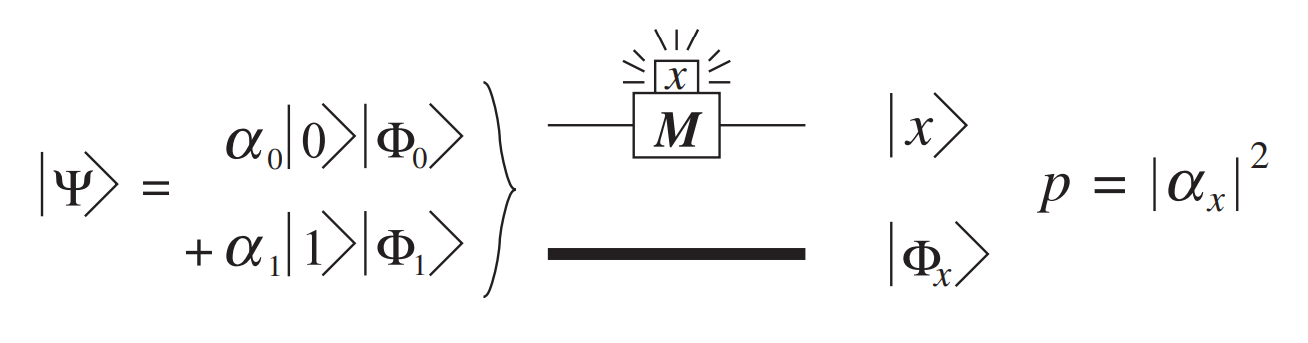
\includegraphics[scale=0.25]{measurement}
\end{figure}

The stronger form of the Born rule applies when one measures only a single one of $n+1$ Qbits by sending it through a standard 1-Qbit measurement gate. The general form of the $(n+1)$ Qbits is given by
\begin{align}
\ket{\Psi}_{n+1} = \sum^{2^{n+1}-1}_{x=0}\gamma(x)\ket{x}_{n+1}, \quad \sum^{2^{n+1}-1}_{x=0}\abs{\gamma(x)}^2 = 1
\end{align}
from which we write explicitly as a combination of the measured Qbit and the other $n$ Qbits:
\begin{align}
\ket{\Psi} = \alpha_0\ket{0}\ket{\Phi_0}_n + \alpha_1 \ket{1}\ket{\Phi_1}_n
\end{align}
where
\begin{align}
\ket{\Phi_0}_n = \f{1}{\alpha_0}\sum^{2^{n}-1}_{x=0}\gamma(x)\ket{x}_n; \quad 
\ket{\Phi_1}_n = \f{1}{\alpha_1}\sum^{2^{n}-1}_{x=0}\gamma(2^n+x)\ket{x}_n
\end{align}
and of course to normalize things
\begin{align}
\alpha^2_0 = \sum^{2^n-1}_{x=0}\abs{\gamma(x)}^2, \quad \alpha^2_1 = \sum^{2^n-1}_{x=0}\abs{\gamma(2^n + x)}^2.
\end{align}
Note that $\ket{\Phi_0}_n$ and $\ket{\Phi_1}_n$ are not necessarily orthogonal.\\

In plain English, the rule asserts that if one measures only the single Qbit whose state symbol is explicitly separated out from the other $n$ Qbits, then the measurement gate will produce $x$ (0 or 1) with probability $\abs{\alpha_x}^2$. The resulting state vector will be the product state $\ket{x}\ket{\Phi_x}_n$. \\

If the Qbit being measured is initially unentangled with the other $n$ Qbits, then the action of the measurement gate on the measured Qbit is just that specified by the Born rule. The unmeasured Qbits are as if they are not there and remain in their original states throughout the process. 

\begin{figure}[!htb]
	\centering
	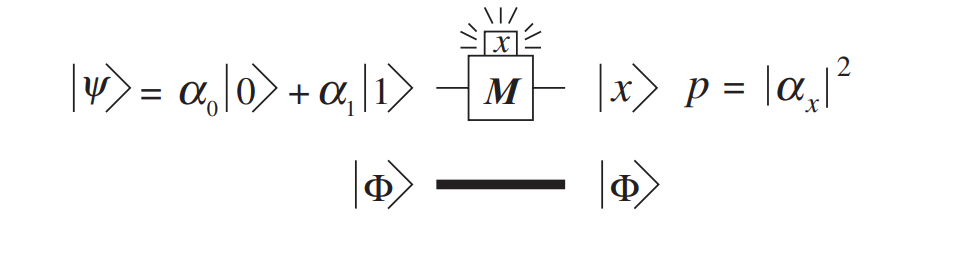
\includegraphics[scale=0.25]{measurement1}
\end{figure}

Applying the generalized Born rule $n$ times to successive 1-Qbit measurements of each of $n$ Qbits initially in $\ket{\psi}_n$, one can show that the final state is $x$ with probability $\abs{\alpha_x}^2$.  Hence, there is only a single primitive piece of measurement hardware: the 1-
Qbit measurement gate. \\

Even more generally, suppose we have the general state of $m+n$ Qbits:
\begin{align}
\ket{\psi}_{m+n} = \sum^{2^m}_{x=0}\alpha_x\ket{x}_m\ket{\Phi_x}_n
\end{align}
where $\sum_x\abs{\alpha_x}^2 = 1$ and the states $\ket{\Phi_x}$ are normalized but not necessarily orthogonal. Applying the Born rule $m$ times to $m$ Qbits we see that if just $m$ Qbits ($\ket{x}_m$) are measured, then with probability $\abs{\alpha_x}^2$ the result will be $x$, and the resulting state vector will be the product state $\ket{x}_m\ket{\Phi_x}_n$.


\subsection{Measurement gates and state preparation}

The measurement gate is useful for producing states with definite states. A measurement that registers $x$ outputs a state in the classical basis $\ket{x}_n$. If we then $\X$ each Qbit that registered a 1 in the measurement and do nothing to the Qbits that registered a 0 then the resulting Qbits will be in the state $\ket{0}_n$. Most quantum-computational algorithms take this state as its input. \\

Measurement gates therefore plays two role: \textit{state preparation} and extracting information from the Qbits. 


\subsection{Constructing arbitrary 1- and 2-Qbit states}

We will first consider the case for a single Qbit. Let $\ket{\psi}$ be any 1-Qbit state, and let $\ket{\phi}$ be an orthogonal state, i.e. $\braket{\psi}{\phi} = 0$. The state $\ket{\phi}$ is unique up to an overall phase. Because $\ket{0}$ and $\ket{1}$ are linearly independent, there is a unique linear transformatin taking them into $\ket{\psi}$ and $\ket{\phi}$. Also, because $\ket{\phi}$ and $\ket{\psi}$ are orthonormal, this linear transformation must be unitary. We will call it $\mathbf{u}$, where
\begin{align}
\ket{\psi} = \mathbf{u}\ket{0}.  
\end{align}
By showing the existence of such a unitary gate $\mathbf{u}$, we're done. \\

Any arbitrary unentangled 2-Qbit state, which is just a fancy way to say it is a tensor product of two 1-Qbit states, can be constructed out of $\ket{00}$ by applying a tensor product of two unitaries to each of the $\ket{0}$ individual states. This follows from the previous argument. To sum this up, we say that an unentangled state requires an unentangled gate to prepare. \\

When the 2-Qbit state is entangled, however, its production requires a 2-Qbit gate that is not a tensor product of two single-Qbit unitaries. The solution, as it turns out, is using a combination of a single cNOT gate and some 1-Qbit unitaries. Consider the general 2-Qbit state:
\begin{align}
\ket{\Psi} = \alpha_{00}\ket{00} + \alpha_{01}\ket{01} + \alpha_{10}\ket{10} + \alpha_{11}\ket{11}.
\end{align}
Observe that this can be re-written in the following way:
\begin{align}
\ket{\Psi} = \ket{0}\otimes \ket{\psi} + \ket{1}\otimes\ket{\phi}
\end{align}
where $\ket{\phi} = \alpha_{00}\ket{0} + \alpha_{01}\ket{1}$ and $\ket{\phi} = \alpha_{10}\ket{0} + \alpha_{11}\ket{1}$.  \\

Next, consider a unitary $\mathbf{u}$ whose action on the computational basis is the following:
\begin{align}
\mathbf{u}\ket{0} = a\ket{0} + b\ket{1}, \quad \mathbf{u}\ket{1} = -b^*\ket{0} + a^*\ket{1}
\end{align}
where $\abs{a}^2 + \abs{b}^2=  1$, as usual. Applying $\mathbf{u}\otimes \Id$ to $\ket{\Psi}$, we get
\begin{align}
\lp\mathbf{u}\otimes \Id\rp \ket{\Psi} &= \lp a\ket{0} + b\ket{1}  \rp\otimes\ket{\psi} +  \lp -b^*\ket{0} + a^*\ket{1}\rp\otimes\ket{\phi}\nn\\
&= \ket{0}\otimes \ket{\psi'} + \ket{1}\otimes \ket{\phi'}
\end{align}
where
\begin{align}
\ket{\psi'}= a\ket{\psi} - b^*\ket{\phi}; \quad \ket{\phi'} = b\ket{\psi} + a^*\ket{\phi}.
\end{align}
Now, if $\ket{\psi'}$ and $\ket{\phi'}$ are orthogonal, then we're done. We wish to choose complex numbers $a,b$ to achieve this. Consider the inner product of $\ket{\psi'}$ and $\ket{\phi'}$:
\begin{align}
\braket{\phi'}{\psi'} = a^2\braket{\phi}{\psi} - b^2\braket{\phi}{\phi} + {ab^*\lp \braket{\psi}{\psi} - \braket{\phi}{\phi} \rp}
\end{align}
If $\braket{\psi}{\phi} \neq 0$ then setting $\braket{\phi'}{\psi'}$ to 0 gives an quadratic equation for the ratio $a/b^*$ = 0, for which there are two complex solutions. Setting $a$ determines a $\mathbf{u}$ for which
\begin{align}
\lp \mathbf{u}\otimes \Id \rp\ket{\Psi} = \ket{0}\otimes\ket{\psi'} + \ket{1}\otimes\ket{\phi'}
\end{align} 
where $\braket{\psi'}{\phi'} = 0$. If $\braket{\phi}{\psi} =0$ then there's nothing else for us to do. $\mathbf{u} \equiv \Id$. \\

Let $\lambda, \mu$ be positive reals such that 
\begin{align}
\ket{\psi''} = \f{\ket{\psi'}}{\lambda}, \quad \ket{\phi''} = \f{\ket{\phi'}}{\mu}
\end{align}
are normalized. This makes $\ket{\psi''}$ and $\ket{\phi''}$ an orthonormal pair. Following an argument earlier, there exists a unitary $\mathbf{v}$ for which 
\begin{align}
\ket{\psi''} = \mathbf{v}\ket{0}, \quad \ket{\phi''} = \mathbf{v}\ket{1}.
\end{align} 
From here, we see that 
\begin{align}
\ket{\Psi} = \lp \mathbf{u}^\dagger \otimes \mathbf{v} \rp\lp \lambda\ket{0}\otimes \ket{0} + \mu\ket{1}\otimes \ket{1} \rp.
\end{align}
Now, note that $\mathbf{C}_{10}\ket{00} \to \ket{00}$ and $\mathbf{C}_{10}\ket{10} \to \ket{11}$. So we can write the equality as follows
\begin{align}
\ket{\Psi} = \lp \mathbf{u}^\dagger \otimes \mathbf{v} \rp \mathbf{C}_{10} \lp \lambda\ket{0} + \mu\ket{1}\rp\otimes \ket{0}.
\end{align}
But we're not finished. Remember that we wish to obtain $\ket{\Psi}$ from $\ket{00} = \ket{0}\otimes \ket{0}$. However, we're very close now, as we only need to obtain $\lambda\ket{0} + \mu\ket{1}$ from $\ket{0}$. Fortunately, we already know how to do this! Consider another unitary $\mathbf{w}$ for which 
\begin{align}
\mathbf{w}\ket{0} = \lambda\ket{0} + \mu\ket{1}
\end{align}
whose existence is guaranteed by our earlier arguments. So, with a single cNOT and three unitaries, we can prepare any entangled 2-Qbit state from $\ket{00}$ via
\begin{align}
\ket{\Psi} = \lp \mathbf{u}^\dagger \otimes \mathbf{v} \rp \mathbf{C}_{10}\lp\mathbf{w}\otimes \Id\rp\ket{00}.
\end{align}












\newpage



\section{Examples}


\subsection{The general computational process}
In general, we need at least $n+m$ Qbits for computations, where $n$ is the number of Qbits required to specify the input $x$, and $m$ is the number of Qbits required to specify the output $f(x)$. The set of $n$ Qbits is called the \textit{input register}. The set of $m$ Qbits is called the \textit{output register}. Havig separate input and output registers is standard practice in the classical theory of reversible computation. Since quantum computers must operate reversibly, they are generally designed to operate with both input and output registers. \\

We view a quantum computation $f$on $n+m$ Qbits as a unitary transformation $\mathbf{U}_f$ acting on the $n+m$ Qbit states:
\begin{align}
\mathbf{U}_f (\ket{x}_n\ket{y}_m) = \ket{x}_n \ket{y\oplus f(x)}_m
\end{align}
where $\oplus$ indicates mod 2 addition, or XOR. If $y=0$  then 
\begin{align}
\mathbf{U}_f(\ket{x}_n \ket{0}_m) = \ket{x}_n \ket{f(x)}_m
\end{align}
so we have $f(x)$ in the output register, while the input register $\ket{x}_n$ is intact (and is independent on the state of $y$). \\

Clearly, $\mathbf{U}_f$ is its own inverse:
\begin{align}
\mathbf{U}_f\mathbf{U}_f (\ket{x}\ket{y}) = \mathbf{U}_f(\ket{x}\ket{y\oplus f(x)}) = \ket{x}\ket{y\oplus f(x)\oplus f(x)} =\ket{x}\ket{y}.
\end{align} 
Now, if we apply to each Qbit in the 2-Qbit state $\ket{0}\ket{0}$ the 1-Qbit Hadamard, then we get
\begin{align}
(\had \otimes \had)(\ket{0}\otimes \ket{0}) &= (\had\ket{0})\otimes(\had\ket{0})\nn\\
&= \f{1}{\sqrt{2}}(\ket{0} + \ket{1}) \otimes \f{1}{\sqrt{2}}(\ket{0} + \ket{1})\nn\\
&= \f{1}{2}(\ket{00} + \ket{01} + \ket{10} + \ket{11})\nn\\
&= \f{1}{2}(\ket{0}_2 + \ket{1}_2 + \ket{2}_2 + \ket{3}_2).
\end{align}
This generalizes to the $n$-fold tensor product of $n$ Hadamards, applied to the $n$-Qbit state $\ket{0}_n$:
\begin{align}
{\had^{\otimes n}\ket{0}_n = \f{1}{2^{n/2}}\sum_{0 \leq x \leq 2^n} \ket{x}_n}
\end{align}

If the initial state of the input register is $\ket{0}_n$, then the output state is the perfect superposition of all possible $n$-Qbit inputs. If we than apply $\mathbf{U}_f$ to that superposition, with $0$ initially in the output register, then we get
\begin{align}
\mathbf{U}_f (\had^{\otimes n} \otimes \Id_m)(\ket{0}_n\ket{0}_m) &= \f{1}{2^{n/2}}\sum_{0\leq x\leq 2^n} \mathbf{U}_f (\ket{x}_n \ket{0}_m)\nn\\
&= \f{1}{2^{n/2}} \sum_{0\leq x\leq 2^n} \ket{x}_n \ket{f(x)}_m.
\end{align}

Why is this important? This is called \textit{quantum parallelism}. If before letting $\mathbf{U}_f$ act, we only apply the $\had$ transformation to every Qbit of the input register (all initially in 0), then the result of the computation s described by a state whose structure cannot be explicitly specified without knowing the result of all $2^n$ evaluations of the function $f$. So, if we start with 100 Qbits in the input register, if a hundred Hadamard gates act on the input register before the application of $\mathbf{U}_f$, then the form of the final state contains the results of $2^{100} \approx 10^{30}$ evaluations of the function $f$! \\

Another ``miracle'' is that we can't say the result of the computation is \textit{actually} $2^n$ evaluations of $f$, because when we have a collection of Qbits in a definite but unknown state, there is no way to find out what that state is.



\subsection{No-cloning theorem}

If there were a way to make copies of the output state prior to making measurements (without running the whole computation again) then one could learn the values of $f$ for several different values of $x$. However, this is forbidden by the so-called \textit{no-cloning theorem}. \\


The no-cloning theorem is a consequence of linearity. Suppose to get a contradiction that cloning is possible, i.e. 
\begin{align}
\mathbf{U}(\ket{\psi}\ket{0}) = \ket{\psi}\ket{\psi}, \quad \mathbf{U}(\ket{\phi}\ket{0}) = \ket{\phi}\ket{\phi}
\end{align}
then from linearity:
\begin{align}
\mathbf{U}(a\ket{\psi} + b\ket{\phi})\ket{0} = a\ket{\psi}\ket{\psi} + b\ket{\phi}\ket{\phi}.
\end{align}
But if $\mathbf{U}$ closed arbitrary inputs, we would also have
\begin{align}
\mathbf{U}(a\ket{\psi} + b\ket{\phi})\ket{0} &= (a\ket{\psi} + b\ket{\phi})(a\ket{\psi} + b\ket{\phi})\nn\\
&= a^2\ket{\psi}\ket{\psi} + b^2\ket{\phi}\ket{\phi} + ab\ket{\phi}\ket{\phi} + ab\ket{\phi}\ket{\psi}\nn\\
&\neq a\ket{\psi}\ket{\psi} + b\ket{\phi}\ket{\phi}
\end{align}
unless $ab=0$. \\

Okay, but what about creating a reasonable, but not quite exact, clone? Suppose
\begin{align}
\mathbf{U}(\ket{\psi}\ket{0}) \approx \ket{\psi}\ket{\psi}, \quad \mathbf{U}(\ket{\phi}\ket{0}) \approx \ket{\phi}\ket{\phi}
\end{align}
then since $\mathbf{U}$ preserves the inner product we must have that
\begin{align}
\braket{\phi}{\psi} \approx \braket{\phi}{\psi}^2.
\end{align}
But this means that $\braket{\phi}{\psi}$ is close to either 0 or 1. This means that $\mathbf{U}$ does well only if $\ket{\psi}$ and $\ket{\phi}$ are very nearly the same, or are very nearly orthogonal. In any case, $\mathbf{U}$ isn't too useful. 








\subsection{Deutsch's problem}




The Deutsch's problem is an example of a quantum tradeoff that sacrifices particular information to acquire relational information.\\

Consider only functions $f$ that take a single bit into a single bit. There are only 4 such functions, since there are two possibilities for the input and two possibilities for the output. These functions are
\begin{align}
&\mathbf{U}_{f_0} \equiv \Id\\
&\mathbf{U}_{f_1} \equiv \mathbf{C}_{io}\\
&\mathbf{U}_{f_2} \equiv \mathbf{C}_{io}\X_o\\
&\mathbf{U}_{f_3} \equiv \X_o
\end{align}
where of course $i,o$ are for \textit{input} and \textit{output}, respectively. In general,
\begin{align}
\mathbf{U}_f(\ket{x}\ket{y}) = \ket{x}\ket{y\oplus f(x)}.
\end{align}
Schematically, this looks like
\begin{figure}[!htb]
	\centering
	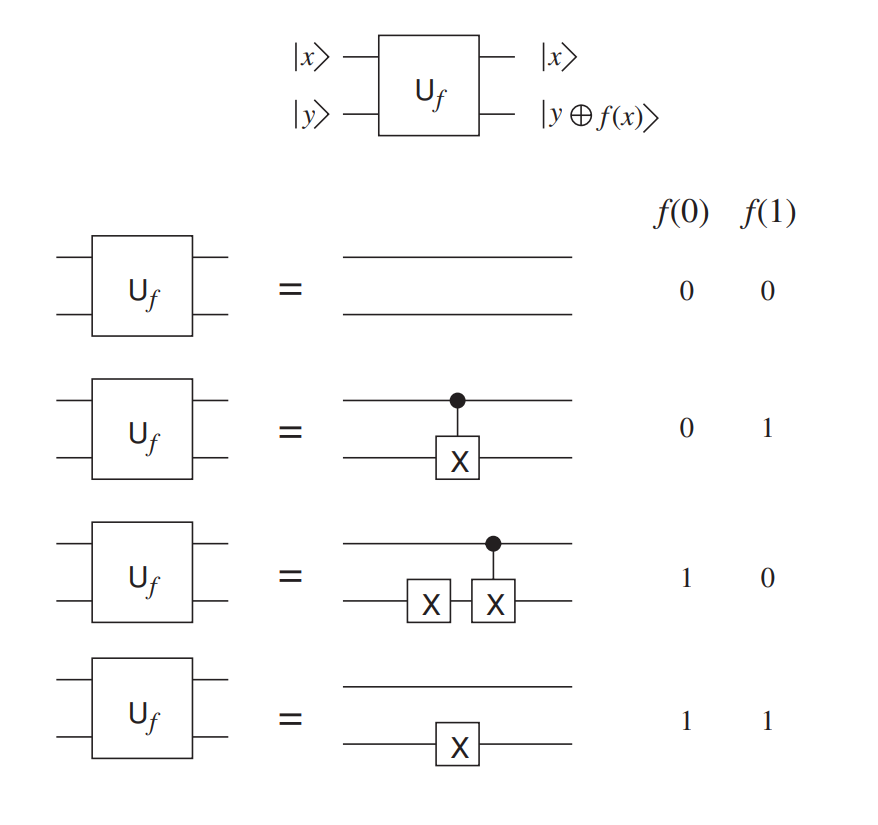
\includegraphics[scale=0.5]{U}
	\caption{By Mermin}
\end{figure}
When $f$ is unknown, we can find out what $f$ is by letting $\mathbf{U}_f$ act twice, once on $\ket{0}\ket{0}$ and then on $\ket{1}\ket{0}$. But what if we could only let it act once? And what if we are only interested in knowing whether $f$ is constant (in which case it is $f_1$ or $f_3$) or not constant ($f_2$ or $f_4$)? With a classical computer, we will have to evaluate both $f(1)$ and $f(0)$, but with a quantum computer we only need to let $\mathbf{U}_f$ act once, only with the tradeoff of not knowing the values of $f(0)$ and $f(1)$.  \\

To do this we use the Hadamard to put the input into superposition:
\begin{align}
\mathbf{U}_f (\had \otimes \Id) (\ket{0}\ket{0}) = \f{1}{\sqrt{2}}\ket{0}\ket{f(0)} + \f{1}{\sqrt{2}}\ket{1}\ket{f(1)}.
\end{align}
This doesn't solve the problem, but we see that we can make further unitary transformations to the state above before making measurements that enable us half the time to state with assurance whether or not $f(0) = f(1)$. \\

Suppose that instead of starting with letting the Hadamard act on the input of $\ket{0}\ket{0}$, we let two Hadamards act on $\ket{1}\ket{1}$, i.e. 
\begin{align}
(\had\otimes \had)(\X \otimes \X)(\ket{0}\ket{0}) &= (\had \otimes \had)(\ket{1}\otimes \ket{1})\nn\\
&= \lp\f{1}{\sqrt{2}}\ket{0} - \f{1}{\sqrt{2}}\ket{1} \rp \lp\f{1}{\sqrt{2}}\ket{0} - \f{1}{\sqrt{2}}\ket{1} \rp \nn\\
&= \f{1}{2}\lp \ket{0}\ket{0} - \ket{1}\ket{0} - \f{0}{1} + \ket{1}\ket{1} \rp.
\end{align}
Then, letting $\mathbf{U}_f$ act on this state to get
\begin{align}
\mathbf{U}_f (\had\otimes \had)(\X \otimes \X)(\ket{0}\ket{0}) &= \dots\nn\\
&= \f{1}{2}\lp \ket{0}\ket{f(0)} - \ket{1}\ket{f(1)} - \ket{0}\ket{1 \oplus {f}(0)} + \ket{1}\ket{1\oplus {f}(1)} \rp\nn\\
&\equiv \f{1}{2}\lp \ket{0}\ket{f(0)} - \ket{1}\ket{f(1)} - \ket{0}\ket{\tilde{f}(0)} + \ket{1}\ket{\tilde{f}(1)} \rp
\end{align}
where we have defined
\begin{align}
\tilde{f} \equiv 1 \oplus f.
\end{align}
Now, if $f(0) = f(1)$ then the state above becomes
\begin{align}
\f{1}{2}\lp \ket{0} - \ket{1} \rp \lp \ket{f(0)} - \ket{\tilde{f}(0)} \rp, \quad f(0) = f(1)
\end{align}
else ($f(0) \neq f(1)$) then the state above becomes
\begin{align}
\f{1}{2}\lp \ket{0} + \ket{1} \rp \lp \ket{f(0)} - \ket{\tilde{f}(0)} \rp, \quad f(0) \neq f(1)
\end{align}
since $f(1) = \tilde{f}(0)$ whenever $f(0) \neq f(1)$.\\

Now, because
\begin{align}
\had \lp \ket{0} \pm \ket{1} \rp  &= \f{1}{\sqrt{2}}\lp \ket{0} + \ket{1} \rp \pm \f{1}{\sqrt{2}}\lp \ket{0} - \ket{1} \rp\nn\\
&= \begin{cases}
\sqrt{2}\ket{0}, \quad (+) \\ 
\sqrt{2}\ket{1}, \quad (-)
\end{cases},
\end{align}
when we let $\had$ act on the \textit{input} register of the state above, we have
\begin{align}
\begin{cases}
\ket{1}\f{1}{\sqrt{2}}\lp \ket{f(0)} - \ket{\tilde{f}(0)} \rp, \quad f(0) = f(1)\\
\ket{0}\f{1}{\sqrt{2}}\lp \ket{f(0)} - \ket{\tilde{f}(0)} \rp, \quad f(0) \neq f(1)
\end{cases}.
\end{align}
Putting everything together we have
\begin{align}
\boxed{(\had \otimes \Id) \mathbf{U}_f (\had \otimes \had) (\X \otimes \X)(\ket{0}\ket{0}) = \begin{cases}
\ket{1}\f{1}{\sqrt{2}}\lp \ket{f(0)} - \ket{\tilde{f}(0)} \rp, \quad f(0) = f(1)\\
\ket{0}\f{1}{\sqrt{2}}\lp \ket{f(0)} - \ket{\tilde{f}(0)} \rp, \quad f(0) \neq f(1)
\end{cases}}
\end{align}
Now, notice that the state of the input register will be $\ket{1}$ if $f(0) = f(1)$, and $\ket{0}$ if $f(0) \neq f(1)$. So, by measuring the input register, we can tell if $f$ is constant. \\

Notice that the output register in both cases are the same (differ only in the sign, but that doesn't make the state distinguishable). But in any case, we learn whether or not $f$ is constant by calling $\mathbf{U}_f$ only once. 









\subsection{Why additional Qbits needn't mess things up}

\begin{figure}[!htb]
	\centering
	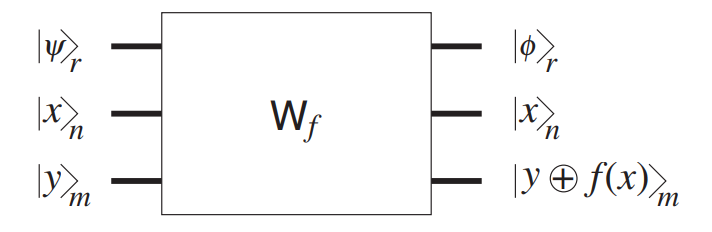
\includegraphics[scale=0.5]{mnr}
\end{figure}


We use $n+m$ Qbits to perform quantum computations, where $n$ is the number of Qbits in the input register and $m$ in the output register. In general, however, we also need $r$ additional Qbits. The action of the computer on these Qbits is then described by a unitary $\mathbf{W}_f$, which acts on all $m+n+r$ Qbits. Only in special cases do we have $\mathbf{W}_f$ act separately on the input and output registers and leaving the additional Qbits alone. In general, the $r$ additional Qbits get entangled with the $m+n$ Qbits too. \\

Let the initial state be
\begin{align}
\ket{\Psi}_{n+m+r} = \ket{x}_n \ket{y}_m \ket{\psi}_r
\end{align}
then applying the global unitary gate $\mathbf{W}_f$ gives:
\begin{align}
\mathbf{W}_f \ket{\Psi}_{n+m+r} = \ket{x}_n \ket{y+\oplus f(x)}_m \ket{\phi}_r.
\end{align}
The state of the addition Qbits is not necessarily intact. However, we require that the additional Qbits are not only unentangled with the input and output registers, but also its state $\ket{\phi}_r$ is independent of the initial state of the input and output registers. When this is the case, the action of $\mathbb{W}_f$ on $n+m$ Qbits can be represented by the unitary $\mathbf{U}_f$ on the subspace $n+m$ alone, while the $r$ additional Qbits are taken from the initial pure state $\ket{\psi}_r$ to a final pure state $\ket{\phi}_r$ that is independent of the initial contents of the input and output registers. \\

So how do we construct $\mathbf{W}_f$ so that it acts as if $\mathbf{U}_f$ is acting on the $n+m$ Qbits alone and leaving the additional Qbits intact? Schematically, this looks like
\begin{figure}[!htb]
	\centering
	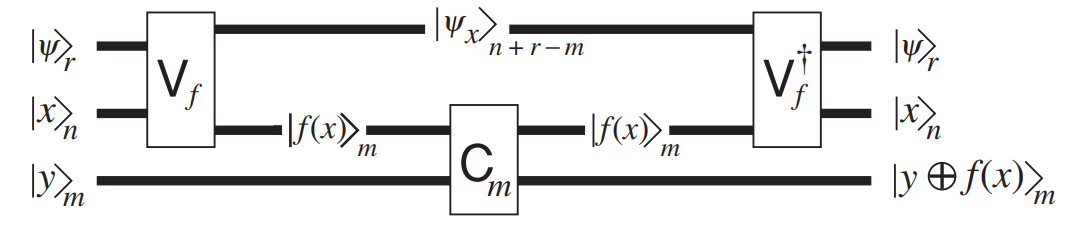
\includegraphics[scale=0.6]{W}
\end{figure} 

There are three steps to the solution:
\begin{enumerate}
	\item First, we apply a unitary transformation $\mathbf{V}$ that acts only on the $n$ and $r$ input register and additional Qbits. We can design the $\mathbf{V}$ gate such that if the initial input state is $\ket{x}_n$ and $\ket{\psi}_r$ then the output is $\ket{f(x)}_m$ and $\ket{\psi}_{n+r-m}$. We will then proceed to feed $\ket{f(x)}_m$ to the next gate.
	\item In this step, we let $y$ change into $y\oplus f(x)$ without changing the states of the other $n+r$ Qbits. This can be done with $m$ CNOT gates that combine to make a single unitary $\mathbf{C}_m$ gate. The control bits here will be the bits in $\ket{f(x)}_m$, so they remain unchanged. Only the $\ket{y}_m$ Qbits states get changed. 
	\item Finally, because the state of the $n+r$ Qbits is not altered by $\mathbf{C}_m$, we simply let $\mathbf{V}^\dagger$ reverse these back to their original states, to give us the original $\ket{\psi}_r$, $\ket{x}_n$, with $\ket{y\oplus f(x)}_m$ 
\end{enumerate}


As an aside, the $m$ CNOT gate, for $m=5$, looks like
\begin{figure}[!htb]
	\centering
	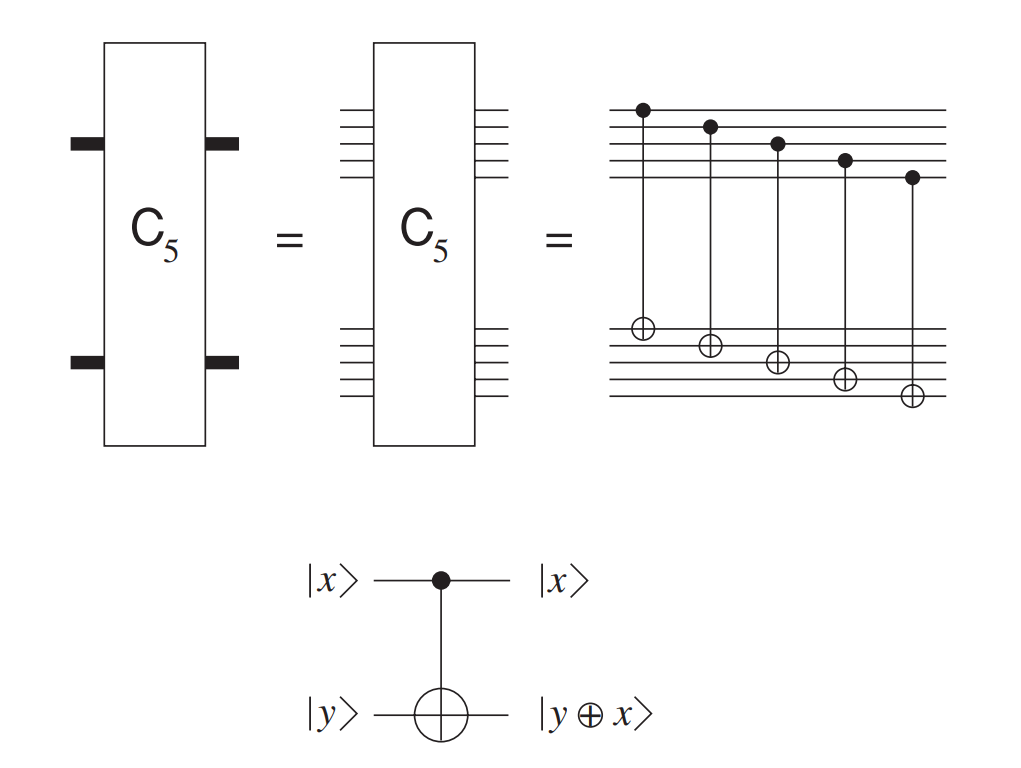
\includegraphics[scale=0.6]{mcnot}
\end{figure}





























\subsection{The Bernstein-Vazirani problem}

Consider the function $f(x) = a \cdot x$, where $a\cdot x$ denotes the the mod-2 sum of the products of the corresponding bits of $a$ and $x$, i.e., 
\begin{align}
a\cdot x = \bigoplus_{i=0} a_0 x_0
\end{align}
where of course $a_i, x_i$ take values $\{ 0,1\}$, and $a$ is a non-negative integer less than $2^n$. The problem is to find $a$. More specifically, suppose we have a subroutine which evaluates $f(x) = a\cdot x$, how many times do we have to query $f(x)$ in order to find what $a$ is? Note that the a rule one has to follow here is that any additional Qbits used by the algorithm (so, except for the input and output registers) must return to their initial state once the evaluation has completed. Notice that the answer we get is either a 0 or 1, so we need only one Qbit in the output register for this.  \\

Classically, here's how we do it. Let a number $a$ be given. Because the expansion of $2^m$ has a 1 in position $m$ and 0 in all other positions, the $m^{\text{th}}$ bit of $a$ is $a\cdot 2^m$ (it's easy to see how this works by writing down the mod-2 inner product).  This means that with a classical computer, we can learn the values of $n$ bits of $a$ by applying $f$ to $x = 2^m$, $m \in [0,n]$, $n$ times.  This requires querying $f$ $n$ times. \\

Quantum computers, on the other hand, requires a \textbf{single} query to completely determine $a$, regardless of how big $n$ is. There are two ways to discuss how this works. The first way goes into the algebra, while the second gives pictorial, circuit-theoretical approach to solving this problem. I won't worry about the second approach and will only focus on the first approach. \\

The (conventional) first way to do this exploits a trick that is useful in dealing with functions like $f$ that act on $n$ Qbits without output to a single Qbit. Suppose the 1-Qbit output register is initially prepared in the state $\had \X \ket{0} = \had\ket{1} = (1/\sqrt{2})(\ket{0} - \ket{1})$. We know that 
\begin{align}
\U_f \ket{x}_n\ket{y}_1 = \ket{x}_n\ket{y\oplus f(x)}  = \ket{x}_n\ket{\bar{y}}_1 \iff f(x) = 1.
\end{align} 
This means
\begin{align}
\U_f \ket{x}_n\f{1}{\sqrt{2}}\lp \ket{0} - \ket{1} \rp = (-1)^{f(x)}\ket{x}_n \f{1}{\sqrt{2}}\lp \ket{0} - \ket{1} \rp.
\end{align}
We see that by taking the state of the 1-Qbit output register to be $(1/\sqrt{2})(\ket{0} - \ket{1})$, we convert a bit flip to an overall change of sign. This is the first trick. The second trick is not exactly a trick, but a fact that we will see in the homework:
\begin{align*}
\had^{\otimes n}\ket{x}_n = \f{1}{\sqrt{2^n}} \sum_{0\leq y < 2^n}(-1)^{x\cdot y}\ket{y}.
\end{align*}
With this, if we start with the $n$-Qbit input register in the standard initial state $\had^{\otimes n}\ket{0}$, put the 1-Qbit output register into $\had\ket{1}$, apply $\U_f$, and then again apply $\had^{\otimes n}$ to the input register we will get
\begin{align}
(\had^{\otimes n} \otimes \Id)\U_f(\had^{\otimes n} \otimes \had)\ket{0}_n\ket{1}_1 = \f{1}{2^n}\sum_{0\leq x,y< 2^n}(-1)^{f(x)+x\cdot y}\ket{y}\f{1}{\sqrt{2}}\lp \ket{0} - \ket{1} \rp.
\end{align}
I will spare the reader the details of this calculation. Parts of this calculation will be verified in the exercises. By inspection, however, the reader should be able to convince himself this result makes sense. \\

From here, we do sum over $x$ first. If $f(x) = a\cdot x$ then the sum over $x$ produces the factor
\begin{align}
\sum_{0\leq x < 2^n}(-1)^{a\cdot x +  x\cdot y} = \prod_{j=1}^n \sum_{x_j\in \{0,1\}} (-1)^{(a_j + y_j)x_j}.
\end{align}
At least one term in the product is zero unless every bit $y_j$ of $y$ is equal to the corresponding bit $a_j$ of $a$, i.e., unless $y=a$ (check this by inspection). Therefore, if I apply a final $\had$ onto the 1-Qbit output register to make things a little nicer, then the entire computational process reduces to
\begin{align}
\had^{\otimes (n+1)}\U_f \had^{\otimes (n+1)}\ket{0}_n\ket{1}_1 = \ket{a}_n\ket{1}_1.
\end{align} 
So by putting the input and output registers into the appropriate initial states, after a single call for the subroutine followed by $\had^{\otimes n}$ to the input register, the state of the input register becomes $\ket{a}$. Now, all $n$ bits of the number $a$ can ne determined by measuring the input register, even though we have called the subroutine only once.













   














\subsection{Simon's problem}


In the Bernstein-Vazirani problem, a classical computer must call the subroutine $n$ times, while a quantum computer only need to call the subroutine once. As the problem grows, the classical complexity scales linearity, while the quantum complexity is still constantly one. In the Simon's problem, the speed-up is even more dramatic. The classical complexity grows exponentially with the size of the problem, while the quantum complexity only grows linearly. \\

This speed-up involves a probabilistic element characteristic of many quantum computations. The characterization of how the number of calls of the subroutine scales with the number of bits in $a$ applies not to calculating directly, but to learning it with probability very close to 1. \\

The subroutine $\U_f$ in Simon's problem evaluates a function $f$ on $n$ bits is two to one, i.e., it is a function from $n$ to $n-1$ bits. It is constructed so that the $n$-bit integers $x$ and $y$ are related by $x = y\oplus a \iff x \oplus y = a$. This is essentially a period-finding problem:
\begin{align}
f(x \oplus a) =  f(x).
\end{align} 
Of course the period here is $a$. Simon's problem is a precursor of Shor's period-finding algorithm where one finds the period $a$ under the ordinary addition $f(a+x) = f(x)$. \\

With a classical computer, what you have to do to find $a$ is feeding the subroutine with a bunch of $x$, and compare $f(x\oplus a)$ against $f(x)$ until you see a match. At any stage of the process prior to success, if you have picked $m$ different values of $x$, then all you know is that $a\neq x_i \oplus x_j$ for all pairs $x_i,x_j$. This means you have eliminated at most $(m/2)(m-1)$ values of $a$. Now, there are $2^n-1$ possible values for $a$. The chance of success won't be large unless  $(m/2)(m-1)$ is sufficiently close to $2^n$. This means $m\sim 2^{n/2}$ is required. This means the number of trials grows exponentially. \\

In (spectacular) contrast, a quantum computer can determine $a$ with not much more than $n$ queries. Let's see how this is done:\\

To do this we first return to the standard procedure and let $\U_f$ act on $\had^{\otimes n}\ket{0}_n$. This gives
\begin{align}
\U_f (\had^{\otimes} \ket{0}_n) = \f{1}{2^{n/2}}\sum_{0\leq x < 2^n} \ket{x}\ket{f(x)}
\end{align}
which the reader can verify from the results in the exercises. \\

Now, if we subject only the output register to a measurement, then the measurement gate is equally likely to indicate each of the $2^{n-1}$ different values of $f$. Looking at the RHS of the equation above again, since $f$ is periodic, we know that each value of $f$ appears in two terms that have the same amplitudes. The Born rule (of partial measurement) tells us that the input register must be in the state
\begin{align}
\f{1}{\sqrt{2}}\lp \ket{x_0} + \ket{x_0 \oplus a} \rp
\end{align}
for that value $x_0$ for which $f(x_0)$ agrees with the random value of $f$ given by the measurement. \\

This looks good, because we just created a superposition of just two computational basis states, associated with two $n$-bit integers, that differ in $\oplus$ by $a$. If we knew these two integers their bitwise mod 2 sum would be $a$. However, when a register is in quantum state there is no way to learn what state it is in. By subjecting the state above to a direct measurement all we can learn is either $x_0$, a random number, or $x_0 \oplus a$, another random number. $a$ appears only in the relation between these two integers, only one of which we know.\\

But we can cure this problem. Just like in the Deutsch's problem, we can ignore the possibility of learning either number. It is possible that by applying some operations before measuring can let us extract the relation $a$. This operation is $\had^{\otimes n}$:
\begin{align}
\had^{\otimes n}\f{1}{\sqrt{2}}\lp \ket{x_0} + \ket{x_0 \oplus a} \rp &= \f{1}{\sqrt{2^{n+1}}}\sum_{0\leq y < 2^n} \lp (-1)^{x_0\cdot y} + (-1)^{(x_0\oplus a)\cdot y} \rp \ket{y}\nn\\
&= \f{1}{\sqrt{2^{n-1}}} \sum_{a\cdot y = 0}(-1)^{x_0\cdot y}\ket{y}.
\end{align}  
If we now measure the input register, we learn with equal probability any of the values of $y$ for which $a\cdot y = 0$. With this, each call for $\U_f$ gives us a $y$ such that $a\cdot y =0$. \\

Next, we want to show that this enables us to determine $a$ with high probability with not many more than $n$ calls for $\U_f$. With a single call for $\U_f$, unless we get $y=0$ (which is unlikely), we learn a nonzero value of $y$, and therefore a nontrivial subset of the $n$ bits of $a$ whose mod 2 sum vanishes. This means we have cut the number of possible choice for $a$ by a half, from $2^n-1$ to $2^{n-1}-1$. If we repeat this procedure, we will likely learn another nonzero value of $y$ that isn't a repeat of the previous $y$. This enables us to again halve the number of possible candidates for $a$. It turns out (after from mathematical analysis) that with $n+x$ calls for $\U_f$ the probability $q$ of acquiring enough information to determine $a$ is
\begin{align}
q = \lp 1-\f{1}{2^{x+n}}\rp \lp 1-\f{1}{2^{x+n-1}}\rp \dots \lp 1-\f{1}{2^{x+2}} \rp \geq 1-\f{1}{2^{x+1}}.
\end{align} 










%\subsection{Constructing Toffoli gates}



\newpage


\section{The Quantum Fourier Transform \& Applications}


\subsection{The QFT}
\subsection{Phase estimation}
\subsubsection{Performance and requirements}
\subsection{Applications: order-finding and factoring}
\subsubsection{Order-finding}
\subsubsection{Factoring}
\subsection{General applications of the QFT}
\subsubsection{Period-finding}
\subsubsection{Discrete algorithms}
\subsubsection{The hidden subgroup problem}
\subsubsection{Other quantum algorithm?}

\newpage



\section{Quantum search algorithm}

\subsection{The quantum search algorithm}
\subsubsection{The oracle}
\subsubsection{The procedure}
\subsubsection{Geometric visualization}
\subsubsection{Performance}
\subsection{Quantum search as a quantum simulation}
\subsection{Quantum counting}
\subsection{Speeding up the solution of $\mathbf{NP}$-complete problems}
\subsection{Quantum search of an unstructured database}
\subsection{Optimality of the search algorithm}
\subsection{Black box algorithm limits}





\newpage


\section{Breaking NSA encryption}

\subsection{Preiod finding, factoring, and cryptography}
\subsection{Number-theoretic preliminaries}
\subsection{RSA encryption}
\subsection{Quantum period finding: preliminary remarks}
\subsection{Eliminating the 2-Qbit gates}
\subsection{Finding the period}
\subsection{Calculating the periodic function}
\subsection{The unimportance of small phase errors}
\subsection{Period finding and factoring}


\newpage

\section{Searching with a quantum computer}

\subsection{The nature of the search}
\subsection{The Grover iteration}
\subsection{How to construct $\mathbf{W}$}
\subsection{Generalization to several special numbers}
\subsection{Searching for one out of four items}


\newpage

\section{Quantum error correction}

\subsection{The miracle of quantum error correction}
\subsection{A simplified example}
\subsection{The physics of error generation}
\subsection{Diagnosing error syndromes}
\subsection{The 5-Qbit error-correcting code}
\subsection{The 7-Qbit error-correcting code}
\subsection{Operations on 7-Qbit codewords}
\subsection{A 7-Qbit encoding circuit}
\subsection{A 5-Qbit encoding circuit}

\newpage

%\section{Protocols that use just a few Qbits}
%
%\subsection{Bell states}
%\subsection{Quantum cryptography}
%\subsection{Bit commitment}
%\subsection{Quantum dense coding}
%\subsection{Teleportation}
%\subsection{The GHZ puzzle}











%\chapter{Quantum Information \& Quantum Computation}
%\newpage




\chapter{Problems}

\newpage

\section{Problem Set 1}



\noindent \textbf{1. Computational complexity.}  As mentioned in class, improved algorithms can vastly reduce
the number of required gates (or steps) needed to perform a calculation. In class I used the
example of the bubble sort versus the heap sort and the straightforward discrete Fourier
transform versus the fast Fourier transform. In both of those examples the difference in
complexity of the algorithm was $N^2$ vs. $N \log N$, where for those problems $N$ was the number
of elements that be sorted or the number of points in a time-series. With the algorithmic
change of scaling with $N$ the difference in number of operations becomes huge as $N$ gets
large, but both $N^2$ and $N \log N$ are polynomial in $N$ and the solution is considered \textit{efficiently
computable} with either algorithm.
\\

To think more about what is meant by not being efficiently computable, you will now consider
the goal of finding prime factors of a (large) composite number. The basic idea of finding
prime factors is that given an integer $n$-bit integer $N$ find a factorization
\begin{align}
N = pq
\end{align}
where at least one of the integers $p$ and $q$ are prime.
\begin{enumerate}[(a)]
	\item The most straightforward algorithm for finding prime factors is called ``trial division'' or
	``direct-search factorization'' and it is just what it sounds like. Start testing all integers
	up to $p = \sqrt{N}$ as possible factors. A number $N$ is represented by a binary number
	with $n = \lg(N)$ bits. Show that this leads to an exponential scaling in the number of
	bits $\mathcal{O}(2^{n/2})$, which is exponential in the number of bits. This is still the most efficient algorithm for relatively small numbers.
	\item  As mentioned in class the most efficiently known classical factoring algorithm for large
	numbers is the ``number field sieve'' and its complexity is $\mathcal{O}\lp e^{cn^{1/3}(\ln n )^{2/3}}  \rp$, where $c =
	(64/9)^{1/3}$, which is also exponential in the number of bits. Shor’s quantum algorithm is $\mathcal{O}(n^3)$ which is polynomial in $n$, and thus is efficient. Create a table showing the
	difference in the number of steps (time) needed to factor an n-bit number using these
	four methods for $n =$ 4, 16, 32, 64, 128, 256, 512, and 1024. The RSA challenge for RSA-768 a 768 bit (232 decimal digit) number was factored in
	2009 using the number field sieve after several years using ``many hundreds of machines.''
	A similar effort factored RSA-240 (795 bits) in 2019
\end{enumerate}


\noindent \textit{Solution:} 
\begin{enumerate}[(a)]
	\item Let a number $N$ be given. $N$ is represented by a binary number with $n = \lg(N)$ bits. The trial division algorithm tests integers up to $p = \sqrt{N}$, which can be represented by a binary number with $\tilde{n} = \lg(\sqrt{N}) = n/2$. It follows that the number of test integers (from 1 to $p$) is on the order of $2^{n/2}$. This means there is an exponential scaling in the number of bits $\mathcal{O}\lp 2^{n/2} \rp$. 
	\item 
	$\,$\\
	\begin{tabular}{|c|c|c|}
		\hline
		n & $\exp\lc \sqrt[3]{64/19}\sqrt[3]{n}(\ln n)^{2/3}  \rc$ & $n^3$\\
		\hline
		4&$19.3$&$64$\\
		16&$1730$&$4096$\\
		32&$5.41\times 10^4$&$3.28 \times 10^4$\\
		64&$5.43\times 10^6$&$2.62 \times 10^5$\\
		128&$2.53\times 10^9$&$2.10 \times 10^6$\\
		256&$8.92\times 10^{12}$&$1.68 \times 10^7$\\
		512&$4.46\times 10^{17}$&$1.34 \times 10^8$\\
		1024&$7.16\times 10^{23}$&$1.07\times 10^9$\\
		\hline
	\end{tabular}
\end{enumerate}
\qed




\newpage





\noindent \textbf{2. Reversible Computation.} Quantum computation is reversible. That is, no matter how
sophisticated the computation is, you can always run the program in reverse and figure out
what was input to start the computation. In 1973 Charles Bennett (IBM) showed that you
could perform any classical computation using reversible gates, and reversible computation
has been a part of theoretical computer-science since then. The NOT gate is reversible, but
the standard two-CBit gates, AND, OR, and XOR, are clearly not reversible because they
have two inputs and only one output so you can’t recreate their inputs knowing their outputs.








\begin{enumerate}
	\item \textit{Controlled-not (CNOT)}. While the standard exclusive-or (XOR, $\oplus$) gate of Boolean logic
	is not reversible, there is a reversible equivalent to the XOR gate called the controlled-not (CNOT) gate. As shown below in both the circuit diagram and the truth table it
	has two inputs and two outputs.
	\begin{figure}[!htb]
		\centering
		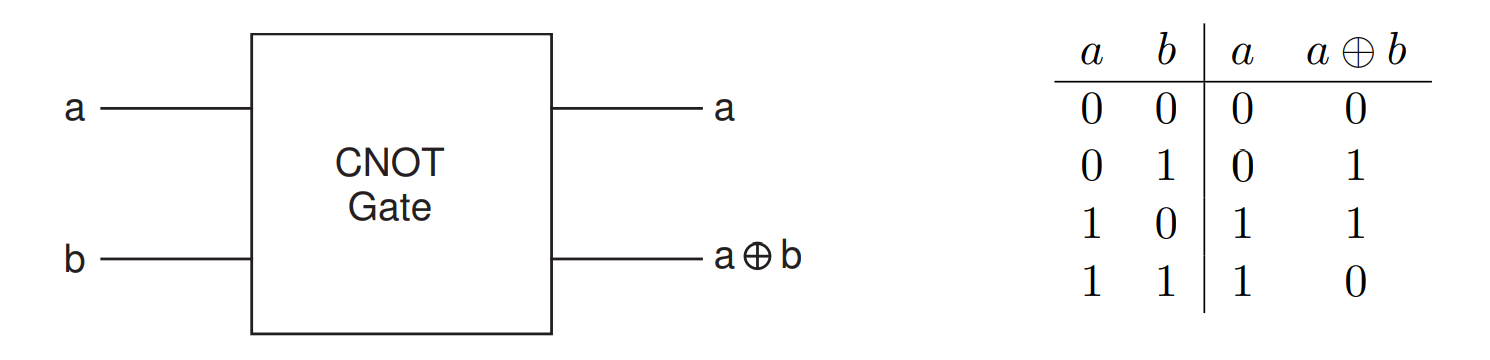
\includegraphics[scale=0.25]{cnot}
	\end{figure}
	Show by creating the truth table that the CNOT gate is reversible - that you can find
	the inputs if you know the outputs. In fact, you can show that CNOT is its own inverse.
	To do this you will ``prove'' the identity $a \oplus (a \oplus b) = b$.

	
	\item \textit{Toffoli Gate}. While the CNOT gate is reversible, it is not universal. That is, you cannot
	implement every possible logic operation with the CNOT. The NAND gate is actually
	\textit{universal}: you can create any logical operation using just NAND gates (but of course
	it isn’t reversible). In 1980 Tommaso Toffoli (MIT) described a universal reversible
	gate – now called the Toffoli gate or sometimes the ``controlled-controlled-not.'' [There’s
	another universal reversible gate called the Fredkin gate (or ``controlled-swap'') named
	after its inventor Edward Fredkin.] The Toffoli gate has three inputs and three outputs
	and its behavior is shown in the circuit diagram shown below. The outputs are a copy
	of both inputs and the logical expression $c \oplus (a \land b)$.
	\begin{figure}[!htb]
		\centering
		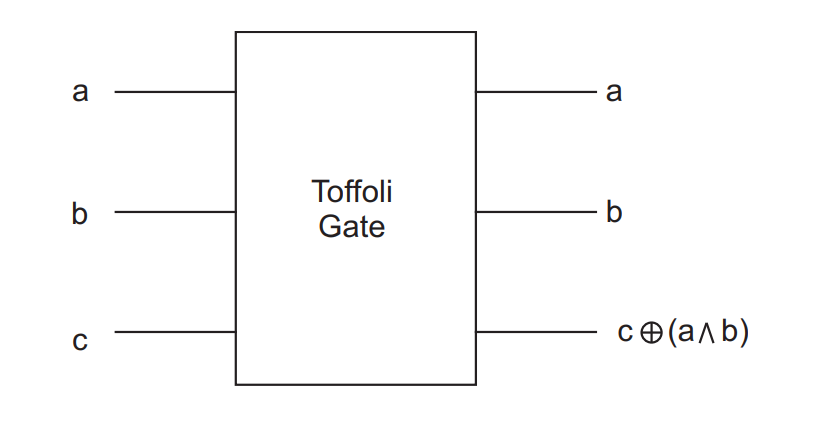
\includegraphics[scale=0.25]{toffoli}
	\end{figure}
	There are 8 possible input combinations to the Toffoli gate. Create a truth table for the
	Toffoli gate and show that for $c = 0$ that the output is $a \land b$ and for $c = 1$ that the output
	is $a \land b$ where $\land$ is the symbol for AND. That is, show the Toffoli gate can generate the
	same logical output as the AND or NAND gates.
	Show that the Toffoli gate is its own inverse by creating the truth table using the three
	outputs you calculated as inputs to a Toffoli gate.
	Why would the Toffoli gate be called the controlled-controlled-not (CCNOT)?
\end{enumerate}


\noindent \textit{Solution:} 
\begin{enumerate}[(a)]
	\item 
	$\,$CNOT:\\
	\begin{tabular}{| c  c |  c c| c| }
		\hline
		$a$ & $b$ & $a$ & $a\oplus b$  & $a\oplus(a\oplus b)$ \\
		\hline
		0&0&0&0&0\\
		0&1&0&1&1\\
		1&0&1&1&0\\
		1&1&1&0&1\\
		\hline
	\end{tabular}

	We have just shown (by exhaustion) that $a\oplus(a\oplus b) = b$, which means we can invert the CNOT gate to obtain its input $(a,b)$ for any given output $(a,a\oplus b)$. 
	
	\item 
	$\,$Toffoli:\\
	\begin{tabular}{| c  c  c  c| c c c| }
		\hline
		$a$ & $b$ & $c$ & $(a\land b)$ & $a$ & $b$&  $c\oplus (a\land b)$ \\
		\hline
		0&0&0&0&0&0&0\\
		0&0&1&0&0&0&1\\
		0&1&0&0&0&1&0\\
		0&1&1&0&0&1&1\\
		1&0&0&0&1&0&0\\
		1&0&1&0&1&0&1\\
		1&1&0&1&1&1&1\\
		1&1&1&1&1&1&0\\
		\hline
	\end{tabular}

	We see that $\text{Toff}[a,b,0]=a\land b$, and $\text{Toff}[a,b,1] = \overline{a\land b}$. So, by setting $c$ to be $0$ or $1$, we can make the Toffoli gate an AND or a NAND gate. \\
	
	To show that the Toffoli gate is its own inverse, we show $c = (a\land b) \oplus c\oplus (a\land b)$, once again by exhaustion:\\
	
	\begin{tabular}{| c  c  c  c| c c c| c |}
		\hline
		$a$ & $b$ & $c$ & $(a\land b)$ & $a$ & $b$&  $c\oplus (a\land b)$ & $(a\land b) \oplus c\oplus (a\land b)$  \\
		\hline
		0&0&0&0&0&0&0&0\\
		0&0&1&0&0&0&1&1\\
		0&1&0&0&0&1&0&0\\
		0&1&1&0&0&1&1&1\\
		1&0&0&0&1&0&0&0\\
		1&0&1&0&1&0&1&1\\
		1&1&0&1&1&1&1&0\\
		1&1&1&1&1&1&0&1\\
		\hline
	\end{tabular}

	The Toffoli gate would be called the controlled-controlled-not because unlike the CNOT where there is one control bit and one target bit, the Toffoli gate has \textbf{two} control bits, namely $a$ and $b$, and one target bit, namely $c$. The Toffoli gate flips $c$ if and only if $a = b = 1$. 
	
\end{enumerate}


\qed


\newpage
\noindent \textbf{3.} In Section 1.4, Mermin defines several 1-Cbit operations that do not correspond to any physical operation but which can be useful in deriving relationships between operations that do
have a physical meaning. The first two of these operators are the ``projection operators.'' 

\begin{figure}[!htb]
	\centering
	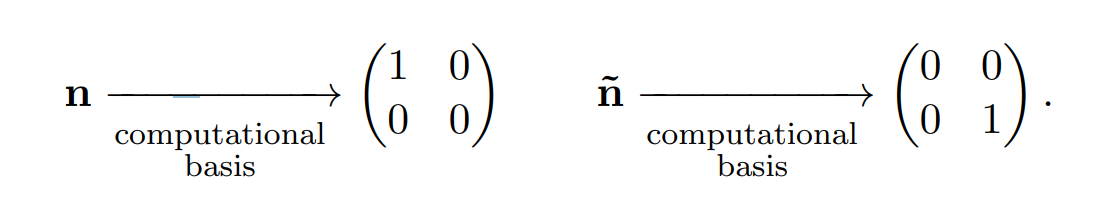
\includegraphics[scale=0.3]{proj}
\end{figure}
\begin{enumerate}[(a)]
	\item Show, using their matrix form, that as Mermin states on the top of page 12, the two
	matrices have eigenvalues of 0 and +1. Determine eigenvectors of each matrix assuming
	that they are in the form of probabilistic CBits
	\begin{align*}
	\ket{a} = \begin{pmatrix}
	a_0 \\ a_1
	\end{pmatrix}
	\end{align*}
	where the convention of probability requires $a_0 + a_1 = 1$. 
	
	\item Show, using the definitions, that the properties of Eq. 1.33 and 1.34 are correct.
	
\end{enumerate}


\noindent \textit{Solution:} 
\begin{enumerate}[(a)]
	\item Because $\mathbf{n}$ and $\tilde{\mathbf{n}}$ are diagonal matrices with only entries $0$ and $1$ along the diagonals, their eigenvalues are 0 and 1. \\
	
	The (stochastic) 1-eigenvector of $\mathbf{n}$, say $\ket{a}_1= (a_0\,\,a_1)^\top$ where $a_0 + a_1 = 1$, must be ${\ket{a}_1 = (1\,\,0)^\top}$ because $\mathbf{n}(a_0\,\,a_1)^\top = (a_0\,\,0)^\top$. By a similar argument, the (stochastic) 0-eigenvector of $\mathbf{n}$ must be ${\ket{a}_0 = (0\,\,1)^\top}$. By symmetry, the 1-eigenvector of $\tilde{\mathbf{n}}$ is ${\ket{\tilde{a}}_{{1}} = (0\,\,1)^\top}$, and the 0-eigenvector of $\tilde{\mathbf{n}}$ is ${\ket{\tilde{a}}_{{0}} = (1\,\,0)^\top}$.
	
	\item We note that projections are \textit{idempotents}, so $\mathbf{n}^2 = \mathbf{n}$ and $\tilde{\mathbf{n}}^2 = \tilde{\mathbf{n}}$ automatically. Next, because the images of $\mathbf{n}$ and $\tilde{\mathbf{n}}$ are orthogonal spaces (spanned by $(1\,\,0)^\top$ and $(0\,\,1)^\top$, respectively), $\mathbf{n}\tilde{\mathbf{n}} = \tilde{\mathbf{n}}\mathbf{n} = \mathbf{0}_{2\times 2}$. Finally, $\mathbf{n} + \tilde{\mathbf{n}} = \Id$ because the idempotents $\mathbf{n}$ and $\tilde{\mathbf{n}}$ \textit{resolve identity} $\Id$. \\
	
	We can also verify these properties algebraically:
	\begin{align}
	&\mathbf{n}^2 = \begin{pmatrix}
	1&0\\0&0
	\end{pmatrix}\begin{pmatrix}
	1&0\\0&0
	\end{pmatrix} = \begin{pmatrix}
	1&0\\0&0
	\end{pmatrix}\\
	&\tilde{\mathbf{n}}^2 = \begin{pmatrix}
	0&0\\0&1
	\end{pmatrix}\begin{pmatrix}
	0&0\\0&1
	\end{pmatrix}=\begin{pmatrix}
	0&0\\0&1
	\end{pmatrix}\\
	&\mathbf{n}\tilde{\mathbf{n}}= \begin{pmatrix}
	1&0\\0&0
	\end{pmatrix}
	\begin{pmatrix}
	0&0\\0&1
	\end{pmatrix} = \begin{pmatrix}
	0&0\\0&0
	\end{pmatrix} = \begin{pmatrix}
	0&0\\0&1
	\end{pmatrix}\begin{pmatrix}
	1&0\\0&0
	\end{pmatrix} = \tilde{\mathbf{n}}\mathbf{n}\\
	&\mathbf{n} +  \tilde{\mathbf{n}}  = \begin{pmatrix}
	1&0\\0&0
	\end{pmatrix} + \begin{pmatrix}
	0&0\\0&1
	\end{pmatrix} = \begin{pmatrix}
	1&0\\0&1
	\end{pmatrix} = \Id
	\end{align} 
	
	Next we consider the $\X = \begin{pmatrix}
	0&1\\1&0
	\end{pmatrix}$, the bit-flip:
	\begin{align}
	&\mathbf{n}\X = \begin{pmatrix}
	1&0\\0&0
	\end{pmatrix}\begin{pmatrix}
	0&1\\1&0
	\end{pmatrix}= \begin{pmatrix}
	0&1\\0&0
	\end{pmatrix}=\begin{pmatrix}
	0&1\\1&0
	\end{pmatrix}\begin{pmatrix}
	0&0\\0&1
	\end{pmatrix} = \mathbf{X}\tilde{\mathbf{n}}\\
	&\tilde{\mathbf{n}}\X = \begin{pmatrix}
	0&0\\0&1
	\end{pmatrix}\begin{pmatrix}
	0&1\\1&0
	\end{pmatrix}= \begin{pmatrix}
	0&0\\1&0
	\end{pmatrix}=\begin{pmatrix}
	0&1\\1&0
	\end{pmatrix}\begin{pmatrix}
	1&0\\0&0
	\end{pmatrix} = \mathbf{X}{\mathbf{n}}.
	\end{align}
	Mermin explained why this makes sense, so I won't repeat that.
	
	
\end{enumerate}

\qed













\newpage
\noindent \textbf{4.} Another pair of operators which do not have physical meaning when acting on CBits are the
``phase-flip operator'' $\mathbf{Z}$ and Hadamard operator $\had$. 
\begin{figure}[!htb]
	\centering
	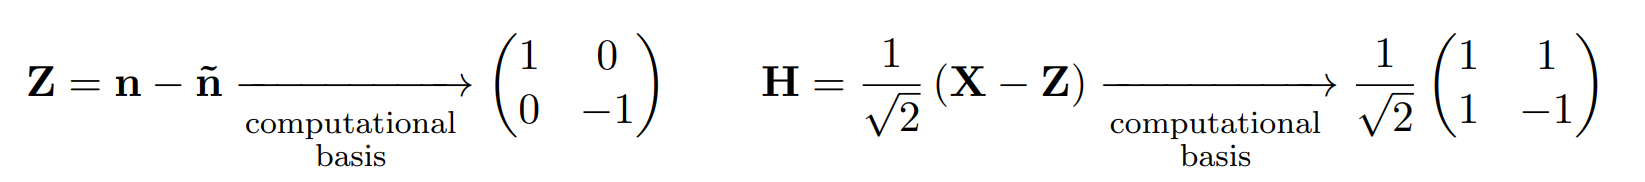
\includegraphics[scale=0.26]{ZH}
\end{figure}
where $\X$ is the ``bit-flip'' (NOT) operator. Both $\mathbf{Z}$ and $\had$ will be used and do have meaning when applied to QBits.

\begin{enumerate}[(a)]
	\item Show, using their matrix forms, that the three single-bit gates $\X$, $\mathbf{Z}$, and $\had$ are their
	own inverse. That is, show that $\X^2 = \Id$, $\mathbf{Z}^2 = \Id$, and $\had^2 = \Id$.
	\item Show, using their matrix forms, that the identities of Eq. 1.43 are correct. That is, show
	that using a Hadamard gate to perform a ``similarity transformation'' you can convert a bit-flip to a phase-flip and vice-versa.
\end{enumerate}

\noindent \textit{Solution:} 

\begin{enumerate}[(a)]
	\item 
	\begin{align}
	\mathbf{Z}^2 &= \begin{pmatrix}
	1&0\\0&-1
	\end{pmatrix}\begin{pmatrix}
	1&0\\0&-1
	\end{pmatrix} = \begin{pmatrix}
	1&0\\0&1
	\end{pmatrix}\\
	\X^2 &= \begin{pmatrix}
	0&1\\1&0
	\end{pmatrix}\begin{pmatrix}
	0&1\\1&0
	\end{pmatrix} = \begin{pmatrix}
	1&0\\0&1
	\end{pmatrix}\\
	\had^2 &= \f{1}{2}\begin{pmatrix}
	1&1\\1&-1
	\end{pmatrix}\begin{pmatrix}
	1&1\\1&-1
	\end{pmatrix} = \begin{pmatrix}
	1&0\\0&1
	\end{pmatrix}.
	\end{align}
	
	\item 
	\begin{align}
	\had \X \had &= \f{1}{2}\begin{pmatrix}
	1&1\\1&-1
	\end{pmatrix}\begin{pmatrix}
	0&1\\1&0
	\end{pmatrix}\begin{pmatrix}
	1&1\\1&-1
	\end{pmatrix} = \begin{pmatrix}
	1&0\\0&-1
	\end{pmatrix} = \mathbf{Z}\\
	\had \X\had &= \mathbf{Z} \implies \X = \had^{-1}\mathbf{Z}\had^{-1}  \implies \X = \had \mathbf{Z} \had \quad (\had^{-1} = \had) 
	\end{align}
\end{enumerate}
\qed























\newpage



\section{Problem set 2}



\noindent \textbf{1.} Compute, using the matrix representations of the operators and probability-vector states, the result of applying a Hadamard transofmr to both bits of a two-Cbit state $\ket{ba} = \ket{b}\ket{a} = \ket{b}\otimes \ket{a}$ first by creating the tensor product of the two vectors $\had \ket{b}\otimes \had\ket{a}$ and second by creating the tensor product of the Hadamard operators $\had_1 \had_0 = \had \otimes \had$ and applying it to the state $\ket{b}\ket{a}$.\\



\noindent \textit{Solution:} The tensor product works the way we want it to work:
\begin{align}\label{first}
\had \ket{b} \otimes \had\ket{a} &= \f{1}{\sqrt{2}}\begin{pmatrix}
1 & 1 \\ 1 & -1
\end{pmatrix}\begin{pmatrix}
b_0 \\ b_1
\end{pmatrix}  \otimes \f{1}{\sqrt{2}}\begin{pmatrix}
1 & 1 \\ 1 & -1
\end{pmatrix}\begin{pmatrix}
a_0 \\ a_1
\end{pmatrix}  \nn\\
&= \f{1}{\sqrt{2}} \begin{pmatrix}
b_0 + b_1 \\ b_0 - b_1
\end{pmatrix} \otimes \f{1}{\sqrt{2}}\begin{pmatrix}
a_0 + a_1 \\ a_0 - a_1
\end{pmatrix} \nn\\
&= \f{1}{\sqrt{2}}\lb (b_0+b_1)\ket{0} + (b_0 - b_1)\ket{1} \rb \otimes \f{1}{\sqrt{2}}\lb (a_0+a_1)\ket{0} + (a_0 - a_1)\ket{1} \rb \nn\\
&= \f{1}{2}\lb (b_0+b_1)(a_0+a_1)\ket{00} + (b_0-b_1)(a_0+a_1)\ket{10}\right. \nn\\
&\left.\quad + (b_0+b_1)(a_0-a_1)\ket{01} + (b_0-b_1)(a_0-a_1)\ket{11} \rb.
\end{align}

\begin{align}\label{second}
(\had\otimes \had)\ket{ba} &= 
\f{1}{\sqrt{2}}\begin{pmatrix}
\f{1}{\sqrt{2}}\begin{pmatrix}
1 & 1 \\ 1 & -1
\end{pmatrix} & \f{1}{\sqrt{2}}\begin{pmatrix}
1 & 1 \\ 1 & -1
\end{pmatrix}\\
\f{1}{\sqrt{2}}\begin{pmatrix}
1 & 1 \\ 1 & -1
\end{pmatrix} & -\f{1}{\sqrt{2}}\begin{pmatrix}
1 & 1 \\ 1 & -1
\end{pmatrix}
\end{pmatrix}\begin{pmatrix}
b_0\begin{pmatrix}
a_0\\a_1
\end{pmatrix}\\
b_1\begin{pmatrix}
a_0\\a_1
\end{pmatrix}
\end{pmatrix} \nn\\
&= \f{1}{2}\begin{pmatrix}
1&1&1&1\\
1&-1&1&-1\\
1&1&-1&-1\\
1&-1&-1&1
\end{pmatrix}\begin{pmatrix}
b_0a_0\\b_0a_1\\b_1a_0\\b_1a_1
\end{pmatrix}\nn\\
&= \dots \text{(multiply in and factor)}\nn\\
&= \f{1}{2}\lb (b_0+b_1)(a_0+a_1)\ket{00} + (b_0-b_1)(a_0+a_1)\ket{10}\right. \nn\\
&\left.\quad + (b_0+b_1)(a_0-a_1)\ket{01} + (b_0-b_1)(a_0-a_1)\ket{11} \rb.
\end{align}
From Eq. \eqref{first} and \eqref{second}, 
\begin{align}
\boxed{\had \ket{b}\otimes \had \ket{a} = (\had\otimes \had)\ket{ba}}
\end{align}\qed




\newpage


\noindent \textbf{2.} Writing out the matrix representations, show that Mermin's identity $\mathbf{S}_{ij} = \mathbf{C}_{ij}\mathbf{C}_{ji}\mathbf{C}_{ij}$ is true for $\mathbf{S}_{ij}$.\\



\noindent \textit{Solution:} Let $i=0,j=1$, then 
\begin{align}
\mathbf{C}_{01}\mathbf{C}_{10}\mathbf{C}_{01} &= \begin{pmatrix}
1 &&&\\&&&1\\&&1&\\&1&&
\end{pmatrix}
\begin{pmatrix}
1&&&\\&1&&\\&&&1\\&&1&
\end{pmatrix}
\begin{pmatrix}
1 &&&\\&&&1\\&&1&\\&1&&
\end{pmatrix}\nn\\
&= \begin{pmatrix}
1 &&&\\&&&1\\&&1&\\&1&&
\end{pmatrix}
\begin{pmatrix}
1 &&&\\&&&1\\&1&&\\&&1&
\end{pmatrix}\nn\\
&= \begin{pmatrix}
1&&&\\&&1&\\&1&&\\&&&1
\end{pmatrix}\nn\\
&= \mathbf{S}_{10} = \mathbf{S}_{01}.
\end{align}
Let $i=1,j=0$, then
\begin{align}
\mathbf{C}_{10}\mathbf{C}_{01}\mathbf{C}_{01} &=
\begin{pmatrix}
1&&&\\&1&&\\&&&1\\&&1&
\end{pmatrix} \begin{pmatrix}
1 &&&\\&&&1\\&&1&\\&1&&
\end{pmatrix}
\begin{pmatrix}
1&&&\\&1&&\\&&&1\\&&1&
\end{pmatrix}\nn\\
&= \begin{pmatrix}
1&&&\\&1&&\\&&&1\\&&1&
\end{pmatrix}\begin{pmatrix}
1&&&\\&&&1\\&1&&\\&&1&
\end{pmatrix} \nn\\
&= \begin{pmatrix}
1&&&\\&&1&\\&1&&\\&&&1
\end{pmatrix}\nn\\
&=\mathbf{S}_{10} = \mathbf{S}_{01}.
\end{align}\qed


\newpage




\noindent \textbf{3.} Show, using matrix operations, that surrounding a CNOT with two Hadamard gates switches the role of the control-bit and target bit. Specifically, using the matrices show that $\mathbf{C}_{10} = (\had_0 \had_1)\mathbf{C}_{01}(\had_0\had_1)$, or formally that 
\begin{align}
\mathbf{C}_{10} = (\had \otimes \had) \mathbf{C}_{01} (\had \otimes \had).
\end{align}
This will demonstrate a special case  of 
\begin{align}
\mathbf{C}_{ji} = (\had_j \had_i) \mathbf{C}_{ij} (\had_i \had_j).
\end{align}



\noindent \textit{Solution:} 
\begin{align}
(\had \otimes \had) \mathbf{C}_{01} (\had \otimes \had) &=  \f{1}{4}\begin{pmatrix}
1&1&1&1\\
1&-1&1&-1\\
1&1&-1&-1\\
1&-1&-1&1
\end{pmatrix}\begin{pmatrix}
1 &&&\\&&&1\\&&1&\\&1&&
\end{pmatrix}\begin{pmatrix}
1&1&1&1\\
1&-1&1&-1\\
1&1&-1&-1\\
1&-1&-1&1
\end{pmatrix}\nn\\
&= \f{1}{4}\begin{pmatrix}
1&1&1&1\\
1&-1&1&-1\\
1&1&-1&-1\\
1&-1&-1&1
\end{pmatrix}\begin{pmatrix}
1& 1& 1& 1\\
1& -1& -1& 1\\
1& 1& -1& -1\\
1& -1& 1& -1
\end{pmatrix}\nn\\
&= \begin{pmatrix}
1&&&\\&1&&\\&&&1\\&&1&
\end{pmatrix} \nn\\
&= \mathbf{C}_{10}
\end{align}

Conversely,
\begin{align}
(\had \otimes \had) \mathbf{C}_{10} (\had \otimes \had) &=  \f{1}{4}\begin{pmatrix}
1&1&1&1\\
1&-1&1&-1\\
1&1&-1&-1\\
1&-1&-1&1
\end{pmatrix}\begin{pmatrix}
1 &&&\\&1&&\\&&&1\\&&1&
\end{pmatrix}\begin{pmatrix}
1&1&1&1\\
1&-1&1&-1\\
1&1&-1&-1\\
1&-1&-1&1
\end{pmatrix}\nn\\
&= \f{1}{4}\begin{pmatrix}
1&1&1&1\\
1&-1&1&-1\\
1&1&-1&-1\\
1&-1&-1&1
\end{pmatrix}\begin{pmatrix}
1& 1& 1& 1\\
1& -1& 1& -1\\
1& -1& -1& 1\\
1& 1& -1& -1
\end{pmatrix}\nn\\
&= \begin{pmatrix}
1&&&\\&&&1\\&&1&\\&1&&
\end{pmatrix} \nn\\
&= \mathbf{C}_{01}
\end{align}



\newpage



\noindent \textbf{4.} Following the examples in class of determining the matrices for the ``conditional operations'' $\mathbf{S}_{01} = \mathbf{S}_{10}, \mathbf{C}_{01}, \mathbf{C}_{10}, \mathbf{T}_{210}$ determine the $8\times 8$ matrix that represents the Toffoli gate $\mathbf{T}_{012}$, which uses Cbits 0 and 1 as the control bits and Cbits 2 as the target bit. 
\begin{align}
\mathbf{T}_{012}\ket{c}\ket{b}\ket{a} = \ket{c\oplus (a\land b)}\ket{b}\ket{a}.
\end{align}



\noindent \textit{Solution:} Truth table for $\mathbf{T}_{012}$:\\
	
	
\begin{tabular}{| c  c  c  c| c c c| }
	\hline
	$c$ & $b$ & $a$ & $(a\land b)$ & $c\oplus(a\land b)$ & $b$&  $a$ \\
	\hline
	0&0&0&0&0&0&0\\
	0&0&1&0&0&0&1\\
	0&1&0&0&0&1&0\\
	0&1&1&1&1&1&1\\
	1&0&0&0&1&0&0\\
	1&0&1&0&1&0&1\\
	1&1&0&0&1&1&0\\
	1&1&1&1&0&1&1\\
	\hline
\end{tabular}\\




We see that $\mathbf{T}_{012}$ acts as identity for all states except for some cases:
\begin{align}
&\mathbf{T}_{012}\ket{011} = \ket{111}\\
&\mathbf{T}_{012}\ket{111} = \ket{011},
\end{align}
as expected. These correspond to two off-diagonal indices in the matrix for $\mathbf{T}_{012}$. Based on the $\mathbf{T}_{210}$ matrix:
\begin{align}
\begin{blockarray}{ccccccccc}
\ket{000} & \ket{001} & \ket{010} & \ket{011} & \ket{100} & \ket{101}& \ket{110} & \ket{111} \\
\begin{block}{(cccccccc)c}
1 & 0 & 0 & 0 & 0 & 0 & 0 & 0 & \ket{000} \\
0 & 1 & 0 & 0 & 0 & 0 & 0 & 0 & \ket{001} \\
0 & 0 & 1 & 0 & 0 & 0 & 0 & 0 & \ket{010} \\
0 & 0 & 0 & 1 & 0 & 0 & 0 & 0 & \ket{011} \\
0 & 0 & 0 & 0 & 1 & 0 & 0 & 0 & \ket{100} \\
0 & 0 & 0 & 0 & 0 & 1 & 0 & 0 & \ket{101} \\
0 & 0 & 0 & 0 & 0 & 0 & 0 & 1 & \ket{110} \\
0 & 0 & 0 & 0 & 0 & 0 & 1 & 0 & \ket{111} \\
\end{block}
\end{blockarray}
\end{align}

By analogy, the matrix for $\mathbf{T}_{012}$ is:
\begin{align}
\begin{blockarray}{ccccccccc}
\ket{000} & \ket{001} & \ket{010} & \ket{011} & \ket{100} & \ket{101}& \ket{110} & \ket{111} \\
\begin{block}{(cccccccc)c}
1 & 0 & 0 & 0 & 0 & 0 & 0 & 0 & \ket{000} \\
0 & 1 & 0 & 0 & 0 & 0 & 0 & 0 & \ket{001} \\
0 & 0 & 1 & 0 & 0 & 0 & 0 & 0 & \ket{010} \\
0 & 0 & 0 & 0 & 0 & 0 & 0 & 1 & \ket{011} \\
0 & 0 & 0 & 0 & 1 & 0 & 0 & 0 & \ket{100} \\
0 & 0 & 0 & 0 & 0 & 1 & 0 & 0 & \ket{101} \\
0 & 0 & 0 & 0 & 0 & 0 & 1 & 0 & \ket{110} \\
0 & 0 & 0 & 1 & 0 & 0 & 0 & 0 & \ket{111} \\
\end{block}
\end{blockarray}
\end{align}






\newpage



\section{Problem set 3}


\noindent \textbf{1.} With 
\begin{align}
\mathbf{S}_{ij} = \n_i\n_j + \tilde{\mathbf{\n}}_i \tilde{\mathbf{\n}}_j + \X_i\X_j(\n_i\tilde{\mathbf{n}}_j + \tilde{\mathbf{n}}_i \n_j)
\end{align}
and the identities
\begin{align}
\n^2 = \n, \quad \tilde{\n}^2 = \tilde{\mathbf{n}}, \quad \n\tilde{\n} = \tilde{\n}\n = \mathbf{0}, \quad \tilde{\n}+{\n} = \Id, \nn\\
\X^2 = \Id, \quad \n\X = \X \tilde{\n}, \quad \tilde{\n}\X = \X \n
\end{align}
show that 
\begin{align}
\mathbf{S}_{ij}^2 = \Id.
\end{align}


\noindent \textit{Solution:} We will extensively use the fact that $[\mathbf{P}_i,\mathbf{Q}_j] = 0$. The strategy here is to make the $\X_i$'s and $\X_j$'s combine and let $\tilde{\n}$ and $\n$ annihilate each other as many times as possible:
\begin{align}
\mathbf{S}_{ij}^2 &= \lb \n_i\n_j + \tilde{\mathbf{\n}}_i \tilde{\mathbf{\n}}_j + \X_i\X_j(\n_i\tilde{\mathbf{n}}_j + \tilde{\mathbf{n}}_i \n_j) \rb^2\nn\\
&= \n_i\n_j\n_i\n_j + \tilde{\mathbf{\n}}_i \tilde{\mathbf{\n}}_j\tilde{\mathbf{\n}}_i \tilde{\mathbf{\n}}_j + \X_i\X_j(\n_i\tilde{\mathbf{n}}_j + \tilde{\mathbf{n}}_i \n_j)\X_i\X_j(\n_i\tilde{\mathbf{n}}_j + \tilde{\mathbf{n}}_i \n_j) \nn\\
&\quad +\cancel{\n_i\n_j\tilde{\mathbf{\n}}_i \tilde{\mathbf{\n}}_j} + {\tilde{\mathbf{\n}}_i \tilde{\mathbf{\n}}_j\X_i\X_j(\n_i\tilde{\mathbf{n}}_j + \tilde{\mathbf{n}}_i \n_j)} + \cancel{\X_i\X_j(\n_i\tilde{\mathbf{n}}_j + \tilde{\mathbf{n}}_i \n_j)\n_i\n_j} \nn\\
&\quad +\cancel{\tilde{\mathbf{\n}}_i \tilde{\mathbf{\n}}_j\n_i\n_j} + \cancel{\X_i\X_j(\n_i\tilde{\mathbf{n}}_j + \tilde{\mathbf{n}}_i \n_j)\tilde{\mathbf{\n}}_i \tilde{\mathbf{\n}}_j} + \cancel{\n_i\n_j\X_i\X_j(\n_i\tilde{\mathbf{n}}_j + \tilde{\mathbf{n}}_i \n_j)}\nn\\
&= \n_i \n_j + \tilde{\n}_i\tilde{\n}_j +  (\tilde{\n}_i\n_j+\n_i\tilde{\n}_j)\underbrace{\X_i^2\X_j^2}_{\Id_4}(\n_i\tilde{\n}_j+\tilde{\n}_i\n_j) \nn\\ &\quad +\cancel{\X_i\X_j\n_i\n_j(\n_i\tilde{\mathbf{n}}_j + \tilde{\mathbf{n}}_i \n_j)}\nn\\
&= \n_i \n_j + \tilde{\n}_i\tilde{\n}_j + \mathbf{0} + \tilde{\n}_i\n_j + \n_i\tilde{\n}_j + \mathbf{0}\nn\\
&= \n_i(\n_j+ \tilde{\n}_j) + \n_j(\n_j + \tilde{\n}_j)\nn\\
&= \n_i\Id_j + \tilde{\n}_i \Id_j \nn\\
&= \Id_i \otimes \Id_j \nn\\
&\equiv \Id.
\end{align}
\qed



\newpage





\noindent \textbf{2.} With
\begin{align}
\mathbf{S}_{ij} = \mathbf{C}_{ij}\mathbf{C}_{ji}\mathbf{C}_{ij}
\end{align}
and 
\begin{align}
\mathbf{C}_{ij} = \tilde{\n}_i\Id_j + \n_i \X_j
\end{align}
and other identities show that
\begin{align}
\mathbf{S}_{ij} = \n_i\n_j + \tilde{\mathbf{\n}}_i \tilde{\mathbf{\n}}_j + \X_i\X_j(\n_i\tilde{\mathbf{n}}_j + \tilde{\mathbf{n}}_i \n_j)
\end{align}


\noindent \textit{Solution:} We can create a lot of cancellations using the identities $\n\X = \X \tilde{\n}$ and $\tilde{\n}\X = \X\n$. Also, because $\tilde{\n}$ and $\n$ are idempotents, they are the same as their powers (except power 0). With this, we can ``merge'' and simplify a lot of the summands. 
\begin{align}
\mathbf{S}_{ij} &= \mathbf{C}_{ij}\mathbf{C}_{ji}\mathbf{C}_{ij}\nn\\
&= [\tilde{\n}_i\Id_j + \n_i \X_j][\tilde{\n}_j\Id_i + \n_j \X_i][\tilde{\n}_i\Id_j + \n_i \X_j]\nn\\
&= [\tilde{\n}_i\Id_j + \n_i \X_j][\tilde{\n}_i \tilde{\n}_j + \n_i \X_j \n_j +  \X_i \tilde{\n}_i \n_j + \X_i\X_j{\n}_i\tilde{\n}_j]\nn\\
&= \tilde{\n}_i\tilde{\n}_j + \X_i\X_j {\n}_i\tilde{\n}_j + \n_i\n_j +  \X_i\X_j\tilde{\n}_i{\n}_j + \text{cancellations}\nn\\
&= \n_i\n_j + \tilde{\mathbf{\n}}_i \tilde{\mathbf{\n}}_j + \X_i\X_j(\n_i\tilde{\mathbf{n}}_j + \tilde{\mathbf{n}}_i \n_j).
\end{align}
The cancellations are exactly those where $\tilde{\n}$ and $\n$ annihilate each other. Some are obvious; some are found by using the identities $\n\X = \X \tilde{\n}$ and $\tilde{\n}\X = \X\n$ to ``bring the $\tilde{\n}$ and $\n$ together for \textit{mutual annihilation}.''
\qed





\newpage


\noindent \textbf{3.} With  
\begin{align}
\mathbf{C}_{ij} = \f{1}{2}\lb (\Id_i + \Z_i)\Id_j + (\Id_i - \Z_i)\X_j \rb
\end{align}
and
\begin{align}
\had \X \had = \Z \quad \had \Z \had = \X \quad \had^2 =\Id
\end{align}
and other identities show that
\begin{align}
\mathbf{C}_{ji} = (\had_i \had_j)\mathbf{C}_{ij}(\had_i\had_j)
\end{align}



\noindent \textit{Solution:} It is easier to go from the RHS to the LHS, using the identities above:
\begin{align}
(\had_i \had_j)\mathbf{C}_{ij}(\had_i\had_j) &= (\had_i \had_j)\lb \f{1}{2}\lb (\Id_i + \Z_i)\Id_j + (\Id_i - \Z_i)\X_j \rb  \rb(\had_i\had_j)\nn\\
&= \f{1}{2}\lb \had_i^2\had_j^2 + \X_i \had_j^2 +  \had_i^2 \Z_j - (\had_i\Z_i\had_i)(\had_j\X_j\had_j) \rb\nn\\
&= \f{1}{2}\lb (\Id_i + \Z_i)\Id_j + \Id_j \X_i - \X_i \Z_j \rb\nn\\
&= \f{1}{2}\lb (\Id_j + \Z_j)\Id_i + (\Id_j - \Z_j)\Id_i  \rb\nn\\
&\equiv \mathbf{C}_{ji}.
\end{align}\qed






\newpage



\noindent \textbf{4.} Suppose you have been sent a set of photons, and you measure the polarization using a PBS. For each of the states, determine the probability for measuring the photon being in states $\ket{0} = \ket{x}$ and $\ket{1} = \ket{y}$. 
\begin{enumerate}[(a)]
	\item $\f{1}{\sqrt{3}}\ket{0} + \sqrt{\f{2}{3}}\ket{1}$
	\item $\f{1}{\sqrt{2}}(\ket{+45} + \ket{-45} ) $
	\item $\f{1}{\sqrt{2}}(\ket{+45} - \ket{-45}) $
	\item $\f{1}{\sqrt{2}}(\ket{R} - \ket{L})$
	\item $\f{\sqrt{3}}{2}\ket{R} + \f{1}{2}\ket{L}$
\end{enumerate}


\noindent \textit{Solution:} 
\begin{enumerate}[(a)]
	\item $P(\ket{0}) = 1/3, P(\ket{1}) = {2/3}$.
	\item The given state can be rewritten in the $0-1$ basis:
	\begin{align}
	\f{1}{\sqrt{2}}(\ket{+45} + \ket{-45} ) \equiv \ket{0}
	\end{align}
	so that $P(\ket{0}) = 1, P(\ket{1}) = 0$.
	\item The given state can be rewritten in the $0-1$ basis:
	\begin{align}
	\f{1}{\sqrt{2}}(\ket{+45} - \ket{-45}) = \ket{1}
	\end{align}
	so that $P(\ket{0}) = 0, P(\ket{1}) = 1$.
	\item The given state can be rewritten in the $0-1$ basis:
	\begin{align}
	\f{1}{\sqrt{2}}(\ket{R} - \ket{L}) = \f{1}{2}\begin{pmatrix}
	0 \\ 2i
	\end{pmatrix} = i\begin{pmatrix}
	0\\1
	\end{pmatrix} = i\ket{1}
	\end{align}
	so $P(\ket{0}) = 0, P(\ket{1}) = 1$.
	\item The given state can be rewritten in the $0-1$ basis as
	\begin{align}
	\f{\sqrt{3}}{2}\ket{R} + \f{1}{2}\ket{L} = \f{1}{2\sqrt{2}}\begin{pmatrix}
	\sqrt{3}+1 \\ i(\sqrt{3}-1)
	\end{pmatrix}
	\end{align}
	so that $P(\ket{0}) = \abs{\f{\sqrt{3}+1}{2\sqrt{2}}}^2 \approx 0.933, P(\ket{1}) = \abs{\f{i(\sqrt{3}-1)}{2\sqrt{2}}}^2 \approx 0.067$.
\end{enumerate}\qed




\newpage















\noindent \textbf{5.} A rotation operator $\mathbf{R}_\phi$ on photons is one that takes a photon linearly polarized at angle $\alpha$ and converts it into a linearly polarized photon at angle $\al+\phi$. A matrix representation of the rotation operator in the computation basis is
\begin{align}
\mathbf{R}_\phi = \begin{pmatrix}
\cos\phi & -\sin\phi \\ \sin\phi & \cos\phi
\end{pmatrix}
\end{align}
\begin{enumerate}[(a)]
	\item Show that $\mathbf{R}_\phi$ is unitary.
	\item Show that $\mathbf{R}_\phi\ket{0} = \ket{\phi}$ and $\mathbf{R}_\phi \ket{1} = \ket{\pi/2+ \phi}$
	\item Show that $\mathbf{R}_\phi \ket{\al} = \ket{\al + \phi}$, where $\ket{\al} = \ket{\epsilon_{\alpha,0}}$
	\item Show that $\mathbf{R}_\phi$ acting on a right-handed photon $\mathbf{R}_\phi\ket{R}$ gives you back a right handed photon with an overall phase shift $\phi$.
	\item Show that the sequence of three operators $\mathbf{R}_{\phi}\Z \mathbf{R}_{-\phi}$ on a photon in the state $\ket{\epsilon}$ is equivalent to the Hadamard gate if $\phi = \pi/8$. To do this you just need to show that $\mathbf{R}_{-\phi}\Z \mathbf{R}_\phi = \had$ when $\phi = \pi/8$. 
\end{enumerate}










\noindent \textit{Solution:} 
\begin{enumerate}[(a)]
	\item By inspection, $\mathbf{R}_\phi$ is orthogonal, so it is unitary. Explicitly,
	\begin{align}
	\mathbf{R}_\phi^\dagger \mathbf{R}_\phi = 
	\begin{pmatrix}
	\cos\phi & \sin\phi \\ -\sin\phi & \cos\phi
	\end{pmatrix}
	\begin{pmatrix}
	\cos\phi & -\sin\phi \\ \sin\phi & \cos\phi
	\end{pmatrix} = \Id_{2\times 2}.
	\end{align}
	$\mathbf{R}_\phi^\dagger \mathbf{R}_\phi$ is simply a rotation by $\phi$, followed by a rotation by $-\phi$, so the composition is the identity function.
	
	\item 
	\begin{align}
	\mathbf{R}_\phi\ket{0} &= \begin{pmatrix}
	\cos\phi & -\sin\phi \\ \sin\phi & \cos\phi
	\end{pmatrix}\begin{pmatrix}
	1\\0
	\end{pmatrix} = \begin{pmatrix}
	\cos\phi \\ \sin\phi
	\end{pmatrix} = \ket{\phi}\\
	\mathbf{R}_\phi\ket{1} &= \begin{pmatrix}
	\cos\phi & -\sin\phi \\ \sin\phi & \cos\phi
	\end{pmatrix}\begin{pmatrix}
	0\\1
	\end{pmatrix} \nn\\
	&= \begin{pmatrix}
	-\sin\phi \\ \cos\phi
	\end{pmatrix} = \begin{pmatrix}
	\cos(\pi/2+\phi) \\ \sin(\pi/2+\phi)
	\end{pmatrix} = \ket{\pi/2 + \phi}.
	\end{align}
	$\mathbf{R}_\phi$ is a rotation by $\phi$, so starting at $\ket{0}$ and $\ket{1}\equiv \ket{\pi/2}$ give $\ket{\phi}$ and $\ket{\pi/2+\phi}$, respectively.
	
	\item 
	\begin{align}
	\mathbf{R}_\phi\ket{\al} &=  \begin{pmatrix}
	\cos\phi & -\sin\phi \\ \sin\phi & \cos\phi
	\end{pmatrix}\begin{pmatrix}
	\cos\al \\ \sin\al
	\end{pmatrix}\nn\\
	&= \begin{pmatrix}
	\cos\phi \cos\al - \sin\phi\sin\al \\
	\sin\phi \cos\al + \cos\phi \sin\al
	\end{pmatrix} = \begin{pmatrix}
	\cos(\al+\phi)\\\sin(\al+\phi)
	\end{pmatrix} = \ket{\al + \phi}.
	\end{align}
	$\ket{\al}$ can also be written in the $\ket{0}, \ket{1}$ basis states. By linearity, each is rotated by $\phi$, so $\ket{\al}$ becomes $\ket{\al + \phi}$.
	
	\item 
	\begin{align}
	\mathbf{R}_\phi \ket{R} = \begin{pmatrix}
	\cos\phi & -\sin\phi \\ \sin\phi & \cos\phi
	\end{pmatrix}\f{1}{\sqrt{2}}\begin{pmatrix}
	1\\i
	\end{pmatrix} = \f{1}{\sqrt{2}}\begin{pmatrix}
	e^{-i\phi}\\ie^{-i\phi}
	\end{pmatrix} = e^{-i\phi}\ket{R}.
	\end{align}
	The Euler identity allows us to factor out the phase shift factor.
	
	\item When $\phi = \pi/8$,
	\begin{align}
	\mathbf{R}_{\pi/8}\Z \mathbf{R}_{-\pi/8} &= \begin{pmatrix}
	\cos\phi & \sin\phi \\ -\sin\phi & \cos\phi
	\end{pmatrix}\begin{pmatrix}
	0&1\\1&0
	\end{pmatrix}\begin{pmatrix}
	\cos\phi & -\sin\phi \\ \sin\phi & \cos\phi
	\end{pmatrix}\bigg\vert_{\phi = \pi/8}\nn\\
	&= \begin{pmatrix}
	\cos\phi & \sin\phi \\ -\sin\phi & \cos\phi
	\end{pmatrix}\begin{pmatrix}
	\sin\phi & \cos\phi \\ \cos\phi & -\sin\phi
	\end{pmatrix}\bigg\vert_{\phi = \pi/8}\nn\\
	&= \begin{pmatrix}
	\sin(2\phi) &  \cos(2\phi)  \\ \cos(2\phi) & -\sin(2\phi)
	\end{pmatrix}\bigg\vert_{\pi/8}\nn\\
	&= \f{1}{\sqrt{2}}\begin{pmatrix}
	1 & 1 \\ 1 & -1
	\end{pmatrix} \equiv \had.
	\end{align}
\end{enumerate}\qed





















\newpage



\section{Problem set 4}


\noindent \textbf{1. Measurements.} Consider measurements of the two-Qbit states
\begin{align}
&\ket{\psi}_2 = \ket{+}\ket{-}\nn\\
&\ket{\phi}_2 = \f{1}{\sqrt{2}}\lp \ket{0}\ket{+} - \ket{1}\ket{-} \rp\nn\\
&\ket{\chi}_2 = \f{1}{\sqrt{2}}\lp \ket{+}\ket{+} + \ket{-}\ket{-} \rp\nn
\end{align} 
\begin{enumerate}[(a)]
	\item Write out the states in Dirac notation as
	\begin{align}
	&\ket{\psi}_2 = \sum_{0\leq x < 2^2} \psi_x \ket{x} \nn\\
	&\ket{\phi}_2 = \sum_{0 \leq x < 2^2} \phi_x \ket{x}  \nn\\
	&\ket{\chi}_2 = \sum_{0 \leq x < 2^2} \chi_x \ket{x} \nn
	\end{align}
	for $x \in \{ 0,1\}^2$. 
	\item  For each state $\ket{\psi}$, $\ket{\phi}$, and $\ket{\chi}$, what is the probability of finding the system in each of
	the four different states $\ket{x}$?
	\item  Which, if any, of these states are entangled? Explain.

\end{enumerate}



\noindent \textit{Solution:} 


\begin{enumerate}[(a)]
	\item We use the identities:
	\begin{align}
	\ket{+} = \f{1}{\sqrt{2}}\lp \ket{0} + \ket{1} \rp, \quad \text{and} \quad \ket{-} = \f{1}{\sqrt{2}}\lp \ket{0} - \ket{1} \rp
	\end{align}
	to write
	\begin{align}
	\ket{\psi}_2 
	&= \f{1}{2}\lp \ket{0} + \ket{1}  \rp\lp \ket{0} - \ket{1}  \rp\nn\\
	&= \f{1}{2}\lp \ket{00} + \ket{01} - \ket{10}- \ket{11} \rp\nn\\
	&= \boxed{\f{1}{2}\ket{0}_2 + \f{1}{2}\ket{1}_2 - \f{1}{2}\ket{2}_2 - \f{1}{2}\ket{3}_2}
	\end{align}
	\begin{align}
	\ket{\phi}_2 
	&= \f{1}{2}\lp \ket{0}\lb \ket{0} + \ket{1} \rb - \ket{1}\lb \ket{0} - \ket{1} \rb \rp\nn\\
	&= \f{1}{2}\lp \ket{00} + \ket{01} - \ket{10} + \ket{11} \rp\nn\\
	&= \boxed{\f{1}{2}\ket{0}_2 + \f{1}{2}\ket{1}_2 - \f{1}{2}\ket{2}_2 + \f{1}{2}\ket{3}_2}
	\end{align}
	\begin{align}
	\ket{\chi}_2 
	&= \f{1}{2\sqrt{2}}\lp \lb \ket{0} + \ket{1} \rb \lb \ket{0} + \ket{1} \rb + \lb \ket{0} - \ket{1} \rb \lb \ket{0} - \ket{1} \rb  \rp\nn\\
	&= \f{1}{2\sqrt{2}}\lp  \ket{00} + \ket{11} + \ket{00} + \ket{11} \rp\nn\\
	&= \f{1}{\sqrt{2}}\lp \ket{00} + \ket{11} \rp\nn\\
	&= \boxed{\f{1}{\sqrt{2}} \ket{0}_2    + \f{1}{\sqrt{2}} \ket{3}_2 }
	\end{align}
	
	
	\item We simply read off the the modulus squares of the coefficients. $\ket{\psi}_2$ and $\ket{\phi}_2$ are equal superpositions of the basis states, while $\ket{\chi}_2$ is an equal superposition of only the ``symmetric'' states.  
	\begin{align}
	&P(\ket{\psi}_2 \to \ket{x}) = \f{1}{4}, \quad \forall x \in \{0,1\}^2\\
	&P(\ket{\phi}_2 \to \ket{x}) = \f{1}{4}, \quad \forall x \in \{0,1\}^2	\\
	&\begin{cases}
	P(\ket{\chi}_2 \to \ket{0}_2) = P(\ket{\chi}_2 \to \ket{3}_2) = \f{1}{2}\\ 
	P(\ket{\chi}_2 \to \ket{x}) = 0, \quad x=1,2.
	\end{cases}
	\end{align}
	
	
	\item As column vectors:
	\begin{align}
	&\ket{\psi}_2 = \f{1}{2} \begin{pmatrix}
	1 & 1 & -1 & -1
	\end{pmatrix}^\top\\
	&\ket{\phi}_2 = \f{1}{2}\begin{pmatrix}
	1 & 1 & -1 & 1
	\end{pmatrix}^\top\\
	&\ket{\chi}_2 = \f{1}{\sqrt{2}}\begin{pmatrix}
	1 & 0 & 0 & 1
	\end{pmatrix}^\top.
	\end{align}
	A state $\begin{pmatrix}
	a&b&c&d
	\end{pmatrix}^\top$ can be written as a tensor product if and only if $ad = bc$. Only $\ket{\psi}_2$ satisfies this constraint (the tensor factorization is $\ket{+-}$). On the other hand, $\ket{\phi}_2$ and $\ket{\chi}_2$ are entangled states, because they don't satisfy the constraint $ad = bc$. 
	
\end{enumerate}\qed


\newpage

























\noindent \textbf{2. Creating the Bell States with Operators.} The ``Bell States'' are the maximally entangled states

\begin{align}
\ket{\psi_{yx}} = \f{1}{\sqrt{2}}\lp \ket{0x} + (-1)^y\ket{1\bar{x}} \rp,
\end{align}
where $x,y \in \{0,1\}$. We showed in class that you can generate $\ket{\psi_{00}}$ by acting with a cNOT gate and a Hadamard gate on the state $\ket{00}$, which turns an separable state into an entangled state,– which is why cNOT is called an entangling gate.\\

\noindent Use your skill with the algebra of multi-Qbit operators and states show that
\begin{align}
\ket{\psi_{yx}} = \mathbf{C}_{10} \had_1 \ket{yx}.
\end{align}
Note that in this case the Hadamard acts on Qbit 1, and the control Qbit for the cNOT is
Qbit 1 and the target Qbit is Qbit 0. This operation can be drawn as a quantum circuit diagram as shown below.
\begin{figure}[!htb]
	\centering
	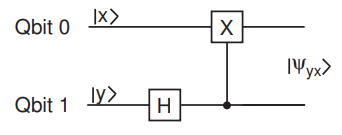
\includegraphics[scale=0.5]{entang}
\end{figure}



\noindent \textit{Solution:} $\mathbf{C}_{10}$ does nothing to Qbit 0 when Qbit 1 is in state 0, and flips Qbit 0 when Qbit 1 is in state 1. 
\begin{align}
\mathbf{C}_{10}\had_1 \ket{yx} &= \mathbf{C}_{10} (\had \otimes \Id) \ket{y}\ket{x}\nn\\
&= \mathbf{C}_{10} \lp \f{1}{\sqrt{2^1}}\lp \ket{0} + (-1)^y\ket{1} \rp \rp \otimes \ket{x}\nn\\
&= \f{1}{\sqrt{2}} \mathbf{C}_{10}\lp \ket{0x} + (-1)^y \ket{1 x} \rp\nn\\
&= \f{1}{\sqrt{2}} \lp \ket{0 x} + (-1)^y \ket{1\bar{x}} \rp\nn\\
&\equiv \ket{\psi_{yx}}
\end{align}\qed






           
\newpage












\noindent \textbf{3. Measurements of the Bell States.} The ``Bell States'' are the maximally entangled states

\begin{align}
\ket{\psi_{yx}} = \f{1}{\sqrt{2}}\lp \ket{0x} + (-1)^y\ket{1\bar{x}} \rp,
\end{align}
where $x,y \in \{0,1\}$. These are all orthogonal states. \\

\noindent If measurements are made in the computational basis, can you distinguish any one of these states from the others?\\




\noindent \textit{Solution:} We cannot uniquely determine which Bell state is being measured (in the computation basis) without ``untanglement'', i.e., reversing the process in the previous problem to get $\ket{yx}$ from $\ket{\psi_{yx}}$.\\

Suppose (to get a contradiction) that we can. Then consider this counter-example. When we measure Qbit 1 in either one of the four Bell states, we cannot distinguish the Bell states
\begin{align}
\ket{\psi_{00}} = \f{1}{\sqrt{2}}\lp \ket{00} + \ket{11} \rp\nn\\
\ket{\psi_{10}} = \f{1}{\sqrt{2}}\lp \ket{00} - \ket{11} \rp
\end{align}
from each other. In both cases, we find Qbit 1 to be in state 0 with probability 1/2. Also, in both cases, whenever Qbit 1 is in state 0, Qbit 0 is also in state 0. So, there is no way to distinguish these Bell states by measuring in the computational basis without transforming them first.\qed




\newpage















\noindent \textbf{4. Disentangling the Bell States.} Above you showed that the individual Bell states can all be created using a Hadamard gate on bit 0 and a cNOT gate using bit 0 as the control and bit 1 as the target. A question arises in quantum teleportation is ``which Bell state is the two-Qbit system in?'' Clearly you need to do something more than just make measurements to find out for sure which one it is. Design a system that will allow you to unambigouously identify which of the Bell states a two-Qbit system is in. To do this, you should consider figuring out a set of unitary operations that gives
\begin{align}
\ket{\psi_{yx}} \implies \ket{yx} \equiv \ket{y}\ket{x}
\end{align}
with $x,y \in \{0,1\}^2$, and demonstrate that it works for all four states.\\




\noindent \textit{Solution:} We use the fact that quantum computational transformations are reversible. From Problem 2, we know that $\ket{\psi_{yx}} = \mathbf{C}_{10}\had_1 \ket{yx}.$  By applying the inverse of $\mathbf{C}_{10}\had_1$ (whose existence is guaranteed) to $\ket{\psi_{yx}}$, we will get back $\ket{yx}$. We know that $\had^{-1} = \had$. Further, $(\mathbf{C}_{10})^{-1} = \mathbf{C}_{10}$ because
\begin{align}
\mathbf{C}_{10}\mathbf{C}_{10} \ket{yx} &= \mathbf{C}_{10}\ket{y}\ket{x\oplus y}\nn\\ 
&= \ket{y}\ket{x\oplus y \oplus y} \nn\\
&=\ket{yx} \nn\\
\iff \mathbf{C}_{10}\mathbf{C}_{10} &= \Id \iff \mathbf{C}_{10} = (\mathbf{C}_{10})^{-1}.
\end{align}
Therefore, 
\begin{align}
(\mathbf{C}_{10}\had_1)^{-1} &= \had_1^{-1}(\mathbf{C}_{10})^{-1} = \had_1 \mathbf{C}_{10}.
\end{align}
We will check that $\had_1 \mathbf{C}_{10}\ket{\psi_{yx}} = \ket{yx}$:
\begin{align}
\had_1 \mathbf{C}_{10}\ket{\psi_{yx}} &= \had_1 \mathbf{C}_{10}\lp \f{1}{\sqrt{2}}\lb \ket{0x} + (-1)^{y}\ket{1\bar{x}} \rb \rp\nn\\
&= \f{1}{\sqrt{2}} \had_1 \lp \ket{0x} + (-1)^y \ket{1x}  \rp\nn\\
&= \f{1}{\sqrt{2}} \lp \f{1}{\sqrt{2}}\lb \ket{0} + \ket{1}  \rb  + (-1)^y \f{1}{\sqrt{2}} \lb \ket{0} - \ket{1} \rb \rp \otimes \ket{x}\nn\\
&= \f{1}{2}\underbrace{\lp \ket{0} + \ket{1} + (-1)^{y}\ket{0} - (-1)^y\ket{1}  \rp}_{\boxed{?}} \otimes \ket{x}
\end{align}
To find $\boxed{?}$ we observe that
\begin{align}
\begin{cases}
\ket{0} + \ket{1} + (-1)^{y}\ket{0} - (-1)^y\ket{1} = 2\ket{0}, \quad \text{whenever } y = 0\\
\ket{0} + \ket{1} + (-1)^{y}\ket{0} - (-1)^y\ket{1} = 2\ket{1}, \quad \text{whenever }  y = 1
\end{cases}
\end{align}
and so $\boxed{?}$ is identically $2\ket{y}$. With this, 
\begin{align}
\had_1 \mathbf{C}_{10}\ket{\psi_{yx}} = \f{1}{2}\cdot 2\ket{y}\ket{x} \equiv \ket{yx}.
\end{align}\qed













\newpage

















\section{Problem set 5}










\noindent \textbf{1. Operator Communication.} This will get you to think about a problem related to ``superdense coding.'' Alice and Bob share a pair of Qbits in the entangled state $\ket{\psi_{01}}$. For
concreteness, assume that Alice possesses Qbit 0 and Bob possesses Qbit 1. Alice chooses to
apply one of four operators to her Qbit: $\Id, \X_0, \Y_0$, or $\Z_0$. After doing that she sends her
Qbit to Bob. Explain how Bob can unambiguously determine what one of the four operators
Alice applied to her one Qbit by operating on and making measurements of the Qbit pair
that he now possesses.\\




\noindent \textit{Solution:} 
Let Alice and Bob share a pair of Qbits in the entangled state $\ket{\psi_{01}}$:
\begin{align}
\ket{\psi_{01}}_{BA} = \f{1}{\sqrt{2}}\lp \ket{01}_{BA} + \ket{10}_{BA} \rp.
\end{align}
Alice can apply $\Id_0, \X_0, \Y_0,$ or $\Z_0$ on her one Qbit. In each case, the outcome is 
\begin{align}
&(\Id \otimes \Id)\ket{\psi_{01}} = \f{1}{\sqrt{2}}\lp \ket{01} + \ket{10} \rp = \ket{\psi_{01}}\nn\\
&(\Id \otimes \X)\ket{\psi_{01}} = \f{1}{\sqrt{2}}\lp \ket{00} + \ket{11} \rp = \ket{\psi_{00}}\nn\\
&(\Id \otimes \Y)\ket{\psi_{01}} = \f{1}{\sqrt{2}}\lp i(-1)^1\ket{00} + i(-1)^0\ket{11} \rp = \f{-i}{\sqrt{2}}\lp \ket{00}- \ket{11} \rp = -i\ket{\psi_{10}}\nn\\
&(\Id \otimes \Z)\ket{\psi_{01}} = \f{1}{\sqrt{2}}\lp (-1)^1\ket{01} + (-1)^0\ket{10} \rp = \f{-1}{\sqrt{2}}\lp \ket{01} - \ket{10} \rp = -\ket{\psi_{11}}.
\end{align}
What Bob can do given these (distinguishable) outputs is inverting them using $\had_1 \mathbf{C}_{10}$. By making measurements in the computational basis, Bob can determine exactly what operator Alice has used on her Qbit:
\begin{align}
\ket{\psi_{01}}  &\xrightarrow{\had_1\mathbf{C}_{10}} \ket{01} \implies \text{Alice used } \Id\nn\\
\ket{\psi_{00}}  &\xrightarrow{\had_1\mathbf{C}_{10}} \ket{00}\implies \text{Alice used } \X_0 \nn\\
-i\ket{\psi_{10}}  &\xrightarrow{\had_1\mathbf{C}_{10}} -i\ket{10}\implies \text{Alice used } \Y_0 \nn\\
-\ket{\psi_{11}}  &\xrightarrow{\had_1\mathbf{C}_{10}} -\ket{11}\implies \text{Alice used } \Z_0. 
\end{align}



\qed






















\newpage


\noindent \textbf{2. Partial Measurements.} Consider the entangled state
\begin{align}
\ket{\psi}_2 = \f{1}{\sqrt{2}}\ket{00} - \f{1}{{2}}\ket{10} + \f{i}{2}\ket{11}
\end{align}
Consider a partial measurement of the system where Qbit 1 is measured.
\begin{enumerate}[(a)]
	\item What is the probability that when Qbit 1 is measured the outcome will be a 0? What
	is the state of the system after that bit has been measured?

	\item What is the probability that when Qbit 1 is measured the outcome will be a 1? What
	is the state of the system after that bit has been measured?
\end{enumerate}








\noindent \textit{Solution:} 
\begin{enumerate}[(a)]
	\item The probability that when Qbit 1 is measured the outcome will be a 0 is $(1/\sqrt{2})^2 = \boxed{1/2}$. The state of the system after Qbit 1 has been measured to be 0 is 
	\begin{align}
	\ket{\psi'}_2 = \f{\f{1}{\sqrt{2}}\ket{00}  }{\norm{\f{1}{\sqrt{2}}\ket{00} }} = \boxed{\ket{00}}
	\end{align}
	\item  The probability that when Qbit 1 is measured the outcome will be a 1 is one minus the probability that when Qbit 1 is measured the outcome will be a 0. So, the answer is $1 - 1/2 = \boxed{1/2}$. The state of the system after Qbit 1 has been measured to be 1 is
	\begin{align}
	\ket{\psi'}_2 = \f{\f{-1}{2}\ket{00}+ \f{i}{2}\ket{11}   }{\norm{\f{-1}{2}\ket{00}+ \f{i}{2}\ket{11} }} = \boxed{\f{-1}{\sqrt{2}}\lp \ket{10} - i\ket{11} \rp}
	\end{align} 
\end{enumerate}\qed

























\newpage






















\noindent \textbf{3. Games with Algebra.} The original paper on quantum quantum teleportation by Bennett,
Brassard, Cr\'epeau, Jozsa, Peres, and Wooters in 1993 was described to me by Bill Wooters
as ``games with algebra.'' The original article can be found via this \href{https://pdfs.semanticscholar.org/a3e4/5ffd3886f1a26f849514de3791054eebcc42.pdf}{\underline{link}}.\\

\noindent Here's a way to understand the algebraic game. In the initial state of the system, Alice has
two Qbits (2 and 1) and Bob has one Qbit (0).  Qbits 1 and 0 are in the entangled state $\ket{\psi_{00}}$, and Qbit 2 is in an unknown state $\ket{\al} = \al_0 \ket{0} + \al_1 \ket{1}$.  The state is written most naturally
as a 3-bit partially entangled state
\begin{align}
\ket{\psi}_3 = \ket{\al}\ket{\psi_{00}}.
\end{align}
%or, expanding it out, we can write it as
%\begin{align}
%\ket{\psi}_3 = \f{1}{\sqrt{2}}\lp \al_0 \ket{000} + \al_0 \ket{011} + \al_1 \ket{100} + \al_1 \ket{111}  \rp.
%\end{align}
Show that this state can be written (most unnaturally!) as
\begin{align}
\ket{\psi}_3 = \f{1}{2} \lp \ket{\psi_{00}}\ket{\al} + \ket{\psi_{01}}\X\ket{\al} + \ket{\psi_{10}}\Z\ket{\al} + \ket{\psi_{11}}\X \Z \ket{\al} \rp
\end{align}
where the single-Qbit operators $\X$ and $\Z$ act only on Qbit 0 and the Bell-states are for Qbits 2 and 1. Explain how the observation that you just demonstrated provided the motivation for the
protocol that we discussed in class for quantum teleportation.\\




\noindent \textit{Solution:} 
We want to show that 
\begin{align}
\f{1}{2} \lp \ket{\psi_{00}}\ket{\al} + \ket{\psi_{01}}\X\ket{\al} + \ket{\psi_{10}}\Z\ket{\al} + \ket{\psi_{11}}\X \Z \ket{\al} \rp = \ket{\al}\ket{\phi_{00}},
\end{align}
to which end we use the identities:
\begin{align}
\X \ket{\al} &= \X (\al_0 \ket{0} + \al_1 \ket{1}) = \al_0\ket{1} + \al_1\ket{0}\nn\\
\Z \ket{\al} &= \Z (\al_0 \ket{0} + \al_1 \ket{1}) = \al_0 \ket{0} - \al_1\ket{1}\nn\\
\X\Z\ket{\al} &= \X (\al_0 \ket{0} - \al_1\ket{1}) = \al_0 \ket{1} - \al_1 \ket{0}.
\end{align}
We proceed by expanding the LHS until we get to the RHS:
\begin{align}
&\,\,\f{1}{2} \lp \ket{\psi_{00}}\ket{\al} + \ket{\psi_{01}}\X\ket{\al} + \ket{\psi_{10}}\Z\ket{\al} + \ket{\psi_{11}}\X \Z \ket{\al} \rp = \ket{\al}\ket{\phi_{00}}\nn\\
=&\,\, \f{1}{2\sqrt{2}}\lb \lp \ket{00} + \ket{11} \rp\lp \al_0 \ket{0} + \al_1 \ket{1} \rp  + \lp \ket{10} + \ket{01} \rp \lp \al_1\ket{0} + \al_0\ket{1} \rp\right.\nn\\
&\,\,\quad\left. + \lp \ket{00} - \ket{11} \rp  \lp \al_0 \ket{0} - \al_1\ket{1} \rp + \lp \ket{01} - \ket{10} \rp\lp \al_0\ket{1} - \al_1\ket{0} \rp  \rb\nn\\
=&\,\, \f{1}{2\sqrt{2}}\lb 2\al_0\ket{000} + (\al_1-\al_1) \ket{001} + (\al_1-\al_1)\ket{010} + 2\al_0 \ket{011} \right.\nn\\
&\,\,\quad\left. +2\al_1\ket{100} + (\al_0 - \al_0)\ket{101} + (\al_0 - \al_0)\ket{110} + 2\al_1 \ket{111} \rb\nn\\
=&\,\, \f{1}{\sqrt{2}} \lp \al_0 \ket{000} + \al_0 \ket{011} + \al_1\ket{100} + \al_1\ket{111} \rp\nn\\
=&\,\, (\al_0\ket{0} + \al_1\ket{1}) \f{1}{\sqrt{2}}\lp \ket{00} + \ket{11}  \rp\nn\\
=&\,\, \ket{\al}\ket{\psi_{00}}.
\end{align}

This result motivates the protocol for quantum teleportation in the following way. Suppose Alice (who is the sender in this case) has a Qbit in some arbitrary state $\ket{\al}$ and wants to send this state (not the Qbit, just the state) to Bob, without knowing what state his Qbit is in. What Alice and Bob can do is to have first share an pair of Qbits in the Bell state $\ket{00}$, each possessing one Qbit of the pair.  Then, they can consider the system of three Qbits whose state is $\ket{\psi}_3 = \ket{\al} \otimes \ket{\psi_{00}}$. From the exercise, we know that $\ket{\psi}_3$ can be written as
\begin{align}
\ket{\psi}_3 = \f{1}{2} \lp \ket{\psi_{00}}\ket{\al} + \ket{\psi_{01}}\X\ket{\al} + \ket{\psi_{10}}\Z\ket{\al} + \ket{\psi_{11}}\X \Z \ket{\al} \rp.
\end{align}
Now, we see that Alice's Qbits are in one of the four Bell states $\ket{\psi_{yx}}$. By applying the inversion $\had_2 \mathbf{C}_{21}$ to $\ket{\psi_{yx}}$, followed by measurements on the computational basis, Alice can send two classical bits $\ket{y}$ and $\ket{x}$, $x,y \in \{0,1\}$ to Bob. With these classical bits, there is a way for Bob to make sure his Qbit is in $\ket{\al}$:
\begin{itemize}
	\item If Alice sends $\ket{00}$,  Bob does nothing. His Qbit is already in $\ket{\al}$.
	\item If  Alice sends $\ket{01}$,  Bob applies $\X$ to his Qbit: $\X (\X \ket{\al}) = \ket{\al}$. 
	\item If Alice sends $\ket{10}$,  Bob applies $\Z$ to his Qbit: $\Z (\Z \ket{\al}) = \ket{\al}$.
	\item if Alice sends $\ket{11}$,  Bob applies $\Z\X$ to his Qbit: $\Z\X (\X\Z)\ket{\al} = \ket{\al}$.
\end{itemize}  
Here we rely on the fact that the Pauli matrices are involutory, i.e. $\sigma_i^2 = \Id, \forall i = 1,2,3$. \\

With this protocol, Alice can send the state $\ket{\al}$ of her Qbit to Bob's Qbit.  \qed
















\newpage
\noindent \textbf{4.} The goal of this problem is to consider a slightly simplified version of quantum teleportation. In this problem Alice and Bob start (as with most problems like this) by sharing two Qbits
in an entangled state. For the purposes of this problem the two QBits are an entangled pair of photons in the entangled (Bell) state
\begin{align}
\ket{\psi_{00}} = \f{1}{\sqrt{2}}\ket{00} + \f{1}{\sqrt{2}}\ket{11}.
\end{align}
Alice wants Bob to have a photon Qbit in a specific state $\ket{\phi}$ but wants to send Bob the
minimum amount of information possible for him to make it. The goal of this problem is to
show that (if they have the resource of an entangle Qbit pair) she can make that happen by
sending Bob only \textbf{one} classical bit of information.\\

\noindent Start by remembering the definition of a rotation operator $\mathbf{R}_\phi$ on photons, which takes a photon linearly polarized at angle $\al$ and converts it into a linearly polarized photon at angle
$\al + \phi$. The matrix representation of the rotation operator in the computational basis is
\begin{align}
\mathbf{R}_\phi = \begin{pmatrix}
\cos\phi & -\sin\phi \\ \sin\phi & \cos\phi
\end{pmatrix}.
\end{align}
As you showed on an earlier assignment $\mathbf{R}_\phi$ is a unitary operator with $\mathbf{R}_\phi^\dagger = \mathbf{R}^{-1}_\phi = \mathbf{R}_{-\phi}$ and $\mathbf{R}_\phi \ket{0} = \ket{\phi}$ and $\mathbf{R}_\phi \ket{1} = \ket{\pi/2 + \phi}$. To slightly simplify notation, call $\ket{\pi/2 + \phi} = \ket{\phi_\perp}$. 
\begin{enumerate}[(a)]
	\item Show that $ \Z \X\ket{\phi_\perp} = \ket{\phi}$.
	\item Show that the entangled (Bell) state $\ket{\psi_{00}}$ can also be written as 
	\begin{align}
	\ket{\psi_{00}} = \f{1}{\sqrt{2}}\ket{\phi\phi} + \f{1}{\sqrt{2}}\ket{\phi_\perp \phi_\perp}.
	\end{align}
	This says something special about the state $\ket{\psi_{00}}$. What? 
	\item Imagine that Alice applies the operator $\mathbf{R}_\phi^{-1}$ to her Qbit. What is the state of the system after she does that?
	\item Alice measures her QBit. What is the probability that she measures 0? What is the
	probability that she measures 1?
	\item What state does Bob’s QBit have if Alice measures 0? What state does Bob’s QBit have
	if she measures 1?
	\item If Alice tells Bob the value that she measured, what can he do to assure himself that his
	Qbit is in the state $\ket{\phi}$? 
\end{enumerate}



\newpage
\noindent \textit{Solution:} 
\begin{enumerate}[(a)]
	\item We want to show that $\Z\X \mathbf{R}_{\pi/2} = \Id$, since 
	\begin{align}
	\Z\X\ket{\phi_\perp} = \ket{\phi} \forall \ket{\phi} &\iff \Z \X \mathbf{R}_{\pi/2}\ket{\phi} = \ket{\phi} \forall \ket{\phi}\nn\\
	&\iff \Z \X \mathbf{R}_{\pi/2} \equiv \Id.
	\end{align}
	Since $\Z \X \mathbf{R}_{\pi/2}$ is a linear operator, its action is completely determined by what it does to the basis vectors:
	\begin{align}
	&\Z \X \mathbf{R}_{\pi/2}\ket{0} = \Z \X \ket{\pi/2} = \Z \ket{0} = \ket{0}\nn\\
	&\Z \X \mathbf{R}_{\pi/2}\ket{1} = \Z \X \ket{\pi} = -\Z \X \ket{0} = -\Z\ket{1} = \ket{1},
	\end{align}
	where we have used the fact that $\ket{1} \equiv \ket{\pi/2}$ and $-\ket{0} \equiv \ket{\pi}$. This can readily be checked by plugging in values of $\phi$ into $\begin{pmatrix}
	\cos \phi & \sin\phi
	\end{pmatrix}^\top$. \\
	
	Since $\Z \X \mathbf{R}_{\pi/2}$ acts as the identity function on the entire computational basis, it \textit{is} the identity function, by linearity. Evidently: for any $\ket{\phi} = \cos\phi \ket{0} + \sin\phi \ket{1}$, 
	\begin{align}
	\Z \X \mathbf{R}_{\pi/2}(\cos\phi \ket{0} + \sin\phi \ket{1}) = \cos\phi \ket{0} + \sin\phi \ket{1} \equiv \ket{\phi}.
	\end{align}
	
	
	
	Therefore,
	\begin{align}
	\ket{\phi} = \Z \X \mathbf{R}_{\pi/2}\ket{\phi} = \Z \X \ket{\phi_\perp}, \forall \ket{\phi}.
	\end{align}
	
	
	\item In the computational basis, $\ket{\phi} = \begin{pmatrix}
	\cos\phi & \sin\phi
	\end{pmatrix}^\top$, and $\ket{\phi_\perp} = \begin{pmatrix}
	-\sin\phi & \cos\phi
	\end{pmatrix}^\top$. With these, we expand the RHS to (hopefully) get the LHS: 
	\begin{align}
	&\f{1}{\sqrt{2}}\lp \ket{\phi\phi} + \ket{\phi_\perp\phi_\perp} \rp\nn\\
	=& \f{1}{\sqrt{2}}\lb \begin{pmatrix}
	\cos\phi \\ \sin\phi
	\end{pmatrix} \otimes \begin{pmatrix}
	\cos\phi \\ \sin\phi
	\end{pmatrix} + \begin{pmatrix}
	-\sin\phi \\ \cos\phi
	\end{pmatrix} \otimes \begin{pmatrix}
	-\sin\phi \\ \cos\phi
	\end{pmatrix} \rb\nn\\
	=& \f{1}{\sqrt{2}}\lb \begin{pmatrix}
	\cos^2\phi \\ \f{\sin 2 \phi}{2} \\ \f{\sin 2\phi}{2} \\ \sin^2\phi \\ 
	\end{pmatrix} + \begin{pmatrix}
	\sin^2\phi \\ -\f{\sin 2 \phi}{2} \\ -\f{\sin 2 \phi}{2} \\ \cos^2\phi
	\end{pmatrix} \rb\nn\\
	=& \f{1}{\sqrt{2}}\begin{pmatrix}
	1 & 0 & 0 & 1
	\end{pmatrix}^\top\nn\\
	\equiv& \ket{\phi_{00}}.
	\end{align}
	So we're done. This result says that $\ket{\phi_{00}}$ is invariant under rotations by $\phi$ on both Qbits, i.e. $\mathbf{R}_\phi\otimes\mathbf{R}_\phi\ket{\psi_{00}}= \ket{\psi_{00}}$. Further, by the previous part, $\ket{\psi_{00}}$ is also invariant under $(\Z\X)\otimes (\Z\X)$, by symmetry:
	\begin{align}
	(\Z \X) \otimes (\Z\X)\ket{\psi_{00}} \xrightarrow{\phi \leftrightarrow \phi_\perp} \ket{\psi_{00}}.
	\end{align}
	
	\item Let 
	\begin{align}
	\ket{\phi_{00}} = \f{1}{\sqrt{2}}\lp \ket{\phi\phi}  + \ket{\phi_\perp\phi_\perp}\rp
	\end{align}
	be given. By the previous part, we know that the expression above is equivalent to $(1/\sqrt{2})\lp \ket{00} + \ket{11} \rp$. So, when Alice applies the operator $\mathbf{R}_{\phi}^{-1} \equiv \mathbf{R}_{-\phi}$ to her (0) Qbit, $\ket{\phi_{00}}$ is transformed into
	\begin{align}
	(\Id \otimes \mathbf{R}_{-\phi})\ket{\psi_{00}} &= \f{1}{\sqrt{2}}\lp \ket{\phi}\mathbf{R}_{-\phi}\ket{\phi} + \ket{\phi_\perp}\mathbf{R}_{-\phi}\ket{\phi_\perp} \rp\nn\\
	&= \boxed{\f{1}{\sqrt{2}}\lp \ket{\phi 0} + \ket{\phi_\perp 1} \rp}
	\end{align}
	where we have used the identifications: $\ket{\phi_\perp} \equiv\ket{\phi + \pi/2}$ and $\ket{\pi/2} \equiv \ket{1}$. 
	
	
	\item Evidently, the probability that Alice measures 0 is 1/2, because $(\Id \otimes \mathbf{R}_{-\phi})\ket{\psi_{00}}$ is in equal superposition of $\ket{\phi 0}$ and $\ket{\phi_\perp 1}$. By symmetry, the probability that Alice measures 1 is also 1/2 
	
	\item  If Alice measures 0, then Bob's Qbit is in the state $\ket{\phi}$. If Alice measures 1, then Bob's Qbit is in the state $\ket{\phi_\perp}$.
	
	
	\item Let Alice's measurement be given as $x \in \{0,1\}$. To ensure that his Qbit is in the state $\ket{\phi}$, Bob must leave his Qbit (in state $\ket{\phi}$) alone if $x=0$ and apply $\Z\X$ to his Qbit (now in state $\ket{\phi_\perp}$) to change it to $\ket{\phi}$ if $x = 1$. \\
	
	The protocol can be summarized as
	\begin{align}
	\begin{cases}
	x = 0 \implies \text{Bob does nothing to his Qbit} \implies \Id\ket{\phi} = \ket{\phi}\\
	x = 1 \implies \text{Bob applies $\Z\X$ to his Qbit} \implies \Z \X \ket{\phi_\perp} = \ket{\phi}.
	\end{cases}
	\end{align}
	
	We can write this protocol more concisely as $\boxed{\lp \Z \X \rp^x, x \in \{0,1\}}$. 
	

	
	
	
\end{enumerate}\qed























\newpage





\section{Problem set 6}



\noindent \textbf{1. Monroe Colloquium}\\



\noindent \textbf{2. Deutsch's Original Algorithm.} In class on March 12th we discussed the Deutsch problem. Determining if a function $f(x)$ is either constant or balanced, where $x$ is a single bit.\\

\noindent There are four functions on one bit, $f_0$ gives the constant output $0$, $f_1$ gives the constant output $1$, $f_b$ (buffer) gives an output equal to the input, and $f_i$ (invert) has an output
equal to ¯$x$. The functions $f_0$ and $f_1$ are constant, and the functions $f_b$ and $f_i$ are balanced.
Tabulated they are:\\
\begin{center}
\begin{tabular}{|c|c|c|}
	\hline
	$x$&0&1\\
	\hline
	$f_0(x)$&0&0\\
	\hline
	$f_1(x)$&1&1\\
	\hline
	$f_b(x)$&0&1\\
	\hline
	$f_i(x)$&1&0\\
	\hline
\end{tabular}
\end{center}

\noindent In Appendix F, Mermin looks at the approach that Deutsch originally considered (in 1985) for determining if a function $f : \{0, 1\} \to \{0, 1\}$ is balanced or constant. As mentioned in class the algorithm outlined in Mermin Chapter 2 and in class was developed much later (1997) by Cleve, Ekert, Macchiavello, and Mosca using the idea of ``phase kickback.''\\

\noindent Consider the ``quantum parallelism'' approach to the Deutsch problem shown below as a quantum circuit diagram.
\begin{figure}[!htb]
	\centering
	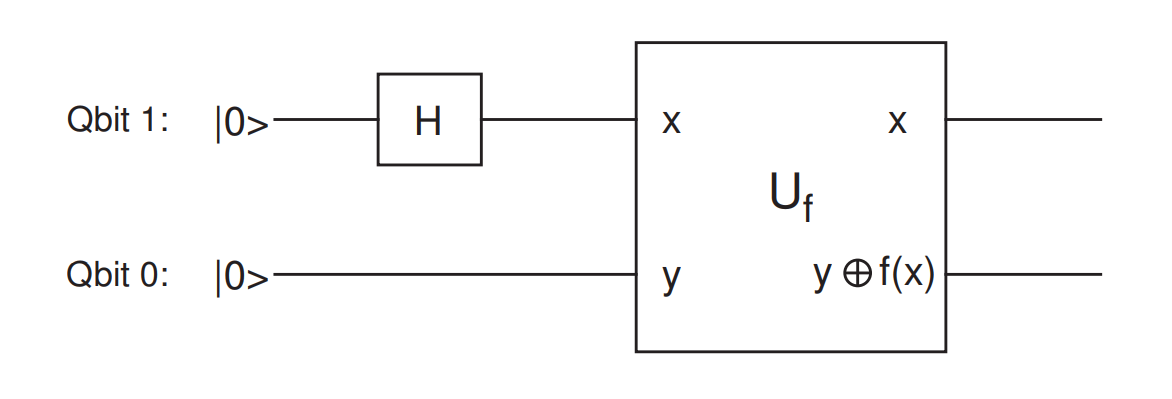
\includegraphics[scale=0.25]{deutsch}
\end{figure}

\noindent In the diagram Qbit 1 is the ``input register'' and Qbit 0 is the ``output register.''

\begin{enumerate}[(a)]
	\item Show that the output of the operator $\mathbf{U}_f$ is, as written in Eq. F.2-F.5 in Mermin
	\begin{align*}
	\ket{\psi_0} &= \ket{+}\ket{0}\nn\\
	\ket{\psi_1} &= \ket{+}\ket{1}\nn\\
	\ket{\psi_b} &= \f{1}{\sqrt{2}}\lp \ket{0}\ket{0} + \ket{1}\ket{1} \rp = \ket{\psi_{00}}\nn\\
	\ket{\psi_i} &= \f{1}{\sqrt{2}}\lp \ket{0}\ket{1} + \ket{1}\ket{0} \rp = \ket{\psi_{01}}
	\end{align*}
	The states due to the constant functions are product states, and the output states due to the balanced functions are two of the entangled Bell states. Deutsch’s idea was to show that you could manipulate the output state in such a way that a measurement of the output could distinguish between constant and balanced functions half the time, but that half the time you would make a measurement that gave no information at all.
	
	\item Think about measuring the states of Qbits 0 and 1 for the four different states above. What does it allow you to distinguish about the states?
	
	
	\item Consider the approach described by Mermin when you apply a Hadamard gate to both Qbits 0 and 1 after the application of $\mathbf{U}_f$. Show that Eqs. F.6-F.9 in Mermin are correct, namely that
	\begin{align}
	\had^{\otimes 2}\ket{\psi_0} &= \f{1}{\sqrt{2}}\lp \ket{00} + \ket{01} \rp\nn\\
	\had^{\otimes 2}\ket{\psi_1} &= \f{1}{\sqrt{2}}\lp \ket{00} - \ket{01} \rp\nn\\
	\had^{\otimes 2}\ket{\psi_b} &= \f{1}{\sqrt{2}}\lp \ket{00} + \ket{11} \rp = \ket{\psi_{00}}\nn\\
	\had^{\otimes 2}\ket{\psi_i} &= \f{1}{\sqrt{2}}\lp \ket{00} - \ket{11} = \ket{\psi_{10}} \rp
	\end{align}
	where $\had^{\otimes 2}$ is the Hadamard gate applied to both Qbits. 
	
	
	\item In your own words, explain how these states allow you to determine whether or not the
	function is constant or balance half the time.
	
	
	\item (Optional. For those who took PH431.) Follow, and outline in detail, Mermin’s argument
	that there is NO possible operation you can do to the two output Qbits that allow you
	to determine whether the function is balanced or constant with certainty (100\% of the
	time).
	
	
	\item (Optional$^2$. For those who are looking for a serious challenge.) Follow, and outline in
	detail, Mermin’s argument that the best you can do with operations on the two output
	Qbits is to determine whether the function is balanced or constant 50\% of the time.
	
	
	
	
	
	
	
	
	
	
\end{enumerate}



\noindent \textit{Solution:} 
\begin{enumerate}[(a)]
	\item The unitary $\mathbf{U}_f$ is such that
	\begin{align}
	\mathbf{U}_f \ket{xy} = \ket{x}\ket{y\oplus f(x)},
	\end{align}
	where $y\in \{0,1\}$ and $\ket{x} = \had\ket{x'} = \ket{\pm}$ with $x' \in \{0,1\}$. With this, the general output of $\mathbf{U}_f$ has the form:
	\begin{align}
	\mathbf{U}_f\lp \had_1\ket{00} \rp 
	&= \f{1}{\sqrt{2}}\mathbf{U}_f(\ket{00}+\ket{10})\nn\\
	&= \f{1}{\sqrt{2}}\lp \ket{0}\ket{0\oplus f(0)} + \ket{1}\ket{0\oplus f(1)} \rp\nn\\
	&= \frac{1}{\sqrt{2}}\lp \ket{0}\ket{f(0)} + \ket{1}\ket{f(1)} \rp
	\end{align}
	like that in Eq. F-1. It follows that the four possible $f$'s and associated outputs of $\mathbf{U}_f$ are
	\begin{align}
	&f \equiv f_0: \quad \ket{\psi_0} = \mathbf{U}_f\lp \had_1\ket{00} \rp 
	= \f{1}{\sqrt{2}}\lp \ket{0}\ket{0} + \ket{1}\ket{0} \rp 
	= \ket{+}\ket{0} \nn\\
	&f \equiv f_1: \quad \ket{\psi_1} = \mathbf{U}_f\lp \had_1\ket{00} \rp 
	= \f{1}{\sqrt{2}}\lp \ket{0}\ket{1} + \ket{1}\ket{1} \rp 
	= \ket{+}\ket{1} \nn\\
	&f \equiv f_b: \quad \ket{\psi_b} = \mathbf{U}_f\lp \had_1\ket{00} \rp 
	=  \f{1}{\sqrt{2}}\lp \ket{0}\ket{0} + \ket{1}\ket{1} \rp\nn\\
	&f \equiv f_i: \quad \ket{\psi_i} = \mathbf{U}_f\lp \had_1\ket{00}\rp 
	=  \f{1}{\sqrt{2}}\lp \ket{0}\ket{1} + \ket{1}\ket{0} \rp.
	\end{align}
	where the values of $f$ for each $f_j$ is tabulated above. 
	
	
	\item Looking at the general form of $\mathbf{U}_f$ again,
	\begin{align}
	\ket{\psi} = \f{1}{\sqrt{2}}\lp \ket{0}\ket{f(0)} + \ket{1}\ket{f(1)} \rp,
	\end{align}
	we see that a direct measurement of both Qbits reveals the value $f$ takes at either $0$ or $1$. In particular, suppose we see Qbit 0 in state 0. Then, if we see Qbit 1 in state 0 then we know $f$ is either $f_0$ or $f_b$ but can't tell which is $f$ is; similarly, if we see Qbit 1 in state 1 then we know $f$ is either $f_0$ or $f_i$ but can't tell which is $f$. Repeating this argument for state 1, we see that we cannot distinguish $f_1$ from $f_i$ and $f_1$ from $f_b$. To resolve this problem, we will want to distinguish between the two cases:
	\begin{align}
	\mbox{\textbf{Case 1:}}\quad \ket{\psi} = \ket{\psi_0} \mbox{or} \ket{\psi_1};\quad 	\mbox{\textbf{Case 2:}}\quad \ket{\psi} = \ket{\psi_i} \mbox{or} \ket{\psi_b}
	\end{align} 
	To this end, we will want to use a $\had^{\otimes 2}$ that appears in the next item. 
		
	
	
	
	
	\item In this item, we are just verifying that $\had^{\otimes 2}$ transforms the outputs in part (a) into those given in part (c):
	\begin{align}
	\had^{\otimes 2}\ket{\psi_0} &= \had^{\otimes 2} \lp \ket{+}\ket{0}\rp\nn\\
	&= \had\ket{+} \otimes \had\ket{0}\nn\\
	&= \ket{0} \otimes \ket{+}\nn\\
	&= \f{1}{\sqrt{2}}   \lp \ket{00} + \ket{01}  \rp
	\end{align}
	\begin{align}
	\had^{\otimes 2}\ket{\psi_1} &= \had^{\otimes 2} \lp \ket{+}\ket{1}\rp \nn\\
	&= \had\ket{+}\otimes \had\ket{1}\nn\\
	&= \ket{0}\otimes \ket{-}\nn\\
	&= \f{1}{\sqrt{2}} \lp \ket{00} - \ket{01}  \rp
	\end{align}
	\begin{align}
	\had^{\otimes 2}\ket{\psi_b} &= \had^{\otimes 2} \lp \f{1}{\sqrt{2}}\lp \ket{0}\ket{0} + \ket{1}\ket{1} \rp\rp\nn\\
	&= \f{1}{\sqrt{2}}\lp \ket{+}\ket{+} + \ket{-}\ket{-} \rp\nn\\
	&= \f{2}{2\sqrt{2}}\lp \ket{00} + \ket{11} \rp\nn\\
	&= \f{1}{\sqrt{2}}\lp \ket{00} + \ket{11} \rp
	\end{align}
	\begin{align}
	\had^{\otimes 2}\ket{\psi_i} &= \had^{\otimes 2} \lp \f{1}{\sqrt{2}}\lp \ket{0}\ket{1} + \ket{1}\ket{0} \rp\rp\nn\\
	&= \f{1}{\sqrt{2}}\lp \ket{+}\ket{-} + \ket{-}\ket{+} \rp\nn\\
	&= \f{2}{2\sqrt{2}}\lp \ket{00} - \ket{11}   \rp \nn\\
	&= \f{1}{\sqrt{2}}\lp \ket{00} - \ket{11} \rp.
	\end{align}
	
	
	\item Suppose we measure both Qbits. If $f$ is a constant function, then we will see $00$ half the time and $01$ half the time. If $f$ is balanced, then we will see $00$ half the time and $11$ half the time. So, for any $f$, we will always see $00$ half the time. In the other half of the time we will see either $11$ or $01$, from which we can deduce (with absolute certainty) either $f$ is balanced (if $11$) or constant (if $01$). So, the probability of success here is $50\% \times 100\% = 50\%$. 
	
	
	
	\item \underline{Claim}: There is no transformation on $\ket{\psi} =  \mathbf{U}_f\had_1\ket{00}$ that could enable one to tell whether $f$ is constant or balanced with certainty. 
	
	\begin{proof}
		Suppose (to get a contradiction) that there exists such a (unitary) 2-Qbit transformation. We will call it $\mathbf{U}$. For $\mathbf{U}$ to work, it must be such that each measurement on a Qbit is ``meaningful.'' In particular, $\mathbf{U}$ should not act like $\had$ which allows $\ket{00}$ to appear in all of the outputs, rendering the observation $00$ meaningless. This imposes the condition that the computational basis states that appear in $\mathbf{U}\ket{\psi_0}$ and $\mathbf{U}\ket{\psi_1}$ cannot appear in $\mathbf{U}\ket{\psi_b}$ and $\mathbf{U}\ket{\psi_i}$ (and vice versa), because otherwise this ``common basis state, $\ket{e}$'' will appear as $\mathbf{U}\ket{e}$ output states of both cases of $f$, making the probability of successfully discriminating the cases less than 1. We claim, however, that this condition cannot be satisfied for the following reason: The condition above implies that the vector space spanned by the computation basis can be decomposed into a direct sum of orthogonal subspaces $\V \oplus \V^\perp$, where $\mathbf{U}\ket{\psi_0}, \mathbf{U}\ket{\psi_1} \in \V$, and $\mathbf{U}\ket{\psi_i}, \mathbf{U}\ket{\psi_b}\in \V^\perp$. It follows that $v\perp v'\,\forall v\in \V, v'\in \V^\perp$. In particular, we must have that
		\begin{align}
		0=\braket{\mathbf{U}\psi_{1,0}}{\mathbf{U}\psi_{i,b}} = \braket{\mathbf{U}^\dagger\mathbf{U}\psi_{1,0}}{\psi_{i,b}} = \braket{\psi_{1,0}}{\psi_{i,b}}
		\end{align}  
		when in fact
		\begin{align}
		\braket{\psi_{1,0}}{\psi_{i,b}} = 1/2.
		\end{align}
		So that's a contradiction. Thus, no such $\mathbf{U}$ exists.
	\end{proof}
	
	
	
	
	\item \underline{Claim:} The probability of correctly determining whether $f$ is constant or balanced (by applying a unitary to $\mathbf{U}_f\had_1\ket{00}$) is \textit{at most} 50\%.
	\begin{proof}
		Suppose we bring in $n$ additional ancillary Qbits. These might be used to transform the input and output registers after the application of $\mathbf{U}_f$ on the Qbits 0 and 1. Let a unitary $\mathbf{W}$ denote this transformation. $\mathbf{W}$ acts on the state space spanned by $n+2$ Qbits. Suppose further (without loss of generality) that these $n$ Qbits are initially in $\ket{0}_n$ (since any general state $\ket{\chi}_n$ can be written as $\mathbf{\mathcal{U}}\ket{0}_n$ where $\mathcal{U}$ is some unitary, which we let $\mathbf{W}$ absorb). \\
		
		Now let the state $\ket{\psi} = \mathbf{U}_f\had_1\ket{00}$ be given. Let $\mathbf{W}$ act on $\ket{\psi}$. The probability of measuring $x_2\in [0,2^2)$ for the Qbit pair and $y_n\in [0,2^n)$ for the $n$ additional Qbits is given by
		\begin{align}
		{\Pr}_{\ket{\psi}_2}(x_2,y_{n}) = \abs{ \bra{x_2y_n} \mathbf{W}\ket{\psi_2,0_n}}^2 = 0
		\end{align}
		where the short-hand $\ket{\psi_2,0_n}$ denotes $\ket{\psi}_2\otimes \ket{0}_n$. Let any arbitrary pair state $\ket{\phi}$ given, then
		\begin{align}
		{\Pr}_{\ket{\phi}_2}(x,y)= 0 \iff \bra{x_2y_n} \mathbf{W}\ket{\phi_2,0_n} = 0.
		\end{align}
		Suppose these $\ket{\phi}$'s span some subspace $\V$ and that ${\Pr}_{\ket{\phi}} (x,y) = 0$ for all $\ket{\phi}$, then linearity says that for any $v \in \V$, ${\Pr}_v(x,y) = 0$ as well. Now, consider (again) the four possible states of $\mathbf{U}_f\had_1\ket{00}$:
		\begin{align}
		&f \equiv f_0: \quad \ket{\psi_0} = \mathbf{U}_f\lp \had_1\ket{00} \rp 
		= \f{1}{\sqrt{2}}\lp \ket{0}\ket{0} + \ket{1}\ket{0} \rp 
		= \ket{+}\ket{0} \nn\\
		&f \equiv f_1: \quad \ket{\psi_1} = \mathbf{U}_f\lp \had_1\ket{00} \rp 
		= \f{1}{\sqrt{2}}\lp \ket{0}\ket{1} + \ket{1}\ket{1} \rp 
		= \ket{+}\ket{1} \nn\\
		&f \equiv f_b: \quad \ket{\psi_b} = \mathbf{U}_f\lp \had_1\ket{00} \rp 
		=  \f{1}{\sqrt{2}}\lp \ket{0}\ket{0} + \ket{1}\ket{1} \rp\nn\\
		&f \equiv f_i: \quad \ket{\psi_i} = \mathbf{U}_f\lp \had_1\ket{00}\rp 
		=  \f{1}{\sqrt{2}}\lp \ket{0}\ket{1} + \ket{1}\ket{0} \rp.
		\end{align}
		Any measurement that allows us to distinguish with certainty \textbf{Case 1} from \textbf{Case 2} must have \textit{zero} probability for detecting either (i) any linear combination of $\ket{\psi_0}$ and $\ket{\psi_1}$ OR (ii) any linear combination of $\ket{\psi_i}$ and $\ket{\psi_b}$ (this OR is exclusive). Otherwise, if there's some nonzero probability of detecting some states in both \textbf{Case 1} and \textbf{Case 2} then we cannot distinguish the cases. \\
		
		With this, we consider the state
		\begin{align}
		\ket{\al} = \f{1}{2}\lp \ket{00} + \ket{01} + \ket{10} + \ket{11}  \rp.
		\end{align}
		We notice that $\ket{\al}$ requires the full 2-Qbit computational basis to describe. Any measurement outcomes $x,y$ with $ {\Pr}_{\ket{\al}} (x,y) \neq 0$ is meaningless. It follows that the probability of a measurement outcome that \textit{fails} to discriminate \textbf{Case 1} from \textbf{Case 2} is \textit{at least}:
		\begin{align}
		{\Pr}_{\mbox{min}} = \sum\limits_{\substack{x,y\\{\Pr}_{\ket{\al}} (x,y) \neq 0}} {\Pr}_{\ket{\psi}} (x,y).
		\end{align}
		Next, we want to relate $\ket{\psi}$ to $\ket{\al}$. It turns out that every one of $\ket{\psi}$ can be written as
		\begin{align}
		\ket{\psi} = \f{1}{\sqrt{2}}\lp \ket{\al} + \ket{\be} \rp
		\end{align}
		where $\ket{\be} \perp \ket{\al}$. Explicitly:
		\begin{align}
		\ket{\psi_0} = \f{1}{\sqrt{2}}\lb \ket{\al} + \f{1}{2}\lp \ket{00} - \ket{01} + \ket{10} - \ket{11}  \rp   \rb\nn\\
		\ket{\psi_1} = \f{1}{\sqrt{2}}\lb \ket{\al} - \f{1}{2}\lp \ket{00} - \ket{01} + \ket{10} - \ket{11}  \rp  \rb\nn\\
		\ket{\psi_b} = \f{1}{\sqrt{2}}\lb \ket{\al} + \f{1}{2}\lp \ket{00} - \ket{01} - \ket{10} + \ket{11}  \rp   \rb\nn\\
		\ket{\psi_i} = \f{1}{\sqrt{2}}\lb \ket{\al} - \f{1}{2}\lp \ket{00} - \ket{01} - \ket{10} + \ket{11}  \rp    \rb
		\end{align}
		From here, we have that
		\begin{align}
		{\Pr}_{\ket{\psi}} (x,y) &= \abs{\bra{x,y} \mathbf{W}\ket{\psi,0}}^2 \nn\\
		&= \f{1}{2}\abs{\bra{x,y} \mathbf{W}\ket{\al,0} + \bra{x,y} \mathbf{W}\ket{\be,0}}^2\nn\\
		&= \f{1}{2}\lp {\Pr}_{\ket{\al}}(x,y) + {\Pr}_{\ket{\be}}(x,y) + 2\Re\lc \bra{\be,0}\mathbf{W}^\dagger\ket{x,y}\bra{x,y}\mathbf{W}\ket{\al,0}  \rc  \rp
		\end{align}
		where we have used the identity
		\begin{align}
		\abs{a+b}^2 &= (a+b)\cdot(\overline{a+b})\nn\\
		&= \abs{a}^2 + \abs{b}^2 + \underbrace{a\bar{b} + \bar{a}b}\nn\\
		& = \abs{a}^2 + \abs{b}^2 + 2\Re{a\cdot \bar{b}}.
		\end{align}
		And so we have
		\begin{align}
		{\Pr}_{\mbox{min}} &= \sum\limits_{\substack{x,y\\{\Pr}_{\ket{\al}} (x,y) \neq 0}} {\Pr}_{\ket{\psi}} (x,y)\nn\\
		&= \f{1}{2}\sum\limits_{\substack{x,y\\{\Pr}_{\ket{\al}} (x,y) \neq 0}}\lb  {\Pr}_{\ket{\al}}(x,y) + {\Pr}_{\ket{\be}}(x,y)\right.\nn\\
		&\qquad\left. + 2\Re\lc \bra{\be,0}\mathbf{W}^\dagger\ket{x,y}\bra{x,y}\mathbf{W}\ket{\al,0}  \rc   \rb
		\end{align}
		Now, we will extend this sum to all $x,y$. We notice that
		\begin{align}
		\sum_{x,y}{\Pr}_{\ket{\al}}(x,y) &= \underbrace{\sum\limits_{\substack{x,y\\{\Pr}_{\ket{\al}} (x,y) \neq 0}} {\Pr}_{\ket{\al}}(x,y)}_{1} + \underbrace{\sum\limits_{\substack{x,y\\{\Pr}_{\ket{\al}} (x,y) = 0}} {\Pr}_{\ket{\al}}(x,y)}_{0}\nn\\
		&=1,
		\end{align}
		and 
		\begin{align}
		2\Re \sum_{x,y}  \bra{\be,0}\mathbf{W}^\dagger\ket{x,y}\bra{x,y}\mathbf{W}\ket{\al,0}   &=  2\Re \bra{\be,0} \mathbf{W}^\dagger\mathbf{W}\ket{\al,0}\nn\\
		&= 2\Re\bra{\be,0}\Id\ket{\al,0}\nn\\
		&= 2\Re\braket{\be,0}{\al,0}\nn\\
		&= 0,
		\end{align}
		where we have used the completion property and that $\ket{\al}$ and $\ket{\be}$ are orthogonal. So,
		\begin{align}
		{\Pr}_{\mbox{min}} = \f{1}{2}\lp 1 +  \sum\limits_{\substack{x,y\\{\Pr}_{\ket{\al}} (x,y) \neq 0}} {\Pr}_{\ket{\be}}(x,y) \rp \geq \f{1}{2}. 
		\end{align}
		So, the probability of failing is at least $1/2$, i.e. the probability of success is at most $1/2$. 
		
		
	\end{proof} 
	
	
	
	
	
	
	
	
\end{enumerate}





\newpage



\noindent \textbf{3. The binary dot product.} In several problems we’ll see during the rest of the semester we
will see the ``dot product'' $a \cdot b$ appear. This represents the ``bitwise'' inner product of two $n$-bit binary numbers $a$ and $b$
\begin{align}
a\cdot b \equiv_2 a_{n-1}b_{n-1} + \dots + a_1b_1 + a_0b_0 .
\end{align}
In quantum computer science the dot product is defined modulo-2, which means that it is given by a one-bit number - zero if the dot product is even, and 1 if the dot product is odd.
\begin{enumerate}[(a)]
	\item For two five bit numbers $a = 10101$ and $b = 11011$, what is the dot product $a \cdot b$? How about for $a = 11001$ and $b = 11011$?
	
	\item Show that the ``normal'' way (not modulo 2) of calculating the dot product gives the same result for
	\begin{align}
	\phi = (-1)^{a\cdot b}.
	\end{align}
	Most of the time we use it, the dot product will appear in this form.
	
	
	\item Show that the dot product could also be written
	\begin{align}
	a\cdot b = a_{n-1}b_{n-1} \oplus\dots \oplus a_1b_1 \oplus a_0b_0
	\end{align}
	which is how Mermin writes it.
\end{enumerate}








\noindent \textit{Solution:}


\begin{enumerate}[(a)]
	\item We just apply the formula given in the problem to compute these values:
	\begin{align}
	&10101 \cdot 11011 \equiv_2 1\cdot 1 + 0\cdot 1 + 1\cdot 0 + 0 \cdot 1 + 1 \cdot 1 \equiv_2 1 + 1 \equiv_2 \boxed{0}\nn\\
	&11001 \cdot 11011 \equiv_2 1\cdot 1 + 1 \cdot 1 + 0 \cdot 0 + 0 \cdot 1 + 1\cdot 1 \equiv_2 1 + 1 + 1\equiv_2 \boxed{1}\nn
	\end{align} 
	\item Let  $c = a\cdot b$ (without modulo 2). We know that $c \text{ odd } \iff c\text{ mod } 2 = 1$. So, $(-1)^c = (-1)^{c\text{ mod } 2}$ for all values of $c = a\cdot b$.  

	\item The addition $\oplus$ is addition mod 2. \underline{To prove}:
	\begin{align}
	a\cdot b = a_{n-1}b_{n-1} \oplus\dots \oplus a_1b_1 \oplus a_0b_0 \equiv_2 a_{n-1}b_{n-1} + \dots + a_1b_1 + a_0b_0
	\end{align}
	We can do this by induction. Suppose $n=1$, then $a,b\in \{0,1\}$. Because $a,b\in \{0,1\}$, $a\cdot b \equiv_2 ab$. So this base case holds. Next, suppose the statement holds up to $n$, i.e.,
	\begin{align}
	a_{n-1}b_{n-1} \oplus\dots \oplus a_1b_1 \oplus a_0b_0 \equiv_2 a_{n-1}b_{n-1} + \dots + a_1b_1 + a_0b_0.
	\end{align}  
	We want to show it also holds for $n+1$:
	\begin{align}
	a_{n}b_{n} \oplus\dots \oplus a_1b_1 \oplus a_0b_0 \equiv_2 a_{n}b_{n} + \dots + a_1b_1 + a_0b_0.
	\end{align} 
	We write the RHS as
	\begin{align}
	&a_nb_n + \lp a_{n-1}b_{n-1} + \dots + a_1b_1 + a_0b_0 \rp \nn\\
	\equiv_2\,\,& a_nb_n + \lp a_{n-1}b_{n-1} \oplus\dots \oplus a_1b_1 \oplus a_0b_0 \rp.
	\end{align}
	We notice that $a_n,b_n\in \{0,1\}$ and $a_{n-1}b_{n-1} \oplus\dots \oplus a_1b_1 \oplus a_0b_0 \in \{0,1\}$. By the definition of $\oplus$, we have
	\begin{align}
	&a_nb_n + \lp a_{n-1}b_{n-1} \oplus\dots \oplus a_1b_1 \oplus a_0b_0 \rp\nn\\ 
	\equiv_2\,\,& a_nb_n \oplus \lp a_{n-1}b_{n-1} \oplus\dots \oplus a_1b_1 \oplus a_0b_0 \rp\nn\\
	=\,\,&\text{LHS}.
	\end{align}
	So, 
	\begin{align}
	a_{n}b_{n} \oplus\dots \oplus a_1b_1 \oplus a_0b_0 \equiv_2 a_{n}b_{n} + \dots + a_1b_1 + a_0b_0
	\end{align}
	as desired. \qed
	
	
	
	
	
	
	
	

	
\end{enumerate}



\newpage




\noindent \textbf{4. Walsh-Hadamard.} A question that will come up in algorithms is what the outcome is when
an $n$-Qbit Hadamard gate (sometimes called the Walsh-Hadamard gate $\had^{\otimes n}$
is applied to a general quantum state. \\

\noindent In class we saw that
\begin{align}
\had^{\otimes n}\ket{0}_n = \f{1}{\sqrt{2^n}}\sum_{0\leq y < 2^n}\ket{y}_n
\end{align}
where $y$ is one of the $2^n$ $n$-Qbit eigenstates in the computational basis. The goal of this problem is to show that
\begin{align}
\had^{\otimes n}\ket{x}_n = \f{1}{\sqrt{2^n}}\sum_{0 \leq y < 2^n} (-1)^{x\cdot y}\ket{y}_n
\end{align}
where $x$ is a single eigenstate in the computational basis. 
\begin{enumerate}[(a)]
	\item Show that for a 1-Qbit state $\ket{x}$ you can write
	\begin{align}
	\had\ket{x} = \f{1}{\sqrt{2}}\sum_{0\leq y < 2}(-1)^{x\cdot y}\ket{y}
	\end{align}
	for $x,y\in \{0,1\}$.
	
	\item Show further that for a 2-Qbit state $\ket{x}_2 = \ket{x_1}\ket{x_0}$ that
	\begin{align}
	\had^{\otimes 2}\ket{x_1x_0} = \frac{1}{2}\lb \ket{00} + (-1)^{x_0}\ket{01} + (-1)^{x_1}\ket{10} + (-1)^{x_1+x_0}\ket{11} \rb
	\end{align}
	
	\item Show that for you can write the result of the last pair as
	\begin{align}
	\had^{\otimes 2}\ket{x_1x_0} = \f{1}{\sqrt{2^2}}\sum_{0 \leq y < 2^2} (-1)^{x\cdot y}\ket{y}
	\end{align}
	for $x,y\in \{0,1\}^{2}$.
	
	
	\item Show that, as stated above, for $n$-Qbit states $\ket{x}_n$ that
	\begin{align}
	\had^{\otimes n}\ket{x}_n = \f{1}{\sqrt{2^n}} \sum_{0 \leq y < 2^n}(-1)^{x\cdot y}\ket{y}_n.
	\end{align}
	
	
	
	
\end{enumerate}














\noindent \textit{Solution:}

\begin{enumerate}[(a)]
	\item Let a 1-Qbit eigenstate $\ket{x}$ be given. If $\ket{x} = \ket{0\mbox{ or }1}$ then 
	\begin{align}
	\had\ket{x} &= \ket{\pm}\nn\\
	&= \f{1}{\sqrt{2}}\lp \ket{0} \pm \ket{1} \rp\nn\\
	&= \f{1}{\sqrt{2}}\lp (-1)^{(0\mbox{ or }1)\cdot 0}\ket{0} + (-1)^{(0\mbox{ or }1)\cdot 1}\ket{1} \rp\nn\\
	&= \f{1}{\sqrt{2}}\lp (-1)^{x\cdot 1}\ket{0} + (-1)^{x\cdot 1}\ket{1} \rp \nn\\
	&= \f{1}{\sqrt{2}}\sum_{0\leq y < 2}(-1)^{x\cdot y}\ket{y}.
	\end{align}
	\item We use the result from (a) to show the claim in (b):
	\begin{align}
	\had^{\otimes 2}\ket{x_1x_0} &= \had\ket{x_1}\otimes \had\ket{x_0}\nn\\
	&= \f{1}{2}\lp \sum_{0\leq y < 2}(-1)^{x_1\cdot y}\ket{y} \rp \otimes \lp \sum_{0\leq y < 2}(-1)^{x_0\cdot y}\ket{y} \rp\nn\\
	&= \f{1}{2} \lp (-1)^{(x_1+x_0)\cdot 0}\ket{00} + (-1)^{x_1\cdot 0+ x_0\cdot 1} \ket{01} \right.\nn\\
	&\,\,\left.+ (-1)^{x_1\cdot 1 + x_0\cdot 0}\ket{10} + (-1)^{(x_1+x_0)\cdot 1}\ket{11} \rp\\
	&= \frac{1}{2}\lb \ket{00} + (-1)^{x_0}\ket{01} + (-1)^{x_1}\ket{10} + (-1)^{x_1+x_0}\ket{11} \rb
	\end{align}
	\item Clearly,
	\begin{align}
	&x_1\cdot 0 + x_0 \cdot 0 = x\cdot y\bigg\vert_{\ket{y} = \ket{00}},\quad x_1\cdot 0 + x_0 \cdot 1 = x\cdot y\bigg\vert_{\ket{y} = \ket{01}}\nn\\
	&x_1\cdot 1 + x_0 \cdot 0 = x\cdot y\bigg\vert_{\ket{y} = \ket{10}},\quad x_1\cdot 1 + x_0 \cdot 1 = x\cdot y\bigg\vert_{\ket{y} = \ket{11}}
	\end{align}
	So, we just rewrite the third equality in part (b) as
	\begin{align}
	&\f{1}{\sqrt{2^2}}   \lp (-1)^{x\cdot 00} \ket{00} + (-1)^{x\cdot 01} \ket{01} + (-1)^{x\cdot 10} \ket{10} + (-1)^{x\cdot 11} \ket{11}  \rp\nn\\
	=& \f{1}{\sqrt{2^2}}\sum_{0\leq y< 2^2}(-1)^{x\cdot y}\ket{y}.
	\end{align}
	
	
	
	\item Now we want to generalize to $n$. We show that the given statement holds, by induction. In parts (a) to (c), we have shown that the base cases hold. Now, suppose the statement holds up to $n$, i.e.,
	\begin{align}
	\had^{\otimes n}\ket{x}_n = \f{1}{\sqrt{2^n}} \sum_{0 \leq y < 2^n}(-1)^{x\cdot y}\ket{y}_n.
	\end{align}
	We want to show it also holds for $n+1$. So, \underline{to prove}:
	\begin{align}
	\had^{\otimes (n+1)}\ket{x}_{n+1} = \f{1}{\sqrt{2^{n+1}}} \sum_{0 \leq y < 2^{n+1}}(-1)^{x\cdot y}\ket{y}_{n+1}.
	\end{align}
	We first look at the LHS. Let $\ket{x}_{n+1} = \ket{x_n}\otimes \ket{x_{n-1}\dots x_0}_{n}$ with $x_i\in\{0,1\}$, then we have that
	\begin{align}
	\had^{\otimes (n+1)}\ket{x}_{n+1} &= \had \ket{x_n} \otimes \had^{\otimes n}\ket{x_{n-1}\dots x_0}_n \equiv \had \ket{x_n} \otimes \had^{\otimes n}\ket{b}_n \nn\\
	&= \lp \f{1}{\sqrt{2}}\sum_{0\leq y < 2}(-1)^{x_n\cdot y}\ket{y} \rp \otimes \lp \f{1}{\sqrt{2^n}} \sum_{0 \leq y' < 2^n}(-1)^{b\cdot y'}\ket{y'}_n \rp\nn\\
	&=  \f{1}{\sqrt{2^{n+1}}}\sum\limits_{\substack{0\leq y < 2\\0 \leq y' < 2^n}}   (-1)^{x_n\cdot y + b\cdot y'}\ket{yy'}_{n+1}.
	\end{align}
	It is not difficult to see that for any $0 \leq y < 2^{n+1}$
	\begin{align}
	x_0\cdot y + b\cdot y' \equiv_2 = x_ny_n + x_{n-1}y_{n-1} + \dots + x_0 y_0 = x\cdot y.
	\end{align}
	And so we have
	\begin{align}
	\f{1}{\sqrt{2^{n+1}}}\sum\limits_{\substack{0\leq y < 2\\0 \leq y' < 2^n}}   (-1)^{x_n\cdot y + b\cdot y'}\ket{yy'}_{n+1}= \f{1}{\sqrt{2^{n+1}}}\sum_{0 \leq y< 2^{n+1}}  (-1)^{x\cdot y}\ket{y}_{n+1}.
	\end{align}
	Thus, we have proven the equality:
	\begin{align}
	\had^{\otimes n}\ket{x}_n = \f{1}{\sqrt{2^n}} \sum_{0 \leq y < 2^n}(-1)^{x\cdot y}\ket{y}_n.
	\end{align}
	\qed
	
	
\end{enumerate}







\newpage



\section{Problem set 7}



\noindent \textbf{1. Phase Kickback and the Deutsch Problem.}  The 100\% solution to the Deutsch problem,
the Deutsch-Jozsa problem, and the Bernstein-Vazirani problem (the first we discussed on
March 12th, and the second and third will be discussed for the next class) all use the clever
approach of ``phase kickback'' to get an answer to the question. This problem is designed
to have you walk through the application of phase kickback in the Deutsch problem. This
problem has a 1-Qbit input register and a 1-Qbit output register.
\begin{figure}[!htb]
	\centering
	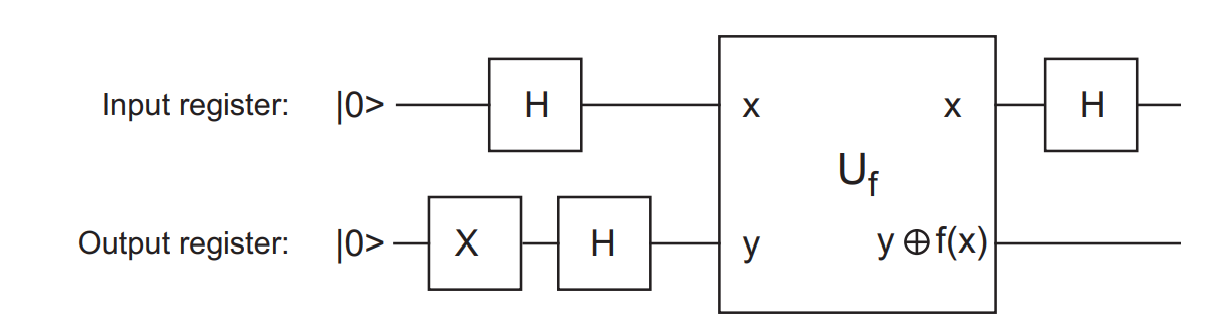
\includegraphics[scale=0.25]{phase1}
\end{figure}
\begin{enumerate}[(a)]
	\item What is the state of the system just before the operator $\U_f$ ?
	
	\item Determine, using what you know about phase kickback, the state of the system just after
	the application of $\U_f$ (and before the final Hadamard) given that you don't know which
	of the four 1-bit to 1-bit functions has been applied.
	\item The four 1-bit to 1-bit functions are defined by the following table.
	
	\begin{center}
	\begin{tabular}{|c|c|c|c|c|}
		\hline
		$x$ & $f_0(x)$ & $f_1(x)$ & $f_b(x)$ & $f_i(x)$ \\
		\hline
		0 & 0 & 1 & 0 & 1\\
		\hline
		1 & 0 & 1 & 1 & 0\\
		\hline
	\end{tabular}
	\end{center}
	What is the state of the system after the application of $\U_f$ (and before the final
	Hadamard) for each of the four functions? What's the difference between constant
	and balanced functions?
	
	\item  What is the state of the system after the final Hadamard gate for each of the four possible
	1-bit to 1-bit functions $\U_f$ ? How can you distinguish constant and balanced functions?
\end{enumerate}


\newpage

\noindent \textit{Solution:}

\begin{enumerate}[(a)]
	\item Just before $\U_f$, the state of the system is given by
	\begin{align}
	\had \ket{ 0} \otimes \had \X \ket{0} = \ket{+-}
	\end{align}
	since $\X$ flips $\ket{0}$ to $\ket{1}$ and $\had\ket{1} = \ket{-}$. 
	
	
	\item We did this in (physical) class. The formula for the output immediately after the application of $\U_f$, provided in the input in the problem is  
	\begin{align}
	\boxed{\ket{\psi} = \f{1}{\sqrt{2}}  \sum_{0 \leq x < 2} (-1)^{f(x)}\ket{x} \otimes \ket{-}   }
	\end{align}
	
	
	\item We do this one by one:
	\begin{align}
	&f = f_{0}: \ket{ \psi } = \f{1}{\sqrt{2}} (\ket{0} + \ket{1})  \ket{-} = \ket{+-}\nn\\
	&f = f_{1}: \ket{ \psi } = \f{1}{\sqrt{2}} (-\ket{0} - \ket{1})  \ket{-} = -\ket{+-}\nn\\
	&f = f_{b}: \ket{ \psi } = \f{1}{\sqrt{2}} (\ket{0} - \ket{1})  \ket{-} = \ket{--}\nn\\
	&f = f_{i}: \ket{ \psi } = \f{1}{\sqrt{2}} (-\ket{0} + \ket{1})  \ket{-} = -\ket{--}
	\end{align}
	Constant functions return Qbits with different handedness, while balanced functions return Qbits with the same handedness. More importantly, constant and balanced functions produce different handedness for Qbit 1. With the Hadamard, we will be able to distinguish these handedness and hence the balanced/constant nature of $f$.
	
	
	
	
	\item If the output immediately after $\U_f$ is $\ket{+-}$ then the final output is $\had_1\ket{+-} = \ket{01}$. If the output immediately after $\U_f$ is $\ket{--}$ then the final output is $\had_1\ket{--} = \ket{11}$. By measuring Qbit 1, we can distinguish constant and balanced functions. If Qbit 1 is in state 0 then $f$ is constant, else $f$ is balanced. 
\end{enumerate}


\qed



\newpage



\noindent \textbf{2.} Consider the output of the Deutsch-Josza problem where the oracle encodes a function $f : \{0, 1\}^n \to \{0, 1\}$ which is known to be either balanced or constant. As shown in the Screencast, after the final set of Hadamards, the state of the input register
is

\begin{align}
\ket{\psi_i} &= \f{1}{2^n}\sum_{0 \leq x < 2^n} (-1)^{f(x)} \sum_{0\leq y < 2^n} (-1)^{x\cdot y} \ket{y}_n \nn\\&= \f{1}{2^n} \sum_{0\leq y < 2^n} \sum_{0\leq x < 2^n}(-1)^{f(x)}(-1)^{x\cdot y}\ket{y}_n.
\end{align}
\begin{enumerate}[(a)]
	\item Show, following the argument made in the Screencast, that the state of the input register $\ket{\psi_i}$ for constant functions leads to a 100\% probability of finding the state in the state $\ket{0}_n$.
	
	\item Show, following the argument made in the Screencast, that the state of the input register $\ket{\psi_i}$ for balanced functions leads to a 0\% probability of finding the state in the state $\ket{0}_n$.
	
	\item Argue, extending the argument made in the Screencast, that the state of the input
	register $\ket{\psi_i}$ for constant functions leads to a 0\% probability of finding the state in some state $\ket{y}_n$ for $y \neq 0$.
	
	\item Argue, extending the argument made in the Screencast, that the state of the input
	register $\ket{\psi_i}$ for balanced functions leads to a nonzero probability of finding the state in the state $\ket{y}_n$ for $y \neq 0$.
\end{enumerate}

\noindent \textit{Solution:}

\begin{enumerate}[(a)]
	\item Suppose $f$ is constant. Then the terms  $(-1)^{f(x)}$ in the sum over $x$ are either all zeros or all ones. This mean we can rewrite the state of the input register as  
	\begin{align}
	\ket{\psi_i} = \pm \f{1}{2^n} \sum_{0\leq y < 2^n} \sum_{0\leq x < 2^n}(-1)^{x\cdot y}\ket{y}_n.
	\end{align}
	Next, we look at the $\ket{0}_n$ term in the sum. Its amplitude is \
	\begin{align}
	\f{\pm 1}{2^n}\sum_{0 \leq x < 2^n} (-1)^{x\cdot 0} = \f{\pm 1}{2^n}\sum_{0 \leq x < 2^n} 1 = \f{\pm 1}{2^n} 2^n = \pm 1.
	\end{align}
	And so there is a $100\%$ probability of finding the state in $\ket{0}_n$. Of course, this leaves zero probability to finding $\ket{\psi_i}$ in any other state. 
	
	

	\item  Suppose $f$ is balanced. Then the terms  $(-1)^{f(x)}$ in the sum over $x$ are either zeros exactly half the time. Consider the summands with $\ket{00}$. This term looks like
	\begin{align}
	\f{1}{2}\sum_{0 \leq x < 2^n} (-1)^{f(x)}(-1)^{x\cdot 0} \ket{0}_n = \f{1}{2}\sum_{0 \leq x < 2^n} (-1)^{f(x)} \ket{0}_n
	\end{align}
	Since $(-1)^{f(x)}$ is $1$ exactly half the time and $-1$ exactly half the time, the amplitude of the state $\ket{0}_n$ is zero. So, the probability that $\ket{\psi_i}$ is in $\ket{0}_n$ is zero.
	
	
	\item Clearly, when the probability that $\ket{\psi_i}$ is in state $\ket{0}_n$ is unity, the probability that $\ket{\psi_i}$ is in any other state is necessarily zero.
	
	
	
	\item Similarly, when the probability that $\ket{\psi_i}$ is in state $\ket{0}_n$ is zero, the probability that $\ket{\psi_i}$ is in any other state is not necessarily zero.
	
\end{enumerate}




\qed


\newpage


\noindent \textbf{3. A quantum decoder.}  Note: This problem is based on an idea from a lecture by John Watrous, who was at the University of Calgary when he wrote it, but is now at the University of Waterloo and is a member of the Institute for Quantum Computing.


In electronics a decoder is a device that sets an output to one for a specific pair of inputs. In the language of quantum computation, an output of a decoder is an oracle that encodes a function of the form $f : \{0, 1\}^2 \to \{0, 1\}$. 

There are four possible decoders, tabulated below.
\begin{center}
	\begin{tabular}{|c|c|c|c|c|}
		\hline
		$x$ & $f_{00}(x)$ & $f_{01}(x)$ & $f_{10}(x)$ & $f_{11}(x)$  \\
		\hline
		00 & 1 & 0 & 0 & 0\\
		\hline
		01 & 0 & 1 & 0 & 0 \\
		\hline 
		10 & 0& 0 & 1 & 0 \\
		\hline 
		11 & 0 & 0 & 0 & 1\\
		\hline
	\end{tabular}
\end{center}

If you didn't know which decoder you had, you would need to query the decoder three times to be sure of what one you had. With phase kickback you can do it in one query.

Consider a device $\U_f$ that encodes one of the four decoders, using the phase kickback approach as shown in the quantum circuit diagram below.

\begin{figure}[!htb]
	\centering
	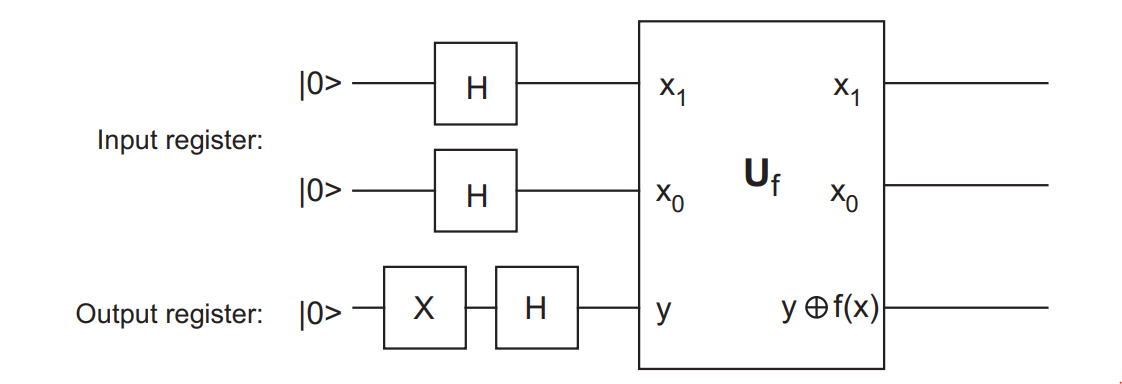
\includegraphics[scale=0.4]{phase2}
\end{figure}

\begin{enumerate}[(a)]
	\item What is the state of the system just before the operator $\U_f$ ?
	\item Determine, using what you know about phase kickback, the state of the system just after
	the application of $\U_f$ given that you don't know which of the decoder circuits has been
	implemented.
	\item Explain why the output for each of the four decoders is an equal superposition of the
	four states ($\ket{00},\ket{01}, \ket{10}, \ket{11}$) with the phase of the ``marked'' state being -1, while all the rest have a phase +1.
	\item These states are all orthogonal entangled states (but not the Bell states). Since they are
	orthogonal, if you (or John Watrous) are clever you can create a quantum circuit that
	disentangle them and put them in basis states of the computational basis. Show that
	for the function $f_{00}$ that circuit below leads to the state $ \ket{\psi(f_{00})} = \ket{00}\ket{-}$.
	\begin{figure}[!htb]
		\centering
		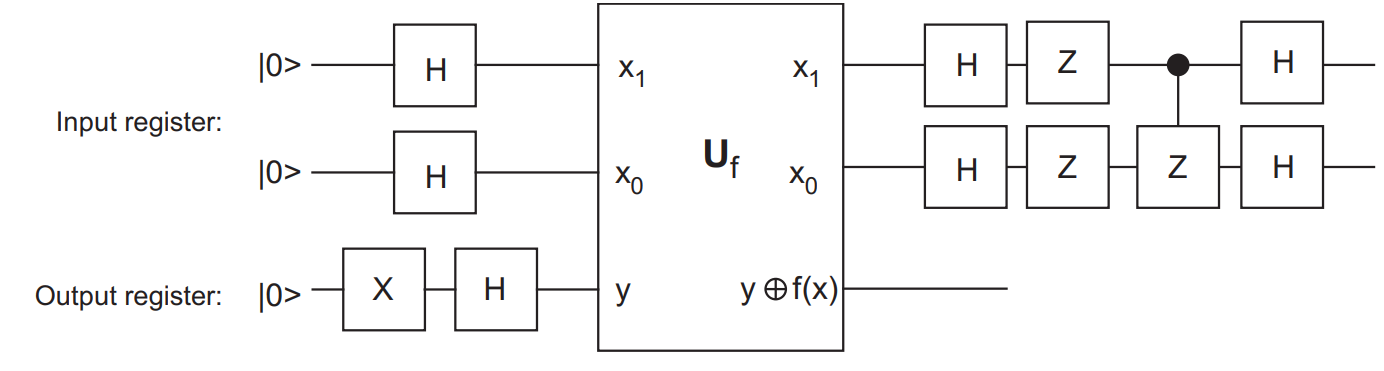
\includegraphics[scale=0.3]{phase3}
	\end{figure}

	\item  (Optional, continuation). Show that the same circuit serves to put the state into the
	appropriate state $\ket{\psi(f_{ij})} = \ket{ij}\ket{-}$.
\end{enumerate}



\noindent \textit{Solution:}


\begin{enumerate}[(a)]
	\item The state of the system just before entering $\U_f$ is 
	\begin{align}
	 \had \otimes \had \otimes \had \X \ket{000} = \had \ket{0} \otimes \had \ket{0} \otimes \had\ket{1} = \ket{++-}.
	\end{align}
	
	
	\item The function $\U_f$ is defined by
	\begin{align}
	\U_f \ket{ x_1 x_0 y} = \ket{ x_1 x_0} \ket{ y \oplus f(x_1x_0)}.
	\end{align}
	
	Given the input $\had^{\otimes n} \ket{0}_n \otimes (\had \X)\ket{0}$ the function $\U_f$ defined above, the output is
	\begin{align}
	\U_f \lc \had^{\otimes n} \ket{0}_n \otimes (\had \X)\ket{0} \rc = \f{1}{\sqrt{2^n}}\sum_{0 \leq x < 2^n}(-1)^{f(x)} \ket{x}_n \otimes \ket{-}.
	\end{align}
	In class we did an example at $n=1$, but it is not hard to see how the example generalizes. The key is the identity: $\ket{ 0\oplus a } = - \ket{1 \oplus a} = (-1)^{f(a)}(\ket{0} - \ket{1}) $. The factor $\lp \ket{ 0} - \ket{1}\rp$ ultimately factors out as a $\ket{-}$ in the formula. \\
	
	Okay, with this, setting $n=2$ (2 input Qbits) we see what the output immediately after $\U_f$ is:
	\begin{align}
	\boxed{\f{1}{\sqrt{2^2}}\sum_{0 \leq x < 2^2}(-1)^{f(x)} \ket{x}_2 \otimes \ket{-}}
	\end{align}
	
	
	\item We can do this in general for any $n$, not just for the $n=2$ case. Say the marked state is $x = \al$, then it follows that $f_\al(x) = 1$ if and only if $x = \al$, and (of course) for $2^n-1$ other times $f_\al(x) = 0$. Look at the output immediately after $\U_f$ again:
	\begin{align}
	\f{1}{\sqrt{2^n}}\sum_{0 \leq x < 2^n}(-1)^{f(x)} \ket{x}_n \otimes \ket{-}.
	\end{align}
	We can write this sum as
	\begin{align}
	 &\f{1}{\sqrt{2^n}}(-1)^{f_\al(\al)}\ket{ \al}\otimes \ket{-} + \f{1}{\sqrt{2^n}}\sum_{\substack{{0 \leq x < 2^n}\\ {x\neq \al}}} (-1)^{f_\al(x)} \ket{x}_n \otimes \ket{-}\nn\\
	 =& \f{1}{\sqrt{2^n}} (-1)\ket{\al}\otimes \ket{-} + \f{1}{\sqrt{2^n}}\sum_{\substack{{0 \leq x < 2^n}\\ {x\neq \al}}} (1)\cdot \ket{x}_n   \otimes \ket{-}.
	\end{align}
	So, we see that not only this is an equal superposition of all computational basis states, it is also one where the marked state $\ket{\al}$ carries a phase of $(-1)$, while the other states $+1$. And to get an exact answer for item (c), we can just let $n=2$. 
	
	
	
	\item Assume $f = f_{00}$. Then the output immediately after $\U_f$ is given by
	\begin{align}
	\f{1}{\sqrt{2^2}}\sum_{0 \leq x < 2^2}(-1)^{f_{00}(x_1x_0)}\ket{x_1x_0} \otimes \ket{ - }.
	\end{align}   
	Since all operators act on the two input Qbits, we can just ignore that output Qbit for now. The evaluation is straightforward (provided no malicious typos appear)
	\begin{align}
	&\,\had^{\otimes 2}\mathbf{C}_{21}^\Z\Z^{\otimes 2}\had^{\otimes 2}\f{1}{\sqrt{2^2}}\sum_{0 \leq x < 2^2}(-1)^{f_{00}(x_1x_0)}\ket{x_1x_0}\nn\\
	=\,& \f{1}{2}\had^{\otimes 2}\mathbf{C}_{21}^\Z \Z^{\otimes 2}\had^{\otimes 2}\lb -\ket{00} + \ket{01} +  \ket{10} + \ket{11} \rb\nn\\
	=\,& \f{1}{2}\had^{\otimes 2}\mathbf{C}_{21}^\Z \Z^{\otimes 2} \lb -\ket{++} + \ket{+-} + \ket{-+} + \ket{--}  \rb\nn\\
	=\,& \f{1}{2}\had^{\otimes 2}\mathbf{C}_{21}^\Z \lb -\ket{--} + \ket{-+} + \ket{+-} + \ket{++} \rb\nn\\
	=\,& \f{1}{2}\had^{\otimes 2}\mathbf{C}_{21}^\Z \lb \sqrt{2}\ket{1}\ket{-} + \sqrt{2}\ket{0} \ket{+} \rb\nn\\
	=\,& \f{1}{\sqrt{2}}\had^{\otimes 2}\mathbf{C}_{21}^\Z\lb \ket{1}\ket{-} + \ket{0} \ket{+} \rb\nn\\
	=\,& \f{1}{\sqrt{2}}\had^{\otimes 2} \lb \ket{1}\ket{+} + \ket{0}\ket{+} \rb\nn\\
	=\,& \had^{\otimes 2}\ket{++}\nn\\
	=\,& \ket{00}.
	\end{align}
	And so the final state of the system is $\ket{00}\ket{ - }$. 
	
	
	
	
	\item How do we do this in general? Since there are only 3 more cases, it's worth doing this by exhaustion. We already know what happens when $i=j=0$. Now consider $i=0, j=1$. In this case, $\ket{01}$ will carry a $-1$ phase, which turns the seventh line to $\sim \had^{\otimes 2} \lb -\ket{1}\ket{-} + \ket{0}\ket{-} \rb \sim \had^{\otimes 2}\ket{+-} = \ket{01}$. When $i=j=1$, the state $\ket{11}$ carries the $-1$ phase. This turns the sixth line $\mathcal{O}\lb \ket{0}\ket{-} - \ket{1}\ket{+} \rb$ where $\mathcal{O}$ is a combination of operators and scalars. Applying $\mathbf{C}_{21}^{\Z}$, followed by $\had^{\otimes}$, gives $\had^{\otimes 2}\ket{--} = \ket{11}$. By elimination, we know when $i=1,j=0$, the output is going to be $\ket{10}$. But we can also check (why not?). When $i=1,j=0$, the term $\ket{10}$ carries a $-1$ phase. This result in the sixth line being $\sim \mathcal{O}[\ket{0}\ket{+} + \ket{1}\ket{-}]$. Applying $\mathbf{C}_{21}^{\Z}$ followed by $\had^{\otimes 2}$ gives $\had^{\otimes 2} \lp \ket{0}\ket{+} - \ket{1}\ket{+} \rp \sim \had^{\otimes 2}\ket{-+} = \ket{01}$. \\
	
	To summarize:
	\begin{center}
	\begin{tabular}{|c|c|c|}
		\hline
			& $j=0$ & $j=1$ \\
		\hline
		$i=0$ & $\to\ket{00}$ &  $\to\ket{01}$\\
		\hline
		$i=1$ & $\to\ket{10}$ & $\to\ket{11}$ \\
		\hline
	\end{tabular}
	\end{center}

	We conclude that $\ket{\psi (f_{ij})} = \ket{ij}\ket{-}$.
	
\end{enumerate}







\qed



\newpage

\noindent \textbf{4. Bernstein-Vazirani without Phase Kickback.}  The idea of this problem is to look again
at the Bernstein-Vazirani problem without using phase kickback as an introduction to the
techniques used for Simon’s problem. 

Recall that in the Bernstein-Vazirani problem you are given a function $f : \{0, 1\}^n \to \{0, 1\}$ that encodes a hidden bit-string a such that $f(x) = a \cdot x$ (mod 2) for any input string $x$.

Consider the circuit below that implements a 2-Qbit version of the Bernstein-Vazirani problem
with the string $a = 10$.

\begin{figure}[!htb]
	\centering
	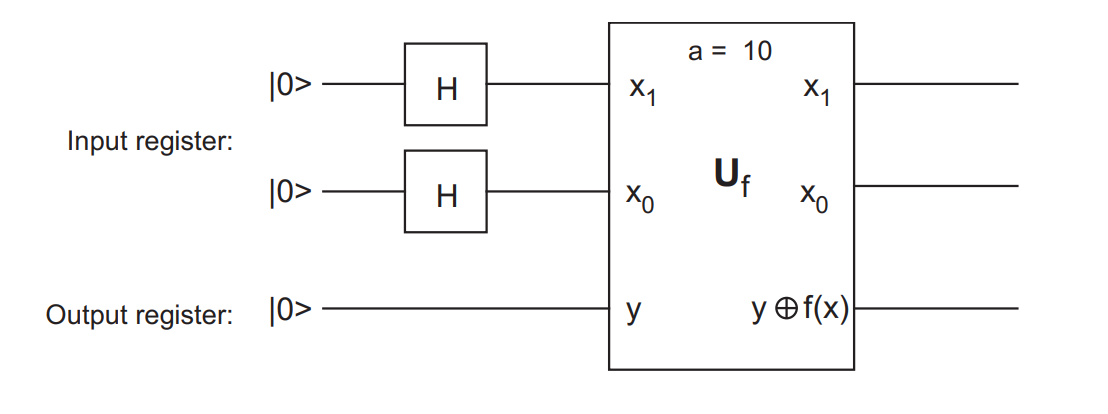
\includegraphics[scale=0.25]{phase4}
\end{figure}


\begin{enumerate}[(a)]
	\item What is the state of the system after the application of $\U_f$?
	\item Are the input and output registers entangled? How do you know?

	\item Imagine that you measured the output register and found that the output register was
	in the state $\ket{1}$. What is the state of the system after that (partial) measurement?

	\item Look at the solution you got, and note that the states $\ket{x_i}$ of the input register correspond to states with $a \cdot x_i = 1$.
	\item  Imagine that you measured the output register and found that the output register was in the state $\ket{0}$. What is the state of the system after that (partial) measurement?
	\item  Look at the solution you got, and note that the states $\ket{x_j}$ of the input register correspond to states with $a \cdot x_j = 0$. Of course if you measured the output you would only find one
	of the states.

	\item Now, after measuring $y$ and $x$ this way a couple of times you would have a set of equations
	$a \cdot x = 0 \text{ or } a \cdot x = 1$ for different x values. Convince yourself that you could use these values to figure out $a$. (Unless you are unlucky and get $x = 0$, which tells you nothing,
	because $a \cdot 0 = 0$ for all $a$.)

\end{enumerate}

Note: This approach is no more efficient than a classical algorithm would be if you randomly
chose input values. The importance of this approach – using multiple queries and then using
the resulting classical answers to determine the behavior of the oracle – was recognized by
Dan Simon for a function $f : \{0, 1\}^n \to \{0, 1\}^n$.\\







\newpage


\noindent \textit{Solution:}

\begin{enumerate}[(a)]
	\item The state of the system immediately after the application of $\U_f$ is 
	\begin{align}
	\U_f (\had_2\had_1 \ket{000}) 
	&= \U_f \ket{++0} \nn\\
	&= \f{1}{2}\U_f \lb \ket{00} + \ket{01} + \ket{10}+ \ket{11} \rb \otimes \ket{0}\nn\\
	&= \f{1}{2}\lb \ket{00f(00)} + \ket{01f(01)} + \ket{10f(10)}+ \ket{11f(11)}  \rb\nn\\
	&= \f{1}{2} \lb \ket{000} + \ket{010} + \ket{101} + \ket{111} \rb\nn\\
	&= \f{1}{\sqrt{2}} \ket{0 + 0} + \f{1}{\sqrt{2}} \ket{1 + 1} .
	\end{align}
	where $f(x) \equiv_2 a\cdot x$.
	
	\item  The state of the system immediately after the application of $\U_f$ is entangled. In particular, the Qbit in the output register is entangled with the top input Qbit. Whenever the Qbit in the output register is in state $i$, the top Qbit in the input register is also in state $i$.
	
	\item Suppose the state of the output register is $\ket{1}$. Then the state of the input register is $\ket{1+}$. The state of the system as a result of the measurement is $\ket{1+1}$. 
	
	\item Suppose the output Qbit is in state $\ket{1}$. The input register is in the states $\ket{10}$ and $\ket{11}$. Clearly, $a\cdot x_i = 10 \cdot 11 = 10 \cdot 10 = 1$.  
	
	\item Suppose the output Qbit is in state $\ket{0}$. The state of the system after that measurement collapses to $\ket{0 + 0}$. 
	
	
	\item Whenever the output Qbit is in state $\ket{0}$, the input register is in states $\ket{01}$ and $\ket{00}$. So, $a\cdot x_j = 10 \cdot 01 = 10 \cdot 00 = 0$.  
	
	\item In the context of this problem, $a \cdot x = 0$ whenever $x = 0$ or $x = 1$, and $a \cdot x=  1$ whenever $x = 2$ or $x=3$. When $x=0$, we don't learn anything (but this is fine because when size of the vector space grows exponentially as the problem gets bigger, this possibility is small). When $x=1$, because $a \cdot 1 = 0$ we know that $a = a_1 a_0 = a_1 0$. Next, because $a \cdot 2 = a \cot 3 = 1$, $a_1 = 1$. This gives $a = 10$. 
\end{enumerate}






\qed


\newpage















\section{Problem set 8}


\noindent \textbf{1. A Simon's Algorithm Primer.} You are given a unitary operator $\U_f$ that encodes a function $f: \{0,1\}^n \to \{0,1\}^n$ for a 3-bit input ($n = 3$) which has the characteristics $f(x) = f(x\oplus a)$ for an unknown $a$ -- but it is known that $a\neq 0$. \\

\begin{figure}[!htb]
	\centering
	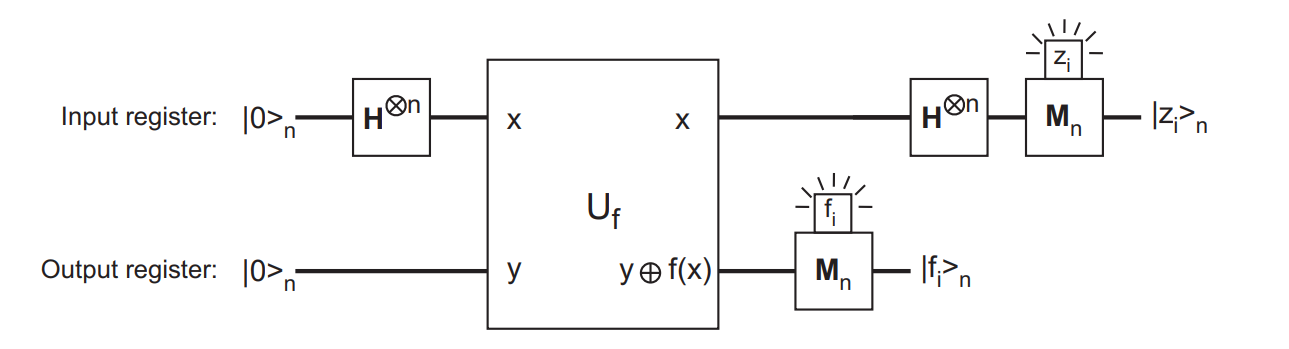
\includegraphics[scale=0.5]{simon1}
\end{figure} 

The outputs of the specific function $f(x)$ for the eight possible inputs are tabulated below.


\begin{center}
	\begin{tabular}{|c|c|c|}
		\hline
		\multicolumn{1}{c}{} & \multicolumn{1}{c}{$x$} & \multicolumn{1}{c}{$f(x)$}\\
		 \hline
		0 & 000 & 110\\
		\hline
		1 & 100 & 000\\
		\hline
		2 & 010 & 001\\
		\hline
		3 & 011 & 101\\
		\hline
		4 & 100 & 000\\
		\hline
		5 & 101 & 110\\
		\hline
		6 & 110 & 101\\
		\hline
		7 & 111 & 001\\
		\hline
	\end{tabular}
\end{center}





\begin{enumerate}[(a)]
	\item Use a classical algorithm (look for collisions) and determine the hidden string $a$.
\end{enumerate}

For the rest of this problem, consider the quantum algorithm for solving Simon's problem shown in the circuit diagram above.


\begin{enumerate}[(a)]\setcounter{enumi}{1}
	\item What is the state of the system $\ket{\psi_1}$ just before the oracle?

	
	\item What is the state of the system $\ket{\psi_2}$ just after the oracle? 
	
	
	\item What is the state of the system $\psi_3$ just after a measurement of the output register gave the value $f_0 = 001$?

	
	
	\item  What is the state of the system $\ket{\psi_4}$ after the final set of Hadamard operations on the
	input register (and, of course, after the measurement of $f_0 = 001$)?
	
	
	\item Show that each component of the input register $\ket{z_i}$ has the property $z_i \cdot a = 0$ (using the value of a you found in part (a)) and that the states $\ket{z_j}$ \textbf{not} included in the superposition
	have the property $z_j \cdot a = 1$. 
	
	
	\item Go back a step and consider a second query of the oracle. Since the input $\ket{\psi_1}$ is the same as the output of the oracle $\ket{\psi_2}$ is also the same. What is the state of the system $\ket{\psi_3}$ just after the measurement  of the output register gave the value $f_1 = 101$? 
	
	
	
	\item What is the state of the system $\ket{\psi_4}$ after the final set of Hadamard operations on the input register (and, of course, after the measurement of $f_1 = 101$)? Compare the input register state with the one in part (e). 
	
	
	
	
	\item Suppose that after your two queries of the oracle, measurements of the input register
	gave $z_0 = 010$ and $z_1 = 111$. Show, that (if is known that $a\neq 000$) these two measurements determine the value of $a$. If it's not known that $a\neq 000$ then $a=0$ is a
	solution as well no matter what the values of $z$ are. 
\end{enumerate}





\noindent \textit{Solution:}

\begin{enumerate}[(a)]
	\item We know that $f$ is a $2$ to $1$ function. So, it suffices to look at two inputs $x_0\neq y_0$ such that $f(x_0) = f(y_0)$.  In this case, we necessarily have $x_0 = y_0 \oplus a$. Since we're working over the finite field $\mathbb{F}^{2n}$, we know that
	\begin{align}
	x_0 &= y_0 \oplus a \nn\\
	\iff x_0\oplus y_0 &= y_0 \oplus y_0 \oplus a, \quad \text{addition is commutative}\nn\\
	\iff x_0 \oplus y_0 &= a.
	\end{align}
	From the table, we know that $001$ and $100$ give the same output $000$. And so $a = 001 \oplus 100 = 101$. So, $\boxed{a= 101}$. As a sanity check, $000\oplus 101 = 010 \oplus 111 \oplus 011 \oplus 110 = 101$ as well. 
	
	
	
	\item Just before the oracle, the state of the system is 
	\begin{align}
	\ket{\psi_1} &= (\had^{\otimes n}\otimes \Id^{\otimes n}) \ket{0}_n \ket{0}_n\nn\\
	&= \f{1}{\sqrt{2^n}} \sum_{0 \leq x < 2^n} \ket{x}_n \ket{0}_n\nn\\
	&= \f{1}{\sqrt{2^3}} \sum_{0 \leq x < 2^3} \ket{x}_3 \ket{0}_3, \quad n=3.
	\end{align}
	
	
	
	
	
	
	\item The state of the system just after the oracle is 
	\begin{align}
	\ket{\psi_2} &= \U_f \ket{\psi_1}\nn\\
	&= \U_f \f{1}{\sqrt{2^3}} \sum_{0 \leq x < 2^3} \ket{x}_3 \ket{0}_n\nn\\
	&= \f{1}{\sqrt{2^3}} \sum_{0 \leq x < 2^3} \ket{x}_3 \ket{f(x)}_3.
	\end{align}
	
	
	
	\item If $x_0 = 001$, then after the measurement the state of the system must carry $\ket{001}$ in the output register. Since $f$ is 2-to-1, there are two states with the output register in $\ket{001}$. So, 
	\begin{align}
	\ket{\psi_3} = \f{1}{\sqrt{2}} \lb \ket{010} + \ket{111} \rb \ket{001}.
	\end{align}
	
	
	
	\item To find the state after Hadamard-ing the input register, we just go through the straightforward computation:
	\begin{align}
	\ket{\psi_4} &= \had^{\otimes 3} \otimes \Id^{\otimes 3} \f{1}{\sqrt{2}}\lb \ket{010} + \ket{111} \rb \ket{001}\nn\\
	&= \f{1}{\sqrt{2}}\lb \ket{+-+} + \ket{---} \rb \ket{001}\nn\\
	&= \f{1}{\sqrt{2}} \f{1}{\sqrt{2^3}}\lb \ket{000} - \ket{010} + \ket{101} - \ket{111}  \rb\ket{001}.
	\end{align} 
	
	
	
	\item We can see easily that each component-state $z_i$ of the input register is such that $z_i \cdot a = 0$:
	\begin{align}
	&000 \cdot 101 = 0 \oplus 0 \oplus 0 = 0\nn\\
	&010 \cdot 101 = 0 \oplus 0 \oplus 0 = 0\nn\\
	&101 \cdot 101 = 0 \oplus 0 \oplus 0 = 0\nn\\
	&111 \cdot 101 = 0 \oplus 0 \oplus 0 = 0.
	\end{align} 
	We can also see states that are not those above have the property that $z_j \cdot a = 1$:
	\begin{align}
	&001 \cdot 101 = 0 \oplus 0 \oplus 1 = 1\nn\\
	&011 \cdot 101 = 0 \oplus 0 \oplus 1 = 1\nn\\
	&100 \cdot 101 = 1 \oplus 0 \oplus 0 = 1\nn\\
	&110 \cdot 101 = 1 \oplus 0 \oplus 0 = 1.
	\end{align} 
	
	
	
	
	\item  If $f_1 = 101$, then $\ket{\psi_3} \sim \lb \ket{011} + \ket{110} \rb \ket{101}$. Normalizing this gives
	\begin{align}
	\ket{\psi_3} = \f{1}{\sqrt{2}}\lb \ket{011} + \ket{110} \rb\ket{101}.
	\end{align}
	
	
	
	
	
	\item Hadamard-ing to the input register we get $\ket{\psi_4} \sim \lb \ket{+--} + \ket{--+} \rb \ket{101} \sim \lb \ket{000} - \ket{010} - \ket{101} + \ket{111} \rb \ket{101}$. We see that the components of the input register in this case is the same as before. Of course, after normalization,
	\begin{align}
	\ket{\psi_4} = \f{1}{\sqrt{2}}\f{1}{\sqrt{2^3}} \lb \ket{000} - \ket{010} - \ket{101} + \ket{111} \rb \ket{101}.
	\end{align}
	
	

	\item Let $a = a_2a_1a_0 \neq 000$. If measurements of the input register gives $z_0 = 010$ and $z_1 = 111$, then we know that $0= 010 \cdot a_2 a_1 a_0 = 111 \cdot a_2 a_1 a_0 = 0$. The first equality tells us that $a_1 = 0$. The last equality tells us that $a_2 \oplus 0 \oplus a_0 = 0$, which means $a_2 = a_1 = 1$ (since they can't both be 0). So $a = 101$, as expected. 
	
	
	
	
	
	
\end{enumerate}\qed






\newpage









\noindent \textbf{2. A Simon's Algorithm Primer'.} You are given a unitary operator $\U_f$ that encodes the function $f : \{0,1\}^n \to \{0,1\}^n$ which has the characteristics $f(x) = f(x\oplus a)$ but this time for $a=0$. The fact that $a = 0$ means that every output value of $f(x)$ is distinct -- the function is one-to-one.	\\

Show that employing the circuit diagram from the prior problem will lead to set of all $2^n$ possible states of the input register, each with an equal probability $P_i = 1/2^n$ of being measured in the final step of the algorithm.\\

Notice that in this case (if you didn’t know that $a = 0$ and weren't assured that $a \neq 0$) if
you just ran the algorithm you could also generate a set of equations satisfying $a \cdot z_i = 0$ for
$0 \leq i \leq n_1$. If you did the same classical post-processing (solving the equations for $a$ you
would get some nonzero value. Of course all states satisfy $a \cdot z_i = 0$ if $a = 0$. You'd then have
to check two inputs $x$ and $x \oplus a$ to the oracle - maybe $\ket{000}$ and $\ket{a}$ - and see if they have the
same output value. If not then you know $a = 0$.
\\


\noindent \textit{Solution:} When $a = 0 \implies f$ is 1-to-1 (and onto), we have, by looking at $\ket{\psi_2}$ in the previous problem, that each $\ket{x}$ goes with a distinct $\ket{f(x)}$. This means $\ket{\psi_3}$ is a tensor product of two n-Qbit computational basis states: the first is that of the input register, the second is that of the output register.  Because the input register is now in a basis state, Hadamard-ing it gives an equal superposition of all $2^n$ computational basis states without destructive interference (unlike in the previous problem where this happens). This means each state of the input register has an amplitude $1/\sqrt{2^n}$, which corresponds to a probability $P_i = 1/2^n$ of being measured. \qed








\end{document}